\documentclass[11pt]{amsart}

\usepackage{amsmath,amssymb,amsthm,mathtools}
\usepackage{booktabs,tabularx,array}
\usepackage{graphicx}
\usepackage{tikz,tikz-cd}
\usetikzlibrary{arrows.meta,calc,decorations.markings,patterns,positioning,shapes.geometric}
\usepackage{adjustbox}
\usepackage[margin=1.15in]{geometry}
\usepackage[colorlinks=true,linkcolor=blue,citecolor=blue,urlcolor=blue]{hyperref}
\usepackage{microtype}
\emergencystretch=1.5em

\newtheorem{theorem}{Theorem}[section]
\newtheorem{maintheorem}{Theorem}
\renewcommand{\themaintheorem}{\Alph{maintheorem}}
\newtheorem{proposition}[theorem]{Proposition}
\newtheorem{corollary}[theorem]{Corollary}
\newtheorem{lemma}[theorem]{Lemma}
\theoremstyle{definition}
\newtheorem{definition}[theorem]{Definition}
\newtheorem{example}[theorem]{Example}
\newtheorem{construction}[theorem]{Construction}
\newtheorem{problem}[theorem]{Problem}
\newtheorem*{mainproblem}{Problem C}
\theoremstyle{remark}
\newtheorem{remark}[theorem]{Remark}
\newtheorem*{importedthm}{Theorem}

\newcommand{\PP}{\mathbb P}
\newcommand{\CC}{\mathbb C}
\newcommand{\ZZ}{\mathbb Z}
\newcommand{\QQ}{\mathbb Q}
\newcommand{\RR}{\mathbb R}
\newcommand{\NN}{\mathbb N}
\newcommand{\Acal}{\mathcal A}
\newcommand{\Lcal}{\mathcal L}
\newcommand{\Mcal}{\mathcal M}
\newcommand{\Ocal}{\mathcal O}
\newcommand{\Tcal}{\mathcal T}
\newcommand{\Wcal}{\mathcal W}
\newcommand{\Xfrak}{\mathfrak X}
\newcommand{\Dscr}{\mathfrak D}
\newcommand{\Spec}{\operatorname{Spec}}
\newcommand{\Spf}{\operatorname{Spf}}
\newcommand{\Aut}{\operatorname{Aut}}
\newcommand{\Hol}{\operatorname{Hol}}
\newcommand{\Sym}{\operatorname{Sym}}
\newcommand{\Corr}{\operatorname{Corr}}
\newcommand{\BL}{\operatorname{BL}}
\newcommand{\Jac}{\operatorname{Jac}}
\newcommand{\GKT}{\mathrm{GKT}}

\hyphenation{scat-ter-ing tropi-cal singu-lar-ity de-scen-dent
pro-al-ge-bra-ic Kum-mer log-a-rith-mic}

\title[Annular scattering in open FJRW theory]
{Annular scattering in quartic open FJRW theory}
\author{Bernd Johannes Wuebben}
\subjclass[2020]{14T90 (primary); 14B07, 14D06, 14J33, 14N35, 32S25, 32S30 (secondary)}
\keywords{Scattering diagrams, integral-affine manifolds, logarithmic mirror
symmetry, root stacks, Jacobi structures, open FJRW theory}
\date{September 29, 2026}
\hypersetup{
  pdftitle={Annular scattering in quartic open FJRW theory},
  pdfauthor={Bernd Johannes Wuebben},
  pdfsubject={Annular scattering in quartic open FJRW theory},
  pdfkeywords={scattering diagrams, integral-affine manifolds, logarithmic mirror symmetry, open FJRW theory}
}

\begin{document}

\begin{abstract}
Gross--Siebert mirrors come from integral-affine bases with
singularities; we ask whether open Landau--Ginzburg wall-crossing supplies
such a base.  For the open FJRW theory of $x^4+y^4$ of Gross, Kelly and
Tessler (GKT), a double cover of the Carl--Pumperla--Siebert disk
is forced; it carries walls, but not GKT wall-crossing.  Send $x^ay^b$
to $z^{F(a,b)}$, for $F$ linear sending $x^4,y^4$ to the rays of $\{X=0\}$,
$\{Y=0\}$ in the fan lattice of $\PP(1,1,2)$, which is the exponent lattice
of that disk.  The two first-order descendent GKT generators have
fractional exponents, spanning an overlattice of index eight.  The minimal
cover preserving it is an integral-affine annulus with two focus--focus
singularities, two points at which it is a focus--focus singularity pulled
back by $z\mapsto z^2$, and core holonomy of trace $18$.  The slab-function
roots lifting the monodromy have an infinite transport orbit and rescale
$dx\wedge dy$, whose Poisson bracket glues only as a Jacobi bracket.
Placed along gradient images of their exponents for an $x$--$y$ symmetric
quadratic function, the two generators and their Kontsevich--Soibelman
factors give walls consistent to all orders at the two lifts of the central
vertex.

The GKT Lie algebra embeds in this bracket's Hamiltonian derivations, but on
the lowest-order wall involving both generators the coefficient is $-3/4$
where GKT's is $1/4$.  The potentials $W^{\min}$, $W^{\max}$ of GKT's
extremal boundary conditions keep, for each label set, only the
balanced-graph coefficient of least, respectively greatest, $x$-degree.  For
two labels with one descendent each, transport through the walls carries
$W^{\min}$ to $W^{\max}$ up to the flow of one GKT generator, which the
normal form keeping only coefficients of greatest $x$-degree removes; its
geometric realization is open.  GKT's canonical homotopies can be chosen
compatibly as the label set grows.
\end{abstract}

\maketitle

\section{Introduction}\label{sec:introduction}

Throughout, $\Bbbk$ is an algebraically closed field of characteristic
zero.  Formal-algebraic constructions are made over $\Bbbk$; oscillatory
integrals and Saito theory are understood after base change to $\CC$.
The enumerative coefficient rings are defined over $\QQ$ and are implicitly
base-changed to $\Bbbk$ when used in the root-stack construction.

\subsection{From boundary-ray continuation to an affine scattering problem}

The Gross--Siebert programme constructs mirrors by placing wall-crossing
automorphisms on an integral-affine base with singularities and reading off
broken lines and theta functions
\cite{grosshackingkeel2015,grossetal2018canonical,grosssiebert2022}.  What it
requires as input is geometric: a base, its singular locus, a polyhedral
decomposition, and a polarization.  This paper asks whether the wall crossing
of an open Landau--Ginzburg theory supplies that input, and settles the
question for one model.

Gross, Kelly, and Tessler define genus-zero open FJRW invariants for
\[
 (W,G)=\bigl(x^r+y^s,\mu_r\times\mu_s\bigr)
\]
as relative Euler numbers on moduli spaces of $W$-spin disks
\cite{grossetal2022open}.  Their invariants depend on canonical
multisections, and changes of those boundary conditions act through a formal
wall-crossing group closely related to the tropical vertex group.  This
action has the algebra of a scattering diagram but not, by itself, an
integral-affine realization: there is no affine manifold, singular locus, or
polyhedral decomposition on which the walls have been placed.

The companion paper \cite{wuebben2026boundary} isolates the gap precisely.

\begin{importedthm}[Boundary-ray factorization \cite{wuebben2026boundary}]
\label{thm:companion}
Fix a finite set of deformation monomials closed under taking divisors.  After
discarding every other monomial, the change between the two canonical GKT
boundary conditions at the limiting boundary rays factors uniquely into
wall-crossing operations ordered by slope.  The slope of a factor is the ray
spanned by the pair of boundary-marking counts of the corresponding critical
$W$-spin graph.  Each factor is realized by a homotopy of canonical boundary
conditions.  Radial motion in the punctured first quadrant of marking counts
acts trivially, so the product is transport from one limiting ray to the other
and not monodromy around the origin.  After the degree-zero torus action is
included, the two endpoint boundary conditions and their transition are
unique in the finite quotient.  The nonidentity factors admit successive
finite homotopies in increasing-slope order.
\end{importedthm}

This result supplies an ordered family of wall-crossing operations, but it
does not supply the integral-affine surface on which their rays should lie or
any affine monodromy.  The present paper constructs that missing geometry.

We resolve this for the parabolic quartic
\[
 W=x^4+y^4,
\]
the parabolic singularity $X_9$, whose central charge is exactly one.  The
suspension of its marginal pencil is an anticanonical elliptic curve in
$\PP(1,1,2)$, and the toric-boundary degeneration of that pair gives the
disk-shaped dual intersection complex of the Landau--Ginzburg construction of
Carl--Pumperla--Siebert \cite{carletal2024}; we call it the \emph{CPS
complex}.  It is the natural candidate base.  The first result of this paper
is that it cannot carry the descendent lattice, and that three further
standard choices fail with it: a finite
root stack of coefficients, a scalar Hamiltonian algebra, and a theta basis
indexed by one lattice.  Proposition~\ref{thm:intro-obstructions} collects the
five obstructions, each proved in the body.

\subsection{Initial Hamiltonians}

The affine and scattering constructions begin with two elements of the GKT
critical Lie algebra.  Write $M=\ZZ^2$ for the toric character lattice in the
chosen toric chart.  A
critical graph of \cite{grossetal2022open}
is supported on a nonempty set $J$ of boundary markings, each carrying a
descendent order; we call the datum a \emph{singleton} when $|J|=1$, and \emph{primary} when no marking carries a
positive descendent order.  The two first-order singleton generators of
$x^4+y^4$ are, writing $q^\perp=(q_2,-q_1)$, $\partial_v$ for the invariant
logarithmic derivation in direction $v$, and $\kappa=(1,1)$ for the shift
introduced below, in the shifted notation
$X^\kappa_q=z^{q-\kappa}\partial_{q^\perp}$ of
Section~\ref{sec:jacobi-theta},
\[
 \mathsf A=-\tfrac12t_1X^\kappa_{(2,1)},
 \qquad
 \mathsf B=-\tfrac12t_2X^\kappa_{(1,2)},
\]
the coefficient $-\tfrac12$ being the normalization borne by the GKT
invariants themselves.  The integer pairs $(2,1)$ and $(1,2)$ label the
generators and do lie in $M$.  Their wall supports are obtained by the
cofactor map $F$ in \eqref{eq:intro-F}:
\[
 F(2,1)=(1/4,-1/2),\qquad F(1,2)=(-1/4,-1).
\]
These support vectors do not lie in $M$; their integral span with $M$ is the
index-eight overlattice $\widetilde M$.  This is the lattice mismatch that
produces the annular cover of Section~\ref{sec:affine-kummer}.  We call
$\mathsf A$ and $\mathsf B$ the \emph{singleton
Hamiltonians}, and we call their deformation parameters $t_1,t_2$ the
\emph{singleton parameters}; the ideal $I=(t_1,t_2)$ is the \emph{singleton
ideal}.  These two elements are the only enumerative input to
Sections~\ref{sec:affine-kummer}--\ref{sec:compactification}.  We call
$X_{0,0}=x\partial_x-y\partial_y$ the \emph{degree-zero} generator; the word
\emph{marginal} is reserved throughout for the charge-one deformation
direction $x^2y^2$, the modulus of $X_9$.  An element of $\mu_4\times\mu_4$
is \emph{narrow} when its fixed locus in $\CC^2$ is the origin; the nine
narrow elements are $(\zeta^{a+1},\zeta^{b+1})$ with $0\leq a,b\leq2$, matching
the monomial basis $x^ay^b$ of the Jacobian ring $\Jac(x^4+y^4)$.

\subsection{Coefficient system and volume line}

Two consequences of the lattice mismatch determine the coefficient system.
Let a \emph{finite transport tree} be a finite rooted tree whose vertices are
chambers of the annular wall decomposition and whose oriented edges are
reduced paths between adjacent chambers.  For such a tree $T$ and an integer
$N$, adjoining the finitely many roots required to lift every slab and wall
map along $T$, and then reducing modulo $I^N$, gives a finite root stack
$\mathcal R_{T,N}$.  Inclusion of trees, refinement of paths, and reduction of
$N$ give transition maps.  We use the inverse system
\begin{equation}
 \{\mathcal R_{T,N}\}_{(T,N)}
 \label{eq:intro-root-system}
\end{equation}
over this cofiltered category; no geometric inverse limit is asserted.  It is
formally analogous to the finite stages of an infinite root stack
\cite{talpovistoli2018}, but the indexing category here records path transport
rather than divisibility alone.

The second uses a twisted volume form.  In a developed torus chart put
\[
 \kappa=(1,1),\qquad
 \Omega_\kappa=z^\kappa\,d\log z_1\wedge d\log z_2.
\]
$\kappa$ denotes the shift in the chosen developed chart and is transported
with that chart; it is not a global flat section of the character local
system.  A lifted slab transition preserves
$d\log z_1\wedge d\log z_2$ but rescales
$\Omega_\kappa$ by a root-valued unit, so the local Hamiltonian brackets glue
on a line bundle rather than on the structure sheaf.  The resulting object is
the Jacobi--Kirillov bracket on the \emph{volume line} $\Lcal_\kappa$;
equivalently, the complement of the zero section in $\Lcal_\kappa^\vee$ carries
a homogeneous Poisson structure, the Poissonization of the Jacobi bracket
\cite{vitaglianowade2016}.  Saito's primitive form is a different object and
enters only in Section~\ref{sec:primary-frobenius}.

\subsection{Annular monodromy and its consequences}

Two mechanisms produce the departures from the standard finite-type
situation.  The first descendent exponents force an overlattice
$\widetilde M\supset M$ of index eight; only one of the three affine
monodromies of the CPS complex preserves it; the double cover branched at the
two offending singular points is an annulus; and the holonomy $K$ of that annulus about
its core has trace $18$, hence is hyperbolic.  Repeated slab shear makes the
transported root orbit infinite and forces the inverse system
\eqref{eq:intro-root-system}.
Hyperbolicity makes every nonzero exponent orbit infinite and forces the theta
functions to form a local system rather than a basis indexed by one lattice.

\subsection{Basic notation}

We use the standard scattering-diagram terminology of
\cite{grosssiebert2022}.  In particular, slabs carry the gluing functions on
codimension-one cells, whereas walls are outgoing.  The cofactor map below
determines the supports of the two initial Hamiltonians.

Let $M\simeq\ZZ^2$ be the character lattice of the quartic toric model,
$\varphi$ its polarization, and, in the cofactor chart of
Section~\ref{sec:affine-kummer}, put
\begin{equation}\label{eq:intro-F}
 F=\frac14\begin{pmatrix}1&-1\\0&-2\end{pmatrix},
 \qquad \widetilde M=F(\ZZ^2),
 \qquad D=\widetilde M/M\simeq\ZZ/2\oplus\ZZ/4.
\end{equation}
Let $\overline\Acal$ be the completed parity cover,
$\Acal=\operatorname{Int}(\overline\Acal)$, and let
$\Acal^\circ$ be the complement of its four affine singularities.  We write
$t_{a,b}$, $0\leq a,b\leq2$, for the primary deformation parameters dual to
the monomial basis $x^ay^b$ of $\Jac(x^4+y^4)$, which index the nine narrow
sectors, and reserve $t_1,t_2$ for the singleton parameters of \S1.2.  The linear holonomy of $\Acal$ about its
core, in the basis of $\widetilde M$ fixed by $F$ and with the orientation of
Appendix~\ref{app:calculations}, is
\begin{equation}\label{eq:intro-K}
 K=\begin{pmatrix}-1&2\\-10&19\end{pmatrix},
 \qquad \operatorname{tr}K=18.
\end{equation}

\subsection{Obstructions to the disk-shaped affine base}

\begin{proposition}[Obstructions to simpler models]\label{thm:intro-obstructions}
The following hold for the open FJRW wall crossing of $(x^4+y^4,\mu_4^2)$.
\begin{enumerate}
\item\label{it:obs-lattice} \textup{(No model on the disk.)}  The first
descendent Hamiltonians do not act integrally on $M$, which has index eight
in $\widetilde M$.  Of the three affine monodromies of the disk-shaped
Carl--Pumperla--Siebert complex, exactly one preserves $\widetilde M$.  The
smallest cover on which $\widetilde M$ is preserved completes to an annulus.
Thus the enlarged lattice defines no model on that complex or on an ordinary
root-stack refinement with the same coarse disk.
\item\label{it:obs-root} \textup{(No finite root stack.)}  No finite
algebraic Kummer extension containing the initial root data is stable under
the slab shear.  If every transported root and its automorphisms are
retained, the resulting coefficient object is not a formal scheme, a finite
root stack, or an algebraic stack whose diagonal is locally of finite type.
\item\label{it:obs-scalar} \textup{(No scalar bracket.)}  The scalar
$\kappa$-twisted Hamiltonian algebra containing the two singleton fields is
not preserved under conjugation by the lifted slab transitions.  Hence its
local brackets do not glue to a bracket on the structure sheaf.
\item\label{it:obs-theta} \textup{(No global theta basis.)}  No nonzero
$m\in\widetilde M$ has finite $K$-orbit, and the formal $K$-orbit sum of a
theta section does not converge $I$-adically.  There is no theta basis
indexed by one copy of $\widetilde M$.
\item\label{it:obs-regular} \textup{(No ordinary recovery of the quartic
family, and no regular minimal presentation.)}  The annular cover is not the
dual intersection complex of a distinguished toric degeneration of del Pezzo
surfaces with simple singularities, proper generic fiber, and smooth
anticanonical divisor.  Moreover some finite root-stack presentation has singular atlas
and is not log regular.
\end{enumerate}
\end{proposition}

The five parts are proved, in order, by
Proposition~\ref{prop:integral-cofactor} with
Theorem~\ref{thm:parity-cover}; Theorems~\ref{thm:infinite-root-orbit} and
\ref{thm:forced-category}; Proposition~\ref{prop:no-scalar-frame};
Theorem~\ref{thm:theta-local-system}; and
Propositions~\ref{prop:no-CPS-degeneration} and
\ref{prop:root-stage-nonregular}.

Together these results lead to an annular parity cover, a pro-Kummer inverse
system of finite root stacks, a volume line carrying a Jacobi--Kirillov
bracket, a $K$-equivariant theta local system, and a dominating principalized
presentation.  On these objects the two initial GKT Hamiltonians admit an
ordered scattering completion with proper, locally finite support.

\subsection{The geometric result}

\begin{construction}[Flared compactification]\label{con:flare}
Blow up, in the real-oriented sense, the two boundary components of
$\overline\Acal$ and its four focus strata, and attach to the six resulting
ends outward integral-affine cylinders, here called \emph{flares}, of widths
$4,16,1,1,1,1$.  Write $\overline\Acal^{\mathrm{fl}}$ for the result.
\end{construction}

\begin{theorem}[Annular reconstruction]\label{thm:intro-reconstruction}
The quartic toric degeneration and the first two descendent GKT
Hamiltonians determine the following data.

\begin{enumerate}
\item \textup{(The integral-affine surface.)}  The surface $\overline\Acal$ is a
polarized integral-affine annulus
with tangent lattice $\widetilde M$, four primitive focus--focus
singularities, and boundary shear widths $4$ and $16$.  Its polarization is
the minimal integral multiple $4p^*\varphi$ of the pullback of the quartic
polarization.

\item \textup{(The coefficients.)}  The local slab transitions lift after
adjoining roots of degrees $2,4,4,2$.  Closing these roots under transport
gives the inverse system \eqref{eq:intro-root-system}; paths between chambers
act on its finite stages by the lifted transition maps.
For every $N$ and every compact $C\subset\Acal^\circ$, the transported wall
functions over $C$ modulo $I^N$ lie in a single finite root-stack presentation; no finite
root stack contains the complete transported root orbit.

\item \textup{(The wall structure.)}  The inverse system
\eqref{eq:intro-root-system} carries the volume line $\Lcal_\kappa$ and its
Jacobi bracket.  Starting with the two rays in directions $F(2,1)$ and
$F(1,2)$ and the Hamiltonians $\mathsf A$ and $\mathsf B$, the scattering
algorithm gives a unique proper, locally finite wall structure on
$\Acal^\circ$.  Its path-ordered product around every sufficiently small
contractible loop about a joint is the identity.

\item \textup{(Theta multiplication.)}  Given any finite list of theta
sections based in chosen chambers, products among them, associativity
comparisons, and any $N$, there is a finite set of exponents containing the
inputs and every exponent generated in those computations modulo $I^N$.
There is also one finite root-stack stage on which all the corresponding
broken-line expansions are defined and unique.  The resulting products are
commutative and associative.  The core
holonomy $K$ of \eqref{eq:intro-K} acts trivially on $D$ and
hyperbolically on $\widetilde M$.  Consequently
the theta functions form a $K$-equivariant local system; there is no
single-valued basis indexed by a fixed copy of $\widetilde M$.

\item \textup{(Logarithmic compactification.)}  Let
$\overline\Acal^{\mathrm{fl}}$ be as in Construction~\ref{con:flare}.  At every
finite root, coefficient, and deformation stage, transported toric monoid
charts glued along their full boundary overlaps give a separated
fine-saturated logarithmic compactification whose six boundary divisors are
flat over the coefficient ring.  These compactifications commute with the
transition maps of \eqref{eq:intro-root-system}.  Logarithmic regularity fails
at some finite root-stack presentation
(Proposition~\ref{prop:root-stage-nonregular}); the system is nevertheless
dominated by a cofiltered presentation by log-smooth Deligne--Mumford stacks
with regular, log-regular geometric fibers
(Theorem~\ref{thm:regular-presentation}), obtained by functorial logarithmic
resolution, principalization of the pulled-back branch ideals, and fourth
roots of the resulting normal-crossings components.
\end{enumerate}
\end{theorem}

In the orientation of Appendix~\ref{app:calculations}, the two incoming
coefficients in Part~(3) are $-1/2,-1/2$ and the first outgoing coefficient is
$3/4$; these are computed in Section~\ref{sec:jacobi-theta}.

Consistency in Part~(3) has its standard local meaning: the path-ordered
product is the identity around every sufficiently small contractible loop
about a joint.  It does not trivialize the prescribed affine, root, or line
holonomy around a focus or around the annular core.  Part~(5) asserts
separatedness, fine-saturated logarithmic charts, and flatness of the
horizontal boundary at each finite stage.  It asserts neither regularity of
the underlying local rings nor logarithmic regularity, and the inverse limit
is not claimed to be an algebraic stack of finite type.  The final assertion
of Part~(5) concerns the separate dominating presentation of
Theorem~\ref{thm:regular-presentation}; it does not retroactively make the
minimal finite root-stack presentations regular.

The compactification addresses a boundary obstruction absent from the open
locus.  The off-diagonal walls meet the compact boundary transversely,
so the usual convexity argument for tangent boundary walls does not apply.
Nor can the boundary be doubled affinely: its shear is nonzero.  We instead
attach flaring cylinders, order the exiting supports, and transport the
compactified monoid chart across each wall.  Gluing adjacent transported
charts along the full boundary overlap, rather than only after inverting a
boundary parameter, is what gives separatedness and a horizontal flat
divisor.

\subsection{The open-FJRW comparison}

The finite sector group $D$ remembers fractional exponents but not the
ordered pair of quartic twists.  The latter is
\[
 Q_{\GKT}=\widetilde M/4\ZZ^2\simeq(\ZZ/4)^2.
\]
Let $\Acal_{\mathrm{lab}}^\circ\to\Acal^\circ$ be the degree-four cover on
which this quotient local system is constant.  We call it the
\emph{labelled-sector cover}.  A degree-two intermediate cover trivializes
$D$ and has a deck involution induced by interchanging $x$ and $y$.
Coordinate symmetrization below means taking invariants under this
involution after multiplication, followed by the finite-cover pushforward.

The comparison has two logically distinct parts.  First, the $\kappa$-shift
identifies the GKT Lie algebra of critical-graph wall operations with a
labelled subalgebra of the Jacobi algebra of wall Hamiltonians.  A \emph{GKT
endpoint factor} is the ordered product that changes the GKT canonical
boundary condition across one ray.  Dividing the scattering correction on
that ray by this embedded factor defines the \emph{residual factor}.  The
first mixed GKT factor has coefficient $1/4$, while scattering consistency
requires coefficient $3/4$; the residual factor therefore begins with
coefficient $1/2$.  It cannot be omitted without destroying consistency
around the joint.

The Frobenius comparison takes the following second input.

\begin{importedthm}[Primary open mirror theorem; {\cite[Thm.~0.3 and
Cor.~4.17]{grossetal2022open}}]\label{thm:gkt-mirror}
Let $W^{\GKT}_{\mathrm{prim}}$ be the coordinate-symmetric primary open FJRW
potential of $(x^4+y^4,\mu_4^2)$, obtained by setting every descendent
variable to zero.  Then $W^{\GKT}_{\mathrm{prim}}$ is an unfolding of
$x^4+y^4$ with primitive form $dX\wedge dY$ and nine good-basis cycles
$\Xi_{a,b}$, and its nine parameters $t_{a,b}$, $0\leq a,b\leq2$, are
simultaneously Saito-flat coordinates for that unfolding.
\end{importedthm}

What this paper adds to the primary mirror theorem above is the transport,
not the Frobenius structure itself.

Second, a Frobenius comparison requires more than wall coefficients.  It
requires the primitive form, oscillatory periods, a residue pairing, and a
Kodaira--Spencer basis.  These data remove a unipotent ambiguity invisible to
the unary walls.  In Part~(3) below, closure under dependencies means inclusion
of every connected-component datum and every zero- or exchange-boundary datum
required by the GKT assembling relation; Appendix~\ref{app:gkt-completion}
gives the formal definition.  The resulting statement is as follows.

\begin{theorem}[Wall factorization and transported primary structure]
\label{thm:intro-comparison}
On the labelled-sector cover $\Acal_{\mathrm{lab}}^\circ$ and its finite
root-stack stages:

\begin{enumerate}
\item Every finite labelled GKT critical-graph Lie algebra embeds without
changing its coefficients in the Jacobi algebra of wall Hamiltonians, and
every finite GKT endpoint operation maps to the corresponding slope-ordered
product of Jacobi wall automorphisms.  These embeddings commute with
relabelling, restriction, and transport along a framed path.

\item Each total consistency factor has a canonical raywise factorization
into a GKT endpoint factor and a residual unipotent factor.  The residual
factors are compatible under products and changes of framed paths.  For residual
factors $e^\xi,e^\eta,e^\zeta$ of equal deformation degree
the first nontrivial associator has logarithm
\[
 \tfrac1{72}\bigl[[\xi,\zeta],\eta\bigr].
\]

\item Finite GKT endpoint homotopies can be chosen compatibly under
enlargement of finite labelled systems closed under the boundary and
component dependencies of Appendix~\ref{app:gkt-completion}.  Their union is a
componentwise smooth, slope-ordered GKT homotopy whose restriction to every
finite quotient realizes the corresponding endpoint factors.

\item Let $W^{\GKT}_{\mathrm{prim}}$ be the coordinate-symmetric primary GKT
potential and let $P_\Gamma$ be transport along a framed annular path $\Gamma$.  In the
transported Jacobian algebra, the nine classes
\[
 \Phi_{a,b}^{\Gamma}
 =\left[P_\Gamma\!\left(
   \frac{\partial W^{\GKT}_{\mathrm{prim}}}{\partial t_{a,b}}
  \right)\right],
 \qquad 0\leq a,b\leq2,
\]
form a basis.  Transport along another framed path carries this basis to the
corresponding basis there.  Their product, unit, and normalized residue
pairing have structure constants independent of $\Gamma$ in these
transported bases.  Taking invariants under $x\leftrightarrow y$ and pushing
forward along the degree-two intermediate cover gives the complete
narrow-primary GKT/Saito--Givental Frobenius structure in every annular
chart.
\end{enumerate}
\end{theorem}

The last part uses the primary mirror theorem of
\cite{grossetal2022open}.  The contribution here is to place the potential,
primitive form, Brieskorn complex, and Kodaira--Spencer basis in the annular
theta local system and to prove that transport and finite Kummer refinement
preserve the Frobenius tensor.  Section~\ref{sec:primary-frobenius} also checks
the marginal period normalization and distinguishes its coefficients from the
mixed Jacobi wall coefficient $3/4$.

\subsection{Main result: the annular cotangent correspondence}

The positive-descendent comparison is the principal result of the paper and
is independent of the primary transport argument.  In standard terms, its
input is a finite full subdiagram of the stratified quartic $W$-spin moduli
problem, closed under the normalization, detachment, stabilization, and
exchange maps that occur on its boundary.  Its output is a class in relative
oriented PL bordism for a compactified tropical incidence problem.  The next
two definitions make this finite diagram and bordism group precise before the
theorem is stated.

\begin{definition}[Finite labelled window]
\label{def:intro-finite-window}
Each label $i$ has a quartic twist $(a_i,b_i)\in\{0,1,2,3\}^2$ and a
descendent degree $d_i\in\NN$.  An \emph{exact open $W$-spin datum} is the
following finite diagram:
\begin{equation}
 (\Gamma,\mathcal{PM}_\Gamma,\mathbb E_\Gamma(\mathbf d),
  \mathcal L_i,t_{i,w},F_{\Lambda\Gamma},\phi_{\Lambda\Gamma}).
 \label{eq:intro-exact-open-datum}
\end{equation}
Here $\Gamma$ is a stable labelled open quartic $W$-spin graph;
$\mathcal{PM}_\Gamma$ is its compact oriented orbifold with corners;
$\mathbb E_\Gamma(\mathbf d)$ is its descendent Witten bundle;
$\mathcal L_i=T^*_{z_i}\mathcal C_\Gamma$ is the tautological line; and
$t_{i,w}$ is the standard meromorphic-differential section of $\mathcal L_i$
pointing from $z_i$ to a retained marking $w$.  For every boundary graph
$\Lambda$, the datum includes the normalization, detachment, stabilization,
or exchange map
$F_{\Lambda\Gamma}:\mathcal{PM}_\Lambda\to
\partial_\Lambda\mathcal{PM}_\Gamma$ and the corresponding oriented bundle
map $\phi_{\Lambda\Gamma}$.  These maps are the maps of the compact
$W$-spin moduli problem, not numerical open invariants.  They obey the actual
composition identities on multiple boundary strata.  Whenever $i$ is
retained and its component is not contracted, the datum also contains the
canonical splitting
\begin{equation}
 \mathbb E_\Gamma(\mathbf d+\mathbf e_i)
 \simeq \mathbb E_\Gamma(\mathbf d)\oplus\mathcal L_i.
 \label{eq:intro-cotangent-splitting}
\end{equation}
A closed boundary entry analogously specifies its compact closed $W$-spin
orbifold, Euler bundle and section, and its maps on all boundary strata.
Thus an exact open datum is a finite piece of the usual stratified $W$-spin
moduli problem together with the bundles and tautological sections used in
the Euler-chain construction.

A \emph{finite labelled window} $S=(I,P,\mathcal E)$ consists of a finite
labelled set $I$, a finite divisor-closed set $P$ of deformation monomials
containing $1$, and a finite collection $\mathcal E$ of the diagrams
\eqref{eq:intro-exact-open-datum} and their closed boundary entries.  It is
closed under connected components, boundary graphs, and the bundle
splittings \eqref{eq:intro-cotangent-splitting}.  For each support $J$, write
\begin{equation}
 \sum_{i\in J}a_i=r_J+4\ell_J,\qquad
 \sum_{i\in J}b_i=s_J+4m_J,\qquad
 N_J=\ell_J+m_J-|J|+1+\sum_{i\in J}d_i,
 \label{eq:intro-profile-length}
\end{equation}
where $0\leq r_J,s_J\leq3$.  The window also contains the finite sequence with
exponent profiles
\begin{equation}
 (r_J+4p,s_J+4(N_J-p)),\qquad 0\leq p\leq N_J,
 \label{eq:intro-balanced-profiles}
\end{equation}
when $N_J\geq0$, together with the strata joining consecutive profiles.
These are respectively the balanced and critical profiles in the terminology
of \cite{grossetal2022open}.
The window is invariant
under twist-preserving permutations.  Restriction means literal forgetting
of labels, monomials, and their dependent strata.
Equivalently, the window is the finite full subdiagram on which one fixed
coefficient truncation of the open and closed degeneration formulas is
defined.

Put $\mathfrak m_S=(t_i:i\in I)$ and
\begin{equation}
 R_{S,N}=\QQ[t_i:i\in I]\Big/
 \left(\mathfrak m_S^N+\langle m:m\notin P\rangle\right).
 \label{eq:intro-window-ring}
\end{equation}
Divisor closure makes this a finite Artin ring.  Under unlabelling, each
$t_i$ maps to the singleton parameter of the same twist, so the
$\mathfrak m_S$-filtration is the labelled pullback of the singleton
filtration used in the two-generator scattering problem.

A \emph{framed compact annular corridor} is obtained by cutting the affine
annulus along a support-free transverse arc and retaining the compact
polyhedral strip between stops placed before the first and after the last
wall used modulo $\mathfrak m_S^N$.  Its two boundary arcs are the incoming
and outgoing ends.  Stability suppresses every unmarked bivalent wall-free
vertex.  A \emph{finite root stage} is one finite presentation in
\eqref{eq:intro-root-system} containing every root needed by the slab and wall
maps in the corridor and the fourth root of every closed-component smoothing
parameter.
A \emph{target frame} is a terminal chamber and a path from each cell to it;
its transport map is the ordered composition of the wall and root-chart
chain isomorphisms along that path.  Transport around the core gives $K$;
to compare two finite corridors, both are first included in a common finite
enlargement and then transported.
The corridor is therefore a compact cut-open scattering chamber with its two
limiting boundary conditions retained as relative boundary components; a
target frame is only the standard choice needed to compare transported
coefficients in one chart.

The term \emph{broken-line chain} is used at chain level: its cells parametrize
stable decorated tropical forests together with $W$-spin data, rather than
individual Gross--Siebert broken lines.  The finite chain used below is a
cellular chain of stable decorated tropical
trees mapping to this corridor, fibered over the orbifolds
$\mathcal{PM}_\Gamma$ in \eqref{eq:intro-exact-open-datum}.  Forest cuts carry
elements of the transported relative twisted de~Rham complex defined in
Section~\ref{sec:descendent-correspondence}; these elements retain their
values in the chosen finite root extension.  The \emph{contact moment} of a
zero-dimensional boundary chain is its transported relative residue trace.
All endpoint and degeneration facets remain in the cellular boundary unless
they are paired by an explicit mapping cylinder.
\end{definition}

\begin{definition}[Relative PL bordism module]
\label{def:intro-relative-pl-bordism}
Let $\mathfrak X_{S,N}$ be the finite diagram formed from the compact
$W$-spin orbifolds, annular incidence polyhedra, and boundary maps in a finite
labelled window.  Two compact oriented rational PL branched chains in this
diagram are \emph{relatively PL bordant} if they are the two parameter-end
restrictions of a compact oriented rational PL branched chain over $[0,1]$
whose annular-end restrictions are fixed and whose other exterior faces obey
the same labelled boundary maps.  Coefficients are carried in the transported
relative twisted de~Rham complexes.  We write
$\Omega^{\mathrm{PL}}_{S,N}$ for the resulting $R_{S,N}$-module of bordism
classes.  Thus a class in $\Omega^{\mathrm{PL}}_{S,N}$ retains its named
boundary strata; it is not obtained by discarding the degeneration faces.
Section~\ref{sec:descendent-correspondence} gives the cellular realization of
this module.
\end{definition}

\begin{theorem}[Annular cotangent correspondence]
\label{thm:intro-descendent}
Fix a finite labelled window $S=(I,P,\mathcal E)$ as in
Definition~\ref{def:intro-finite-window}, a deformation order $N$, the
finite root stage just defined, and a framed compact annular corridor.  There
is a finite cellular complex $\mathsf C^{\mathrm{dp}}_{S,N}$ over $R_{S,N}$
and a canonically defined relative bordism class
\begin{equation}
 [\BL_{S,N}]_{\mathrm{PL}}\in
 \Omega^{\mathrm{PL}}_{S,N}.
 \label{eq:intro-BL-cobordism-class}
\end{equation}
Its contact moment $\mathcal A_{\mathrm{ann}}(I,\mathbf d)$ satisfies the
following two identities.  For $A\subseteq I$ with $N_A=-1$, let
$Q_A=(I\setminus A)\sqcup\{z_A\}$ be the continuing open datum obtained by
replacing $A$ by its half-node, and let $\mathcal C_A^{\mathrm{ext}}$ be the
Frobenius-normalized Euler number of the complementary closed $W$-spin
factor.  If $j_1,j_2\in I$ are distinct, then
\begin{equation}
\begin{aligned}
 \mathcal A_{\mathrm{ann}}(I,\mathbf d+\mathbf e_{j_1})
 ={}&\sum_{\substack{A\subseteq I,\ j_1\in A,\ |A|\geq2\\N_A=-1}}
 \mathcal C_A^{\mathrm{ext}}
 \mathcal A_{\mathrm{ann}}(Q_A,\mathbf d|_{I\setminus A})
 -\mathcal A_{\mathrm{ann}}(I,\mathbf d),
 \label{eq:intro-qone}
\end{aligned}
\end{equation}
and
\begin{equation}
\begin{aligned}
 \mathcal A_{\mathrm{ann}}(I,\mathbf d+\mathbf e_{j_1})
 ={}&\sum_{\substack{A\subseteq I,\ j_1\in A,\ j_2\notin A,\ |A|\geq2\\
                         N_A=-1}}
 \mathcal C_A^{\mathrm{ext}}
 \mathcal A_{\mathrm{ann}}(Q_A,\mathbf d|_{I\setminus A}).
 \label{eq:intro-qtwo}
\end{aligned}
\end{equation}
Together with
\begin{equation}
 \mathcal A_{\mathrm{ann}}(\varnothing,0)=1,
 \qquad
 \mathcal A_{\mathrm{ann}}(\{i\},d)=(-1)^d,
 \label{eq:intro-descendent-initial-values}
\end{equation}
these identities determine every moment by induction on $|I|$ and identify
the resulting family with the chamber-independent Gross--Kelly--Tessler
moment family.

The class has the following geometric and functorial properties.

\begin{enumerate}
\item It is represented by compact rational PL zero loci over the open and
closed $W$-spin orbifolds in the window.  The Witten-bundle splitting
\eqref{eq:intro-cotangent-splitting} identifies the upper cotangent face with
descendent degree $\mathbf d+\mathbf e_i$; the two annular ends are separate
relative restrictions.  Its remaining exterior boundary
consists of closed-component splittings, wall-crossing homotopies,
cotangent-line contraction faces, the two cyclic orders at a pair collision,
and closed factors whose Euler rank does not match the dimension of their
moduli space.

\item At the two annular endpoints, the coefficients equal the two GKT
boundary systems obtained by retaining, recursively on support, only the
least-slope or only the greatest-slope balanced graph.  Divided-power
pushforward gives the standard automorphism factors.  No arbitrary-chamber
coefficient equality is asserted.

\item The bordism classes commute with window restriction,
deformation-order reduction, finite-root refinement, relabelling, transport
to another target frame, coordinate transposition, and core transport after
including both windows in a common finite stage.  In the inverse limit they
form a $K$-equivariant inverse system of theta-decorated relative PL bordism
classes.  Its coefficientwise contact moment is the complete formal
genus-zero descendent potential.  No map from relative PL bordism to the
theta algebra is asserted.
\end{enumerate}

The geometric moduli spaces, bundles, tautological sections, boundary maps in
\eqref{eq:intro-exact-open-datum}, and the two normalized singleton
Hamiltonians $\mathsf A,\mathsf B$ are inputs.  No higher-support numerical
GKT open invariant, GKT choice of Euler chain, period coefficient, or target
endpoint coefficient enters the construction of
\eqref{eq:intro-BL-cobordism-class}.
\end{theorem}

Section~\ref{sec:descendent-correspondence} gives the construction and proof.
It is finite-dimensional and coefficientwise; it does not produce an
analytic infinite-window virtual fundamental class.

\subsection{Relation with reconstruction and scope}

The construction follows the usual separation between affine and wall data
\cite{grosshackingkeel2015,grossetal2018canonical,grosssiebert2022} but does
not produce a distinguished Carl--Pumperla--Siebert degeneration of the
original quartic pair.  Their
connected anticanonical construction has a disk-shaped intersection complex;
our descendent lattice forces an annular cover with different coarse
topology, and Proposition~\ref{prop:no-CPS-degeneration} shows the two cannot
be reconciled inside that class.  The descendent theorem identifies the
chamber-independent moment family and the coefficients in two specified
extreme normal forms.  It does not identify an unreexpanded pair-of-broken-lines
coefficient or a raw coefficient in an arbitrary GKT chamber.  Those
quantities are not determined by the invariant moments.

The proof has four stages.  First, the discrete Legendre transform and the
descendent exponents determine the enlarged lattice, parity cover, and
pathwise root stacks.  Second, the shifted Hamiltonian bracket places the
initial factors on the rays determined by the cofactor map; filtered scattering and broken-line
re-expansion then give the framed theta algebra, while transported monoid
charts compactify its ends.  Third, the GKT critical algebra is embedded in
the same Jacobi group.  The compatible-homotopy theorem realizes its finite
factors, and the GKT primary mirror theorem supplies the source Frobenius
tensor that is transported through the annular charts.  The fourth stage is
independent of that imported primary tensor.  For each compact open $W$-spin
orbifold in the finite window, we take the fiber product with the finite
incidence space of stable decorated tropical trees in the cut-open annulus.
The equation bundle contains both the open Witten bundle and the annular
incidence equations.  The splitting
$\mathbb E_\Gamma(\mathbf d+\mathbf e_i)=
\mathbb E_\Gamma(\mathbf d)\oplus\mathcal L_i$ makes the added cotangent
power geometric: a PL homotopy in $\mathcal L_i$ joins a generic compatible
section to a signed combination of the standard pointing sections.  The
zeros of those pointing sections are precisely the open--closed boundary
divisors.  Compatible equivariant PL multisections regularize the remaining
equations.  Explicit mapping cylinders fill zero-length tree edges,
collisions of directions, wall homotopies, and the fourth-root normal to an
open--closed divisor.  The two choices of pointing combination give the two
standard one- and two-marking cotangent-line relations.  A relative Fermat
residue trace turns their cellular boundary formulas into scalar recursions,
which prove uniqueness before comparison with the GKT invariants.

Section~\ref{sec:affine-kummer} constructs the affine annulus and its
coefficient system.  Section~\ref{sec:jacobi-theta} proves Jacobi consistency
and theta multiplication.  Section~\ref{sec:compactification} constructs the
logarithmic caps.  Section~\ref{sec:gkt-decoration} gives the labelled GKT
factorization and residual coherence, and Section~\ref{sec:primary-frobenius}
proves the primary comparison.  Section~\ref{sec:descendent-correspondence}
constructs the virtual broken-line chain and proves the descendent
correspondence.  Appendix~\ref{app:calculations} records the
nonstandard affine and logarithmic calculations.  Appendix~\ref{app:gkt-completion}
proves the compatible GKT completion theorem.

The manuscript sources for this paper and its two companions are available at
\url{https://github.com/bwuebben/open-fjrw-scattering}.

\section{The annular affine manifold and its coefficient system}
\label{sec:affine-kummer}

\subsection{The quartic degeneration}

Let $M=\ZZ^2$ be the lattice of the fan of $\PP(1,1,2)$ (the lattice
denoted $N$ in toric geometry), with primitive ray generators
\[
 v_X=(1,0),\qquad v_Y=(-1,-2),\qquad v_Z=(0,1).
\]
The torus of $\PP(1,1,2)$ has character lattice
$M^\vee=\operatorname{Hom}(M,\ZZ)$, and we write $(s_1,s_2)$ for the
standard coordinates of the plane $M^\vee\otimes\RR$, dual to those of $M$.
The anticanonical polygon $\Delta\subset M^\vee\otimes\RR$, with vertices
given in the coordinates $(s_1,s_2)$, and its polar
$\Delta^\vee\subset M\otimes\RR$ are
\begin{equation}\label{eq:polygons}
 \Delta=\operatorname{conv}\{(-1,-1),(-1,1),(3,-1)\},
 \qquad
 \Delta^\vee=\operatorname{conv}\{v_X,v_Z,v_Y\}.
\end{equation}
The edge $[v_Y,v_X]$ has lattice length two and midpoint
$m_*=(0,-1)\in M$.  This is the unique non-basic edge of $\Delta^\vee$.

Consider the marginal quartic pencil
\begin{equation}\label{eq:quartic-pencil}
 E_s=\{X^4+Y^4+Z^2+sX^2Y^2=0\}\subset\PP(1,1,2)
\end{equation}
and the toric-boundary degeneration
\begin{equation}\label{eq:toric-degeneration}
 XYZ+\eta\bigl(X^4+Y^4+Z^2+sX^2Y^2\bigr)=0.
\end{equation}
For $\eta\ne0$, division by $\eta$ and the substitution
$Z'=Z+XY/(2\eta)$ give the same pencil with effective parameter
$s-1/(4\eta^2)$.  At $\eta=0$ the fiber is the toric boundary.

\begin{proposition}\label{prop:coherent-degeneration}
The family \eqref{eq:toric-degeneration} is a relative anticanonical section
of the coherent Mumford degeneration associated with the star subdivision of
$\Delta$ at the origin.  Its logarithmic smoothing charts are semistable on
the canonical stack.  At the coarse $A_1$ point the smoothing is Kummer of
index two.
\end{proposition}

\begin{proof}
The lattice points of $\Delta$ index the anticanonical Cox monomials by
\[
 m\longmapsto
 X^{\langle m,v_X\rangle+1}
 Y^{\langle m,v_Y\rangle+1}
 Z^{\langle m,v_Z\rangle+1}.
\]
The five terms in \eqref{eq:toric-degeneration} correspond to the origin and
the four boundary points indexing $X^4,Y^4,Z^2,X^2Y^2$.  Assigning height
zero to the origin and height one to the boundary gives the star
subdivision, hence the stated coherent degeneration.

On $Y\ne0$, with $x=X/Y$ and $z=Z/Y^2$, the point $x=z=0$ is a node of
the toric boundary at a smooth point of $\PP(1,1,2)$, and near it the family
has equation
\[
 xz+\eta(z^2+x^4+sx^2+1)=0.
\]
The parenthesized term is a unit at the node, so an étale change of
coordinates gives $xz=\eta$.  At $[0:0:1]$, pass to the canonical stack chart
with residual involution $(x,y)\mapsto(-x,-y)$.  The equation is again
$xy=\eta$ up to a unit.  On the coarse chart set
$\xi_0=x^2$, $\xi_1=xy$, $\xi_2=y^2$; since $\xi_0\xi_2=\xi_1^2$,
eliminating $\xi_1$ gives $\xi_0\xi_2=\eta^2$ up to a unit.
\end{proof}

Let $u$ denote the primitive character along the length-two slab $\rho$.
The slab function of $\rho$ may be written $f_\rho=1+a_\rho z^u+z^{2u}$, with a
free coefficient $a_\rho$, the \emph{slab parameter}.  The associated curve is
compared with
\eqref{eq:quartic-pencil} by
\begin{equation}\label{eq:curve-mirror-map}
 s^2=\frac{4a_\rho^2}{a_\rho^2-4},
 \qquad a_\rho^2=\frac{4s^2}{s^2-4}.
\end{equation}
Indeed, eliminating $U$ from
$U+V+a_\rho V^{-1}+U^{-1}V^{-2}=0$ gives
$Y^2=(V^2+a_\rho)^2-4$, and rescaling by a square root of $a_\rho^2-4$ gives the
quartic.  Equation~\eqref{eq:curve-mirror-map} is a comparison of the
anticanonical curves.  At the two values $a_\rho=\pm2$ the slab function
$f_\rho=(1\pm z^u)^2$ is a square, the curve $Y^2=(V^2+a_\rho)^2-4$ acquires a
node, and \eqref{eq:curve-mirror-map} gives $s=\infty$.  We call these
values the \emph{cusps}; the term refers to degenerate values of the
parameter, as for the cusps of a modular curve, and not to a cuspidal
singularity.

\subsection{Exponent lattices and cofactor directions}
\label{subsec:exponent-lattices}

Let $\ZZ^2_{x,y}=\ZZ e_1\oplus\ZZ e_2$ be the lattice of bidegrees of Laurent
monomials in the variables of $W=x^4+y^4$.  We write its elements as pairs
$(a,b)$ and read $(a,b)$ as the exponent of $x^ay^b$.  Bidegrees count
boundary markings: for the GKT potentials and generators recalled in
Section~\ref{subsec:gkt-recollections}, the bidegree of the monomial attached
to a disk graph, a monomial $x^{k_1}y^{k_2}$ of a potential or the
Hamiltonian $x^{k_1+1}y^{k_2+1}$ of a critical generator $X_k$, is the pair
of numbers of boundary tails of twists $(2,0)$ and $(0,2)$ on the graph.  The
coordinate divisors give
\begin{equation}\label{eq:iota}
 \iota:\ZZ^2_{x,y}\longrightarrow M,
 \qquad
 \iota=\begin{pmatrix}1&-1\\0&-2\end{pmatrix},
 \qquad [M:\iota(\ZZ^2_{x,y})]=2,
\end{equation}
so that $\iota(e_1)=v_X$, $\iota(e_2)=v_Y$ and $\iota(e_1+e_2)=2m_*$.  The
support map for walls is the cofactor
\begin{equation}\label{eq:cofactor}
 L=\det(\iota)\iota^{-T}
  =\begin{pmatrix}-2&0\\1&1\end{pmatrix}.
\end{equation}
For a pair $(a,b)$, whether a bidegree, an element of $M$ in standard
coordinates or a vector in the coordinates $(s_1,s_2)$, write
$(a,b)^\perp=(b,-a)$.  Then, for $q\in\ZZ^2_{x,y}$,
\begin{equation}\label{eq:cofactor-identity}
 (Lq)^\perp=\iota(q^\perp),
 \qquad L^T\iota=\det(\iota)\,\mathrm{Id},
\end{equation}
where $(Lq)^\perp$ is formed in the coordinates $(s_1,s_2)$ and
$\iota(q^\perp)$ in the standard coordinates of $M$, which are dual to them.
By the second identity, $\iota(q^\perp)\in M$ annihilates $Lq$.
Section~\ref{subsec:cofactor-supports} coorients the wall of direction $Lq$
by this normal.

The Landau--Ginzburg variables enter through the linear map
\begin{equation}\label{eq:tilde-M}
 F=\frac14\iota,
 \qquad \widetilde M=F(\ZZ^2_{x,y})\supset M,
 \qquad [\widetilde M:M]=8,
\end{equation}
and the dictionary $x^ay^b\mapsto z^{F(a,b)}$.  The map $F$ is the unique
linear map sending the exponents $(4,0)$ and $(0,4)$ of the two monomials of
$W$ to the rays $v_X$ and $v_Y$ of the coordinate divisors $\{X=0\}$ and
$\{Y=0\}$; the factor $\frac14$ is the reciprocal of the degree of $W$, that
is, the common weight of $x$ and $y$.  The dictionary sends
$x^4$, $y^4$, $x^2y^2$ and $xy$ to $z^{v_X}$, $z^{v_Y}$, $z^{m_*}$ and
$z^{F(1,1)}$.  Thus $\widetilde M$ is, under the dictionary, the lattice of
exponents of Laurent monomials in $x$ and $y$, while the fan lattice $M$ is the character lattice
of the dual torus $\Spec\Bbbk[M]$, on which the Laurent polynomial
$U+V+a_\rho V^{-1}+U^{-1}V^{-2}$ above and the slab functions live.  As for the
Landau--Ginzburg mirror of a toric variety, whose monomials have the rays of
the fan as exponents, the exponents of slab functions, wall functions and
derivations lie on the Legendre-dual side, in $M$ and $\widetilde M$, while
\eqref{eq:toric-degeneration} is written on the torus of $\PP(1,1,2)$, with
character lattice $M^\vee$.  The character
of $x^ay^b$ lies in $M$ exactly when $b$ is even and $a\equiv b\pmod4$.  In
particular $4\widetilde M=\iota(\ZZ^2_{x,y})$ has index two in $M$.

\emph{The dictionary.}  The Landau--Ginzburg variables $x,y$ are the Cox
coordinates $X,Y$ of $\PP(1,1,2)$, of weight one, and the Cox coordinate $Z$,
of weight two, is the suspension variable: $W(X,Y)+Z^2$ is the quartic
\eqref{eq:quartic-pencil} at $s=0$, and the marginal monomial $x^2y^2$ is the
deformation direction $X^2Y^2$ of the pencil.  The dictionary therefore
matches the pure powers $x^4$ and $y^4$ of the two Landau--Ginzburg variables
with the rays $v_X$ and $v_Y$ of the divisors $\{X=0\}$ and $\{Y=0\}$ of the
corresponding Cox coordinates.  The third ray $v_Z$, that of the divisor
$\{Z=0\}$ of the suspension variable, corresponds to no monomial of $W$.  The
extension from $x^4,y^4$ to all monomials is linear because the dictionary
is to be multiplicative: it must send products of monomials to products of
characters, so that it extends to a homomorphism from Laurent polynomials in
$x,y$ to $\Bbbk[\widetilde M]$ and carries derivations to derivations
(Proposition~\ref{prop:integral-cofactor}).  A multiplicative assignment of
characters to monomials is a homomorphism of exponent lattices, and it is
determined by its values on $(4,0)$ and $(0,4)$, which span
$\ZZ^2_{x,y}\otimes\QQ$.  On the side of the CPS complex, the characters of
$M$ are the exponents of the slab functions and of the Laurent polynomial
$U+V+a_\rho V^{-1}+U^{-1}V^{-2}$ above.  In the coordinates $U=z^{v_X}$ and
$V=z^{v_Z}$ of the torus $\Spec\Bbbk[M]$, its monomials $U$,
$U^{-1}V^{-2}$ and $V$ have the three rays $v_X$, $v_Y$ and $v_Z$ of the fan
as exponents, and $V^{-1}$ has the midpoint $m_*$ of the non-basic edge.  The
dictionary sends $x^4$, $y^4$ and $x^2y^2$ to $U$, $U^{-1}V^{-2}$ and
$V^{-1}$.  The coefficient of $V^{-1}$ is the slab parameter $a_\rho$, which is
related to the marginal parameter $s$ by \eqref{eq:curve-mirror-map}, and the
remaining monomial $V$ has as exponent the ray $v_Z$ of the divisor of the
suspension variable.

\emph{Coordinates.}  The map $F$ is an isomorphism of
$\ZZ^2_{x,y}$ onto $\widetilde M$, and we give $\widetilde M$ the coordinates
it transports.  The \emph{$F$-coordinates} of $m\in\widetilde M$ are the
coordinates of $F^{-1}(m)\in \ZZ^2_{x,y}$, that is, the coordinates of $m$ in
the basis $F(1,0),F(0,1)$; the character of $x^ay^b$ has $F$-coordinates
$(a,b)$, and we write $z^{(a,b)}$ for $z^{F(a,b)}$.  Dually, the
$F$-coordinates of $n\in M^\vee\otimes\QQ$, in particular of
$n\in\widetilde M^\vee$, are the coordinates of $F^Tn$, that is, the
coordinates of $n$ in the dual basis; the element with $F$-coordinates
$(c,d)$ is $F^{-T}(c,d)$.  Throughout the paper, exponents of characters of
$\widetilde M$, matrices acting on $\widetilde M$, and determinants of pairs
of elements of $\widetilde M$ are written in $F$-coordinates.  In particular
$\kappa=(1,1)$ is the exponent of $xy$, and with $z_1=z^{(1,0)}$ and
$z_2=z^{(0,1)}$, the characters of $x$ and $y$, the form
$z^\kappa\,d\log z_1\wedge d\log z_2$ of Section~\ref{sec:jacobi-theta}
corresponds to $dx\wedge dy$.  Standard coordinates of
$M\otimes\QQ$ are used only for elements of $M$
and for values such as $F(2,1)=(\frac14,-\frac12)$.  In passages that use
them, an element of $\widetilde M$ with $F$-coordinates $(a,b)$ is written
$F(a,b)$, never as a bare pair.  Pairs describing points and directions in
the plane $M^\vee\otimes\RR$ of $\Delta$ are in the coordinates $(s_1,s_2)$
of \eqref{eq:polygons} and are marked as such, as are $F$-coordinates of
elements of $M^\vee\otimes\QQ$.

Let $q=(q_1,q_2)\in\ZZ^2_{x,y}$, so that $q^\perp=(q_2,-q_1)$, and denote by
$\partial_v$ the invariant logarithmic derivation in direction $v\in\ZZ^2$,
so that $\partial_v(x^ay^b)=\langle v,(a,b)\rangle x^ay^b$.  The derivation
\[
 X^\kappa_q=x^{q_1-1}y^{q_2-1}\,\partial_{q^\perp}
\]
is the Hamiltonian vector field of $x^{q_1}y^{q_2}$ for $dx\wedge dy$, in the
sense that $(dx\wedge dy)(X^\kappa_q,\,\cdot\,)=d(x^{q_1}y^{q_2})$; the
superscript records the shift of the exponent by $\kappa=(1,1)$, the
exponent of $xy$.  Put
\begin{equation}\label{eq:normal-q}
 \widetilde n_q=F^{-T}q^\perp\in\widetilde M^\vee,
\end{equation}
where $F^{-T}$ is computed in the standard coordinates of
$M^\vee\otimes\QQ=\operatorname{Hom}(M,\QQ)$; thus
$\widetilde n_q$ is the element with $F$-coordinates $q^\perp$.
Consequently, in $F$-coordinates, where $\partial_v$ denotes the derivation
of $\Bbbk[\widetilde M]$ in the direction $F^{-T}v$, the transported
derivation \eqref{eq:transported-derivation} below is
$z^{q-\kappa}\partial_{q^\perp}$.  This is the field $X^\kappa_q$ of
\eqref{eq:shifted-Hamiltonian} and of the introduction, and we use the same
notation for both.

\begin{proposition}\label{prop:integral-cofactor}
Under the dictionary $x^ay^b\mapsto z^{F(a,b)}$, every logarithmic
Hamiltonian derivation $X^\kappa_q$ becomes an integral monomial derivation
of $\CC[\widetilde M]$.  More precisely,
\begin{equation}\label{eq:transported-derivation}
 F_*X^\kappa_q(z^m)
 =\langle\widetilde n_q,m\rangle z^{m+F(q-\kappa)},
 \qquad m\in\widetilde M.
\end{equation}
The derivation annihilates the wall character $z^{F(q)}$ and shifts
exponents by $F(q-\kappa)$.
\end{proposition}

\begin{proof}
For $q'\in\ZZ^2_{x,y}$,
\[
 \langle F^{-T}q^\perp,Fq'\rangle=\langle q^\perp,q'\rangle.
\]
This proves integrality and \eqref{eq:transported-derivation}.  Since
$\langle\widetilde n_q,F(q)\rangle=\langle q^\perp,q\rangle=0$, the
derivation annihilates $z^{F(q)}$.
\end{proof}

\emph{Wall directions.}  In the scattering diagrams of
\cite{grosspandharipandesiebert2010,grossetal2016theta} exponents and wall
supports lie in one real plane, and a wall is tangent to the exponent of its
function.  Here the two lie on opposite sides of the discrete Legendre
transform (Section~\ref{subsec:parity-cover}): the character $F(q)$ of the
Hamiltonian $x^{q_1}y^{q_2}$ of $X^\kappa_q$ lies in
$\widetilde M\subset M\otimes\QQ$, on the Legendre-dual side, whereas cuts
and wall supports are drawn in the plane $M^\vee\otimes\RR$ of $\Delta$,
through its central vertex $O$, the origin.  A support rule must therefore
carry exponents across the transform.  The transform matches each cell with a
dual cell whose tangent space is the annihilator of its own: the segment from
$O$ to a vertex $p$ of $\Delta$ (a \emph{star edge}) is matched with the edge
$\Delta^\vee\cap\{\langle p,\cdot\rangle=-1\}$ of the polar polygon, which
is parallel to the annihilator of $p$.  The singular points $A,B,C$ of
Section~\ref{subsec:parity-cover} are the midpoints of the star edges, $B$ on
the edge to $(-1,1)$, and each star edge is annihilated by the invariant
character $\bar u_V$ of the monodromy about its singular point $V$
(Appendix~\ref{app:calculations}).  If a support through $O$ is regarded as
an edge of a refinement of the star subdivision, the same rule matches a wall
tangent to $F(q)$ on the Legendre-dual side with a support along the
annihilator of $F(q)$, that is, along $\widetilde n_q=F^{-T}q^\perp$, the
direction of the derivation $X^\kappa_q$.  We do not use this rule, because it does not
respect the exchange of $x$ and $y$.  The exchange $\sigma(a,b)=(b,a)$ acts
on $M$ by $S=F\sigma F^{-1}$, which fixes $v_Z$ and exchanges $v_X$ and $v_Y$,
and on the plane of $\Delta$ by $S^T$, an involution of $\Delta$ that fixes
the star edge through $B$ pointwise and exchanges $A$ and $C$.  Since
$(\sigma q)^\perp=-\sigma(q^\perp)$, the rule above satisfies
$\widetilde n_{\sigma q}=-S^T\widetilde n_q$: the involution carries the
support of $X^\kappa_q$ to the opposite of the support of $X^\kappa_{\sigma q}$.
No choice of orientations repairs this: $\sigma$ fixes $(1,1)$, while $S^T$
reverses both rays of the annihilator of $F(1,1)$, the line $s_2=0$, which
moreover misses $A$, $B$ and $C$.

We place the wall of $X^\kappa_q$ along the cofactor direction
$Lq\in M^\vee\otimes\RR$ instead.  By \eqref{eq:cofactor},
$L=-\frac12F^{-T}$, so that
\begin{equation}\label{eq:cofactor-pairing}
 \langle Lq,F(q')\rangle=-\tfrac12\,q\cdot q',
 \qquad q,q'\in\ZZ^2_{x,y},
\end{equation}
with $q\cdot q'$ the standard scalar product of bidegrees, and $L\sigma=S^TL$.
Equivalently,
\[
 Lq=-8(\iota\iota^T)^{-1}F(q)=d\psi\bigl(F(q)\bigr),
 \qquad
 \psi\bigl(F(a,b)\bigr)=-\tfrac14\bigl(a^2+b^2\bigr),
\]
where $d\psi:M\otimes\RR\to M^\vee\otimes\RR$ is the gradient map, or
Legendre transform, of the quadratic function $\psi$ on $M\otimes\RR$.  Thus
$d\psi$ carries the ray of each exponent to the support of its wall.  Here
$\psi$ is an auxiliary quadratic function, unrelated to the polarization
$\varphi$; in $F$-coordinates on $\widetilde M$ and the dual $F$-coordinates
on $\widetilde M^\vee$ the rule is $q\mapsto-\frac12q$.  What singles out
rules of this kind is the exchange: a linear map
$P:\ZZ^2_{x,y}\otimes\RR\to M^\vee\otimes\RR$ satisfies $P\sigma=S^TP$
exactly when $P=F^{-T}Q$ for a matrix $Q$ commuting with $\sigma$.  Such a $Q$
is symmetric, so $P$ is the composite of $F$ with the gradient map of the
$\sigma$-invariant quadratic function $F(v)\mapsto\frac12v^TQv$, and $P$
sends $(1,1)$ into the line through $O$ and $B$.  The cofactor is the case
$Q=-\frac12\mathrm{Id}$.  Every negative definite $Q$ gives supports in the
cyclic order of the exponents, with the diagonal support running from $O$
along the star edge to $B$, and for all $Q$ except the multiples of
$-\bigl(\begin{smallmatrix}7&-5\\-5&7\end{smallmatrix}\bigr)$, whose chords pass
through $A$ and $C$, the supports avoid the singular points; among these the
choice is a convention.  The map $d\psi$ is symmetric and negative definite,
of determinant $16$ for the standard orientation of $M$ and the dual
orientation of $M^\vee$, so the supports occur about $O$ in the same cyclic
order as the characters $F(q)$ about the origin.  This cyclic order is the only property of the
placement used in the proof of consistency at the joints
(Theorem~\ref{thm:annular-consistency}): a path passing above $O$ from left
to right meets the supports in order of increasing slope of $q$, and its
path-ordered product is the ordered factorization
\eqref{eq:singleton-increasing-slope}.

The pairs $(2,1)$ and $(1,2)$ are the exponents of $x^2y$ and $xy^2$ in
$\ZZ^2_{x,y}$.  Their characters $F(2,1)=(\frac14,-\frac12)$ and
$F(1,2)=(-\frac14,-1)$ do not lie in $M$, and the corresponding wall supports
have the cofactor directions $L(2,1)=(-4,3)$ and $L(1,2)=(-2,3)$ in the
coordinates $(s_1,s_2)$.

The lattice $M$ is generated by $F(4,0)=v_X$ and $F(-2,-2)=v_Z$.  The
matrix of their $F$-coordinates $(4,0)$ and $(-2,-2)$ has determinant $-8$
and entries with greatest common divisor two, so the quotient is
\begin{equation}\label{eq:sector-group}
 \widetilde M/M\simeq\ZZ/2\oplus\ZZ/4.
\end{equation}
We call $\widetilde M/M$ the \emph{fractional-exponent group}: it records an exponent in
$\widetilde M$ modulo the integral exponents $M$.  The classes
$\alpha=[F(1,0)]$ and $\beta=[F(0,1)]$, by which the singleton fields
$X^\kappa_{(2,1)}$ and $X^\kappa_{(1,2)}$ shift exponents, have order four,
whereas $\alpha+\beta$ has order two.  The total degree modulo four,
\begin{equation}\label{eq:diagonal-charge}
 \deg_4:\widetilde M/M\longrightarrow\ZZ/4,
 \qquad \deg_4([F(a,b)])=a+b\pmod4,
\end{equation}
is a homomorphism with kernel generated by $\alpha-\beta$.

\subsection{The parity cover}
\label{subsec:parity-cover}

We keep the two sides of the discrete Legendre transform apart.  The polygon
$\Delta$ lies in $M^\vee\otimes\RR$.  With its star subdivision at
the origin $O$, the \emph{central vertex}, and the singular points $A,B,C$ at
the midpoints of the three
star edges, it carries the integral-affine structure with straight boundary
of Appendix~\ref{app:calculations}, whose tangent lattice is
$M^\vee$.  Cuts, wall supports, flares and developed pictures are
drawn in $\Delta$.  The dual lattice $M$ is the tangent lattice of the
Legendre-dual side.  Exponents of slab
functions, wall functions and derivations lie in $\widetilde M\subset
M\otimes\QQ$, and the polarization $\varphi$ is a piecewise-linear function
on the Legendre-dual side whose kinks are integral vectors of
$M^\vee$.  As topological manifolds we identify the Legendre-dual
complex with the interior of $\Delta$ by the correspondence between cells and
dual cells of the discrete Legendre transform
\cite[\S1.4]{grosssiebert2006}, under which the singular points correspond
to $A,B,C$; in particular $\varphi$ is a function on the interior of
$\Delta$, and it pulls back along the covers of $\Delta$ constructed below.
Along a loop, the monodromy of $M$ is the inverse
transpose of the monodromy of $M^\vee$.  The \emph{width} of a
unipotent monodromy $T\neq\mathrm{Id}$ is the positive integer $w$ with
$T-\mathrm{Id}=\pm w\,u\,n^T$ for primitive vectors $u$ and $n$, so that $T$
is conjugate in $\mathrm{GL}_2(\ZZ)$ to
$\left(\begin{smallmatrix}1&-w\\0&1\end{smallmatrix}\right)$; $T$ is
\emph{primitive} when $w=1$.  Widths, traces and
primitivity of a monodromy do not change under inverse transposition, so
statements about them refer to either lattice.  On the double cover
constructed below, $\widetilde M$ and its dual
$\widetilde M^\vee=F^{-T}(\ZZ^2)\subset M^\vee\otimes\QQ$ take the
places of $M$ and $M^\vee$; we call the pulled-back structure with
these lattices the \emph{$\widetilde M$-affine structure}.

For the loops $\gamma_A,\gamma_B,\gamma_C$ oriented as in
Appendix~\ref{app:calculations}, the monodromies of $M$ about the three
singular points are, in standard coordinates,
\begin{equation}\label{eq:disk-monodromies}
 T_A=\begin{pmatrix}0&-1\\1&2\end{pmatrix},\qquad
 T_B=\begin{pmatrix}3&-2\\2&-1\end{pmatrix},\qquad
 T_C=\begin{pmatrix}4&-1\\9&-2\end{pmatrix}.
\end{equation}
Only $T_B$ preserves $\widetilde M$.  Indeed, conjugating the other two by
$F$ gives half-integral matrices; see Appendix~\ref{app:calculations}.  Let
$\Delta_{\mathrm{aff}}^\circ$ be the affine base disk with the three
singular points $A,B,C$ removed, and define
\begin{equation}\label{eq:parity-character}
 \chi(\gamma_A)=\chi(\gamma_C)=1,
 \qquad \chi(\gamma_B)=0
 \quad\text{in }\ZZ/2.
\end{equation}

\begin{theorem}[Annular parity cover]\label{thm:parity-cover}
The connected double cover of $\Delta_{\mathrm{aff}}^\circ$ classified by
$\chi$ extends over the compact disk as a cover
$p:\overline\Acal\to\Delta$ ramified at $A$ and $C$, and $\overline\Acal$ is
an annulus.  The point $B$ has two unramified lifts $B_0,B_1$, which are
primitive focus--focus singularities of the $\widetilde M$-affine structure.
The ramification points $\widetilde A,\widetilde C$ over $A,C$ are singular
points of a different kind: near each of them the structure is, as a real
affine structure, the pullback of the focus--focus germ at $A$, respectively
$C$, under the branched double cover $z\mapsto z^2$; the lattice is
$\widetilde M^\vee$, which the monodromy of a single loop about $A$ or $C$
does not preserve.  Their linear monodromies on $\widetilde M$ are
primitive unipotent, but a small loop about $\widetilde A$ or $\widetilde C$,
based on its invariant line, develops onto a closed curve winding twice around the developed singular
point, whereas at a focus--focus point it winds once.  The pullback
polarization becomes integral after multiplication by four, and
$4p^*\varphi$ is the minimal integral multiple.
\end{theorem}

\begin{proof}
Cut the disk along an arc from $A$ to $C$ disjoint from $B$, and glue two
copies crosswise along it.  We take for this arc the \emph{branch segment},
the straight segment from $A$ to $C$ in the coordinates $(s_1,s_2)$.  The
local model at $A$ and at $C$ is $z\mapsto z^2$.  Since the boundary loop has parity $1+0+1=0$, it has two lifts.
Writing $\chi_{\mathrm{top}}$ for the Euler characteristic, Riemann--Hurwitz
gives $\chi_{\mathrm{top}}(\overline\Acal)=2\chi_{\mathrm{top}}(\Delta)-2=0$,
since the disk $\Delta$ has Euler characteristic one; a connected oriented
surface with Euler characteristic zero and two boundary components is an
annulus.

Appendix~\ref{app:calculations} computes the monodromy of the parity
subgroup on $\widetilde M$.  With the base point in the sheet $S_0$ of
Section~\ref{subsec:kummer-charts}, the monodromies about the four singular
points are, in $F$-coordinates,
\begin{equation}\label{eq:lifted-monodromies}
\begin{aligned}
 H_A&=\begin{pmatrix}-2&9\\-1&4\end{pmatrix},&
 H_{B,0}&=\begin{pmatrix}2&1\\-1&0\end{pmatrix},\\
 H_{B,1}&=\begin{pmatrix}-14&25\\-9&16\end{pmatrix},&
 H_C&=\begin{pmatrix}-2&1\\-9&4\end{pmatrix}.
\end{aligned}
\end{equation}
Their rank-one parts factor as
\begin{equation}\label{eq:primitive-factorizations}
\begin{aligned}
 H_A-\mathrm{Id}&=\binom31(-1,3),&
 H_{B,0}-\mathrm{Id}&=\binom{1}{-1}(1,1),\\
 H_{B,1}-\mathrm{Id}&=\binom53(-3,5),&
 H_C-\mathrm{Id}&=\binom13(-3,1),
\end{aligned}
\end{equation}
and in each factorization both vectors are primitive.  Hence every
$H_V$ is primitive unipotent on $\widetilde M$.  The points $B_0,B_1$ are
unramified lifts of $B$, so their germs are copies of the germ at $B$, a
singular point of the disk with unipotent monodromy of width two on $M$; with
respect to $\widetilde M$ the monodromies $H_{B,0},H_{B,1}$ are primitive.  A
small loop about $\widetilde A$ maps to the loop $\gamma_A$ traversed twice.
Develop it from a point of the invariant line through $\widetilde A$.  The
image is the developed image of $\gamma_A$ followed by its image under the
affine monodromy about $A$, which fixes the invariant line pointwise and
preserves orientation; each is a closed curve winding once around the
developed image of $A$, so the lift winds twice.  The same argument applies
at $\widetilde C$.  Winding numbers of developed loops are invariant under
affine isomorphism of germs, so the germs at $\widetilde A,\widetilde C$ are
not focus--focus germs.  The preimage of the star edge through $A$ consists
of two arcs crossing at $\widetilde A$, so $\widetilde A$ and $\widetilde C$
are four-valent vertices of the lifted decomposition.

The kinks of $\varphi$ across the three bounded edges of the Legendre-dual
decomposition are, up to sign, the vertices $p_A,p_B,p_C$ of $\Delta$,
since the star edges from $O$ to these vertices have lattice length one.
Their $F$-coordinates have denominator exactly four
(Appendix~\ref{app:calculations}).  The kinks across the unbounded edges are
the edge vectors of $\Delta$, whose $F$-coordinates are integral.
Multiplication by four therefore makes $p^*\varphi$ integral, and no
smaller positive multiple does.
\end{proof}

The two boundary circles of $\overline\Acal$ are the lifts of the boundary
loop $\gamma_A\gamma_B\gamma_C$ of $\Delta$, whose monodromy on $M$ is, in
standard coordinates,
$T_AT_BT_C=\begin{pmatrix}1&0\\-8&1\end{pmatrix}$, of width eight.  Their
monodromies $U_0,U_1$ on $\widetilde M$ are computed in
Appendix~\ref{app:calculations} and have normal forms
\begin{equation}\label{eq:boundary-holonomies}
 \begin{pmatrix}1&-4\\0&1\end{pmatrix},
 \qquad
 \begin{pmatrix}1&-16\\0&1\end{pmatrix}.
\end{equation}
Their widths are therefore $4$ and $16$.

Let $\Acal$ be the interior of $\overline\Acal$, and let $\Acal^\circ$ be the
complement in $\Acal$ of the four singular points
$\widetilde A,B_0,B_1,\widetilde C$.  Loops in $\Acal^\circ$ that are freely
homotopic in $\overline\Acal$ to a core circle of the annulus are not all
freely homotopic in $\Acal^\circ$; they differ by loops about the singular
points, and their holonomies need not have the same trace.  We fix the
\emph{core loop} $\gamma_{\mathrm{core}}=\gamma_C\gamma_A^{-1}$, based in the
sheet $S_0$ of Section~\ref{subsec:kummer-charts}.  Write
$\gamma_{\widetilde A}=\gamma_A^2$, $\gamma_{B_0}=\gamma_B$,
$\gamma_{B_1}=\gamma_A\gamma_B\gamma_A^{-1}$ and
$\gamma_{\widetilde C}=\gamma_C^2$ for the loops about the four singular
points.  In the fundamental group the two boundary loops factor as
\[
 \gamma_A\gamma_B\gamma_C
 =\gamma_{B_1}\gamma_{\mathrm{core}}^{-1}\gamma_{\widetilde C},
 \qquad
 \gamma_A^2\gamma_B\gamma_C\gamma_A^{-1}
 =\gamma_{\widetilde A}\gamma_{B_0}\gamma_{\mathrm{core}},
\]
so $\gamma_{\mathrm{core}}$ is the core loop separating
$\{\widetilde A,B_0\}$ from $\{B_1,\widetilde C\}$.  Its linear holonomy is
the hyperbolic matrix $K$ of \eqref{eq:intro-K}, of trace $18$, and
$U_0=H_{B,1}K^{-1}H_C$, $U_1=H_AH_{B,0}K$.  Other loops of this kind
have other traces: for instance $\gamma_A\gamma_C$ has holonomy
$K^{-1}H_C$, of trace $-14$, which exchanges $\alpha$ and $\beta$.

\begin{figure}[t]
\centering
\vspace{0.5\baselineskip}
\begin{adjustbox}{max width=\textwidth,center}
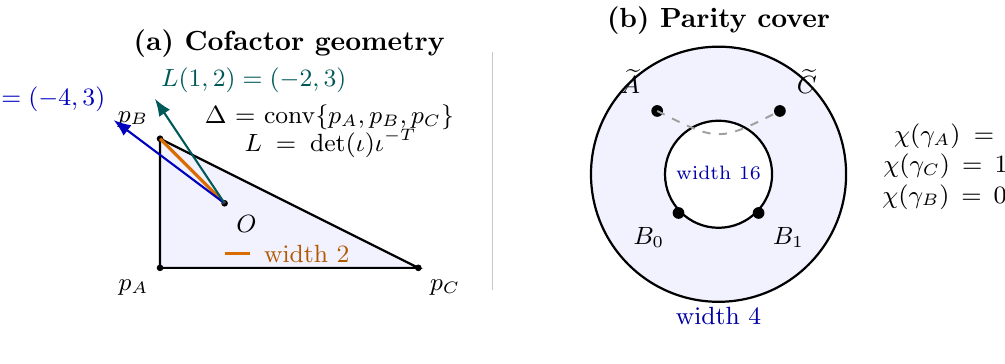
\begin{tikzpicture}[x=0.82cm,y=0.82cm,
  every node/.style={font=\small},
  focus/.style={circle,fill=black,inner sep=1.5pt},
  charge/.style={-{Latex[length=2.2mm]},line width=0.75pt},
  affine/.style={line width=0.8pt}]
  \path[use as bounding box] (-3.05,-2.05) rectangle (11.65,2.72);
  % Left panel: polygon and cofactor directions.
  \begin{scope}[shift={(0,0)}]
    \node[font=\bfseries] at (1,2.48) {(a) Cofactor geometry};
    \fill[blue!5] (-1,-1) -- (-1,1) -- (3,-1) -- cycle;
    \draw[affine] (-1,-1) -- (-1,1) -- (3,-1) -- cycle;
    \coordinate (pA) at (-1,-1);
    \coordinate (pB) at (-1,1);
    \coordinate (pC) at (3,-1);
    \coordinate (O) at (0,0);
    \fill (pA) circle (1.2pt) node[below left=1pt] {$p_A$};
    \fill (pB) circle (1.2pt) node[above left=1pt] {$p_B$};
    \fill (pC) circle (1.2pt) node[below right=1pt] {$p_C$};
    \fill (O) circle (1.2pt) node[below right=1pt] {$O$};
    \draw[orange!85!black,line width=1.15pt] (O) -- (pB);
    % legend for the highlighted star edge through the width-two point B
    \draw[orange!85!black,line width=1.15pt] (0.0,-0.78) -- (0.4,-0.78)
      node[right=1pt,text=orange!70!black] {width $2$};
    \draw[charge,blue!75!black] (O) -- ++(-1.72,1.29)
      node[above left=-1pt] {$L(2,1)=(-4,3)$};
    \draw[charge,teal!70!black] (O) -- ++(-1.08,1.62)
      node[above right=-2pt] {$L(1,2)=(-2,3)$};
    \node[align=center,text width=3.4cm] at (1.64,1.12)
      {$\Delta=\operatorname{conv}\{p_A,p_B,p_C\}$\\[-1pt]
       $L=\det(\iota)\iota^{-T}$};
  \end{scope}

  % Separator.
  \draw[gray!45] (4.15,-1.35) -- (4.15,2.35);

  % Right panel: annular parity cover; the dashed arc is a lift of the branch segment.
  \begin{scope}[shift={(7.65,0.45)}]
    \node[font=\bfseries] at (0,2.38) {(b) Parity cover};
    \fill[blue!5,even odd rule]
      (0,0) circle (1.62cm)
      (0,0) circle (0.68cm);
    \draw[affine] (0,0) circle (1.62cm);
    \draw[affine] (0,0) circle (0.68cm);
    \node[focus,label={[xshift=-1pt,yshift=1pt]above left:$\widetilde A$}] at (-0.95,0.98) {};
    \node[focus,label={[xshift=1pt,yshift=1pt]above right:$\widetilde C$}] at (0.95,0.98) {};
    \node[focus,label=below left:$B_0$] at (-0.62,-0.60) {};
    \node[focus,label=below right:$B_1$] at (0.62,-0.60) {};
    \node[blue!65!black,inner sep=1pt] at (0,-2.2) {width $4$};
    \node[blue!65!black,inner sep=1pt,font=\scriptsize] at (0,0.02) {width $16$};
    \draw[dashed,gray!75,line width=.7pt] (-0.95,0.98)
      .. controls (0,0.50) .. (0.95,0.98);
    \node[align=center,text width=2.45cm,anchor=west] at (1.85,0.12)
      {$\chi(\gamma_A)=\chi(\gamma_C)=1$\\
       $\chi(\gamma_B)=0$};
  \end{scope}
\end{tikzpicture}

\end{adjustbox}
\caption{The quartic polygon and its annular parity cover.  (a) The polygon
$\Delta$ with vertices $p_A,p_B,p_C$, in the coordinates $(s_1,s_2)$; the
highlighted star edge from $O$ to $p_B$ contains the singular point $B$,
whose monodromy has width two.  The first two singleton supports are the
cofactor directions $L(2,1)$ and $L(1,2)$.  (b) Two copies of the disk, cut
along the branch segment from $A$ to $C$, are glued crosswise; the dashed
arc is one of the two lifts of this segment.  The boundary circles have
widths $4$ and $16$.  The cover is branched over $A$ and $C$, whose
preimages are the ramification points $\widetilde A,\widetilde C$, and $B$ has two
unramified lifts $B_0,B_1$.}
\label{fig:annular-cover}
\end{figure}

The annulus $\overline\Acal$ with its $\widetilde M$-affine structure is thus
determined by the lattice $\widetilde M$ of the first descendent exponents.
Section~\ref{sec:compactification} compares it with the affine bases of
distinguished toric degenerations in the sense of \cite{carletal2024}.

\subsection{Local Kummer charts}
\label{subsec:kummer-charts}

Each matrix in \eqref{eq:lifted-monodromies} exchanges $\alpha$ and $\beta$
in $\widetilde M/M$, while the core matrix $K$ acts trivially.  The
monodromy of the local system with fiber $\widetilde M/M$ therefore acts
through the exchange of $\alpha$ and $\beta$, and $\deg_4$ of
\eqref{eq:diagonal-charge} is the projection onto its largest quotient on
which the monodromy acts trivially.  The local system becomes constant on
the connected double cover
\[
 p_{\mathrm{fr}}:\Acal^\circ_{\mathrm{fr}}\longrightarrow\Acal^\circ
\]
defined by the kernel of the monodromy action on $\widetilde M/M$.  We call
$p_{\mathrm{fr}}$ the \emph{fractional-exponent cover}: it is the smallest
connected cover on which the fractional-exponent group forms a constant
local system.  Its deck involution $\delta_{\mathrm{deck}}$ exchanges the
classes $\alpha$ and $\beta$.  The lifted slab maps require, in addition,
roots of the slab functions; these are the Kummer roots constructed below.

\emph{Placement of the transitions.}  For $V\in\{A,B,C\}$ let $c_V$ be the
outer half of the star edge through $V$, the segment from $V$ to the vertex
$p_V$ of $\Delta$.  The complement of $c_A\cup c_B\cup c_C$ in the interior
of $\Delta$ is simply connected and contains $O$, the inner half-edges and
the branch segment from $A$ to $C$.  Its preimage in $\overline\Acal$
therefore consists of two \emph{sheets} $S_0$ and $S_1$, each mapped
homeomorphically onto it; we write $O_0\in S_0$ and $O_1\in S_1$ for the two
lifts of the central vertex $O$.  The preimage of $c_B$ consists of one arc
from each $B_i$ to the boundary, and the preimages of $c_A$ and $c_C$
consist of two arcs from $\widetilde A$ and two from $\widetilde C$, one to
each boundary circle.  We call these six arcs the \emph{cuts}.  All
transitions at the singular points, namely the affine transitions, the
lifted slab maps below and the line transitions of
Section~\ref{sec:jacobi-theta}, are carried by the cuts, which run from the
singular points outward to the boundary.  The sheets carry no transition;
in particular none is carried by the inner half-edges, by the preimage of
the branch segment, or near $O_0$ and $O_1$.  By
Proposition~\ref{prop:proper-supports}, no wall support of
Section~\ref{sec:jacobi-theta} meets an arc carrying a transition.

We give $S_0$ a fixed frame and $S_1$ the continuation of that frame across the arc
over $c_A$ that $\gamma_A$ crosses from $S_0$, so that this arc carries no
transition.  We place the lifted slab map at each singular
point on a single arc from that point to the boundary: at $B_0$ and $B_1$ on
the arcs over $c_B$, at $\widetilde A$ on the arc over $c_A$ that $\gamma_A$
crosses from $S_1$, and at $\widetilde C$ on the arc over $c_C$ that
$\gamma_C$ crosses from $S_1$.  The arc over $c_C$ that $\gamma_C$ crosses
from $S_0$ carries only the change of affine chart along
$\gamma_{\mathrm{core}}$.  As in Appendix~\ref{app:calculations}, a product
$gh$ of loops traverses $g$ first.  Thus $\gamma_{\mathrm{core}}=\gamma_C\gamma_A^{-1}$
crosses only the arc carrying the change of chart and the arc carrying no
transition, and the transport along it has linear part $K$ and no slab
factor.  The dual graph of this decomposition is the Schreier graph of the
parity subgroup for the transversal $\{1,\gamma_A\}$, and its five edges
other than the transversal edge correspond to the generators
\eqref{eq:parity-matrices}.

\emph{Chart algebras.}  Every vertex of the path tree $\Tcal$ of
Section~\ref{subsec:root-orbit}, a reduced edge path from $S_0$ to a sheet,
carries the frame obtained from that of $S_0$ by transport along the path;
the frames of $S_0$ and $S_1$ fixed above are those at the empty path and at
the path that crosses the arc over $c_A$ carrying no transition.  The
\emph{chart algebra} of a sheet, or of a point or a region of $\Acal^\circ$
read in the frame at a vertex, is $\Bbbk[\widetilde M]$ in that frame, over
the Kummer ring of the relevant finite stage: for a finite rooted subtree
$T\subset\Tcal$ containing the vertex, it is the Kummer ring
$R_T^{\mathrm{root}}$ of \eqref{eq:finite-kummer-ring}, into which
$\Bbbk[\widetilde M]$ in that frame maps by pull-back along the path of the
vertex (Section~\ref{subsec:root-stage-regularity}), tensored with the
coefficient ring in use, such as $R/\mathfrak m^N$ in
\eqref{eq:annular-root-object} or a truncated coefficient ring of
Section~\ref{sec:compactification}.

For $V\in\{\widetilde A,B_0,B_1,\widetilde C\}$ let $u_V\in\widetilde M$ be
the primitive vector spanning the invariant line of $H_V$, and let
$x_V=z^{2\epsilon_Vu_V}$ with the signs $\epsilon_V$ below.  The exponent
$2\epsilon_Vu_V$ is the invariant character $\bar u_V\in M$ of the disk
monodromy $T_V$ about the image of $V$, that is, one of the characters
$\bar u_A,\bar u_B,\bar u_C$ of $T_A,T_B,T_C$ listed in
Appendix~\ref{app:calculations}, transported linearly along $\gamma_A$ for
$B_1$.  The pulled-back slab functions are
\[
 f_{\widetilde A}=1+x_{\widetilde A},\qquad
 f_{B_i}=1+a_\rho x_{B_i}+x_{B_i}^2,\qquad
 f_{\widetilde C}=1+x_{\widetilde C},
\]
of degree $e_V=1,2,2,1$ in $x_V$.  Let $N_V\in\widetilde M^\vee$ be the
primitive conormal of the invariant line, with the sign fixed by
\begin{equation}\label{eq:monodromy-sign}
 H_V-\mathrm{Id}=-\frac{e_V}{d_V}\,(2\epsilon_Vu_V)\,N_V^{T}=-\epsilon_V\,u_VN_V^T,
\end{equation}
where $d_V$ is the root degree below.  The data, with $u_V$ and $N_V$ given
by their $F$-coordinates, are
\begin{equation}\label{eq:root-data}
\begin{array}{c|cccc}
 V&\widetilde A&B_0&B_1&\widetilde C\\ \hline
 F^{-1}u_V&(3,1)&(1,-1)&(5,3)&(1,3)\\
 \epsilon_V&1&1&-1&-1\\
 d_V&2&4&4&2\\
 F^{T}N_V&(1,-3)&(-1,-1)&(-3,5)&(-3,1).
\end{array}
\end{equation}
On the complement of the slab divisor put
\begin{equation}\label{eq:local-root-ring}
 R_V^{\mathrm{root}}
 =\Bbbk[\widetilde M][f_V^{-1},g_V]/(g_V^{d_V}-f_V),
 \qquad
 \widetilde\theta_V(z^m)=g_V^{\langle N_V,m\rangle}z^m.
\end{equation}
The ring $R_V^{\mathrm{root}}$ is the Kummer ring of $f_V$.  Its spectrum is
the restriction, over the complement of the slab divisor, of the Kummer
cover $\Spec\Bbbk[\widetilde M][g_V]/(g_V^{d_V}-f_V)$, whose quotient by
$\mu_{d_V}$, acting by $g_V\mapsto\zeta g_V$ and trivially on characters, is
the $d_V$th root stack of the slab divisor (Appendix~\ref{app:calculations}).
Over the complement of the divisor the Kummer cover is a
$\mu_{d_V}$-torsor, the root stack is the complement itself, and $g_V$ is not
a function on it.  Since $\langle N_V,u_V\rangle=0$, the map
$\widetilde\theta_V$ fixes $f_V$ and $g_V$ and is an automorphism of
$R_V^{\mathrm{root}}$.  It commutes with $\mu_{d_V}$ on $z^m$ exactly when
$d_V$ divides $\langle N_V,m\rangle$.  This holds for $m\in M$, where
$\langle N_V,m\rangle\in4\ZZ$ and $\widetilde\theta_V$ multiplies $z^m$ by an
integral power of $f_V$, and it fails for some $m\in\widetilde M$ because
$N_V$ is primitive.  The lifted slab maps, the line transitions of
Section~\ref{sec:jacobi-theta} and every transport built from them therefore
act on Kummer rings and Kummer covers, and not on root stacks.

The lifted slab map at $V$ is placed on its arc so that the transport along
the loop $\gamma_V$ of Section~\ref{subsec:parity-cover}, based in $S_0$, is
$z^m\mapsto g_V^{\langle N_V,m\rangle}z^{H_Vm}$.  By
\eqref{eq:monodromy-sign}, $z^{H_Vm}=z^{m-\epsilon_V\langle N_V,m\rangle u_V}$,
and $g_V^{d_V}x_V^{-e_V}=f_Vx_V^{-e_V}$ tends to one where $x_V$ is large;
in this sense the transport is trivial to leading order there, which fixes
the sign of $N_V$.

\begin{proposition}\label{prop:minimal-roots}
The formula \eqref{eq:local-root-ring} defines an automorphism of the Kummer
ring $R_V^{\mathrm{root}}$ extending the transition of the disk: on
characters $m\in M$, the transports about $\widetilde A$, $B_0$ and $\widetilde C$
based in $S_0$ are the disk transports about $A$ twice, $B$ once and $C$
twice, and the transport about $B_1$ is the disk transport about $B$ written
in the frame of $S_1$.  For $a_\rho\neq\pm2$ the root degrees $2,4,4,2$ are
minimal.
\end{proposition}

\begin{proof}
The root $g_V$ is a unit on the localized chart and
$\langle N_V,m\rangle$ is integral.  Moreover $N_V=4n_V$, where
$n_V\in M^\vee$ is the primitive conormal of the disk at the image of $V$,
transported linearly along $\gamma_A$ for $B_1$; the arc that $\gamma_A$
crosses from $S_0$ carries no transition.  The disk transport about that
singular point is $z^m\mapsto f_V^{\langle n_V,m\rangle}z^{T_Vm}$, where
$T_V-\mathrm{Id}=-e_V\bar u_Vn_V^T$ by \eqref{eq:disk-rank-one}; at $B_1$, the slab function, the invariant
character, the conormal and the monodromy are those of $B$ transported
linearly along $\gamma_A$, that is, written in the frame of $S_1$.  The disk
transport fixes $f_V$ and $n_V$.  At $\widetilde A$ and $\widetilde C$ the
loop traverses the disk loop twice, so on $m\in M$ the slab factor is
$f_V^{2\langle n_V,m\rangle}=g_V^{\langle N_V,m\rangle}$; at $B_0$ and $B_1$
it traverses it once, giving $f_V^{\langle n_V,m\rangle}=g_V^{\langle
N_V,m\rangle}$.  Since $N_V$ is primitive, $\langle N_V,m\rangle=1$ for some
$m\in\widetilde M$, so the slab factor of that character is a $d_V$th root
of $f_V$.  For $a_\rho\neq\pm2$ the Laurent polynomial $f_V$ vanishes to order
one along each component of its zero divisor, so its class in
$\Bbbk(\widetilde M)^\times/\Bbbk(\widetilde M)^{\times d_V}$ has order
$d_V$, and no proper divisor of $d_V$ suffices.
\end{proof}

The placement above thus defines the lifted coefficient system.  On
characters in $M$ it agrees with the pullback of the disk system germwise at
each singular point (Proposition~\ref{prop:minimal-roots}), but it is not
that pullback.  In the pulled-back system each of the two arcs over $c_A$,
and each of the two over $c_C$, carries the disk transition, whose slab
factor on a single crossing is $f_V^{\langle n_V,m\rangle}$ with
$\langle n_V,m\rangle\in\frac14\ZZ$ for $m\in\widetilde M$.  On characters in
$M$, the pulled-back disk transport along $\gamma_A\gamma_B\gamma_A^{-1}$ is
the transport about $B_1$ conjugated by
$z^m\mapsto f_A^{\langle n_A,m\rangle}z^m$, and the pulled-back transport
along $\gamma_{\mathrm{core}}$ has slab factors, powers of $f_C$ and of the
transport of $f_A$, whereas the transport of the lifted system along
$\gamma_{\mathrm{core}}$ is the monomial map with linear part $K$.

At the two cusps $a_\rho=\pm2$ the degree at $B_0$ and $B_1$ drops to two.  If
$f_B(a_\rho,z)=1+a_\rho z+z^2$, then
\begin{equation}\label{eq:cusp-roots}
\begin{aligned}
 a_\rho=2:&\quad g^4-f_B=(g^2-(1+z))(g^2+(1+z)),\\
 a_\rho=-2:&\quad g^4-f_B=(g^2-(1-z))(g^2+(1-z)).
\end{aligned}
\end{equation}
Away from the reduced zero divisor these are two connected quadratic
torsors; their closures meet over the divisor.  We retain this fourth-root
stack rather than replacing it by one connected square-root cover.

\subsection{The infinite root orbit}
\label{subsec:root-orbit}

The failure of finite Kummer closure already occurs on the overlap of the
$\widetilde A$ and $B_0$ charts.  Write
\[
 x_A=x_{\widetilde A}=z^{2u_{\widetilde A}},\qquad
 x_B=x_{B_0}=z^{2u_{B_0}},\qquad f_A=1+x_A,\qquad
 f_B(x)=1+a_\rho x+x^2,
\]
and let $\mathcal K=\Bbbk(x_A,x_B)$.  Since
$\langle N_{\widetilde A},2u_{B_0}\rangle=8$ and $d_{\widetilde A}=2$, the
$\widetilde A$-slab shear fixes $f_A$ and sends
\begin{equation}\label{eq:shear}
 x_B\longmapsto f_A^4x_B.
\end{equation}
The transport about $\widetilde A$ also applies the linear monodromy, and
$H_A(2u_{B_0})=2u_{B_0}-4\cdot2u_{\widetilde A}$; it therefore fixes $x_A$
and sends $x_B$ to $x_A^{-4}f_A^4x_B=(1+x_A^{-1})^4x_B$.  For $a_\rho\neq\pm2$
write $f_B(x)=(1+\lambda x)(1+\lambda^{-1}x)$ with $\lambda+\lambda^{-1}=a_\rho$
and $\lambda^2\neq1$.

\begin{theorem}[Infinite Kummer orbit]\label{thm:infinite-root-orbit}
Let $u\in\Bbbk(x_A)$ be nonconstant, and let $\omega_u$ be the automorphism
of $\mathcal K$ fixing $x_A$ with $\omega_u(x_B)=ux_B$.  The slab shear
\eqref{eq:shear}, with $u=f_A^4$, and the transport about $\widetilde A$,
with $u=(1+x_A^{-1})^4$, are of this form.
\begin{enumerate}
\item If $a_\rho\neq\pm2$, closure of a fourth root of $f_B(x_B)$ under all
powers of $\omega_u$ requires the fourth roots $g_n$ of
\begin{equation}\label{eq:root-tower}
 g_n^4=f_B(u^nx_B)
 =\bigl(1+\lambda u^nx_B\bigr)\bigl(1+\lambda^{-1}u^nx_B\bigr),
 \qquad n\in\ZZ,
\end{equation}
and the classes of these radicands are linearly independent over $\ZZ/4$ in
$\mathcal K^\times/\mathcal K^{\times4}$.
\item If $a_\rho=\pm2$, then $f_B(u^nx_B)=(1\pm u^nx_B)^2$, and the classes of
$1\pm u^nx_B$, $n\in\ZZ$, are linearly independent over $\ZZ/2$ in
$\mathcal K^\times/\mathcal K^{\times2}$.
\item In either case no finite extension of $\mathcal K$ containing a fourth root
of $f_B(x_B)$ admits an automorphism extending $\omega_u$.  In particular no
finite algebraic Kummer extension containing the initial $\widetilde A$- and
$B_0$-roots is stable under the slab shear or under transport about
$\widetilde A$.
\end{enumerate}
\end{theorem}

\begin{proof}
Suppose $a_\rho\neq\pm2$.  In the principal ideal domain $\Bbbk(x_A)[x_B]$,
\[
 f_B(u^nx_B)
 =u^{2n}\bigl(x_B+\lambda^{-1}u^{-n}\bigr)\bigl(x_B+\lambda u^{-n}\bigr).
\]
The elements $\lambda^{\pm1}u^{-n}$, $n\in\ZZ$, of $\Bbbk(x_A)$ are pairwise
distinct: an equality $\lambda^{\epsilon}u^{-n}=\lambda^{\epsilon'}u^{-m}$
makes $u^{m-n}$ constant, hence $m=n$ because $u$ is nonconstant, and then
$\lambda^{\epsilon}=\lambda^{\epsilon'}$ forces $\epsilon=\epsilon'$ because
$\lambda^2\neq1$.  Thus $\pi_n=x_B+\lambda^{-1}u^{-n}$ is a prime dividing the
$n$th radicand exactly once and no other radicand.  If a finite product
$\prod_nf_B(u^nx_B)^{k_n}$ is a fourth power in $\mathcal K$, its $\pi_n$-adic
valuation $k_n$ is divisible by four.  This proves (1).  For (2), the same
argument applies to the primes $x_B\pm u^{-n}$ of $1\pm u^nx_B$.

For (3), let $\mathcal K'\supset\mathcal K$ be finite, let $\widetilde\omega$ be an
automorphism of $\mathcal K'$ extending $\omega_u$, and let $h\in\mathcal K'$ satisfy
$h^4=f_B(x_B)$.  Then $\widetilde\omega^n(h)^4=f_B(u^nx_B)$ for every
$n\in\ZZ$.  If $a_\rho\neq\pm2$, the field $\Bbbk$ contains the fourth roots of
unity, so by Kummer theory and (1) the subfield generated by the
$\widetilde\omega^n(h)$ with $|n|\leq r$ has degree $4^{2r+1}$ over $\mathcal K$
for every $r$, which is impossible.  If $a_\rho=\pm2$, then
$\widetilde\omega^n(h)^2=\pm(1\pm u^nx_B)$, and since $-1$ is a square in
$\Bbbk$, $\mathcal K'$ contains square roots of all $1\pm u^nx_B$; by (2) the same
degree argument applies with $2^{2r+1}$.
\end{proof}

\emph{The path tree.}  Let $\mathfrak C$ be the graph whose vertices are the
two sheets $S_0,S_1$ and whose edges are the six cuts, each joining the
sheets on its two sides.  The sheets are simply connected and the cuts are
contractible, so the fundamental group of $\mathfrak C$ based at $S_0$ is
$\Pi=\pi_1(\Acal^\circ)$, a free group of rank five.  The \emph{path tree}
$\Tcal$ is the universal covering tree of the graph $\mathfrak C$.  Its
vertices are the reduced edge paths in $\mathfrak C$ beginning at $S_0$,
equivalently the homotopy classes of paths in $\Acal^\circ$ from a base
point $b_0\in S_0$ to $b_0$ or to the other lift $b_1\in S_1$ of its image
in $\Delta$; its root is the empty path at $S_0$.

Let $\mathbb T=\Spec\Bbbk[\widetilde M]$ be the torus of the sheet $S_0$, and let
$T\subset\Tcal$ be a finite rooted subtree.  We call an edge of $T$ a
\emph{Kummer edge} if it crosses, in either direction, an arc carrying a
lifted slab map; edges crossing the other two arcs adjoin no root.
Number the Kummer edges $e=1,\dots,\ell$, the edge $e$ crossing the arc of the
singular point $V_e$.  It has the root degree $d_e=d_{V_e}$ and the
\emph{transported radicand} $\varrho_e$, the transport of $f_{V_e}$ to $S_0$
along the path of $T$ preceding $e$.  The vectors $u_V$ lie in the
sublattice of $\widetilde M$ of elements whose $F$-coordinates $(m_1,m_2)$
satisfy $m_1\equiv m_2\pmod2$, which the matrices
\eqref{eq:parity-matrices} preserve and on which every $N_V$ is even.  A
lifted slab map therefore multiplies a transported character
$z^{2\epsilon_{V'}u_{V'}}$ by a power of the root it uses with exponent
divisible by four, that is, by an integral power of the corresponding
transported radicand.  By induction along the path, every $\varrho_e$ is a
rational function on $\mathbb T$.  Let $U_T\subset\mathbb T$ be the complement of the zeros
and poles of $\varrho_1,\dots,\varrho_\ell$, and put
$G_T=\prod_e\mu_{d_e}$.  The \emph{Kummer ring} of $T$ is
\begin{equation}\label{eq:finite-kummer-ring}
 R_T^{\mathrm{root}}
 =\mathcal O(U_T)[r_1,\dots,r_\ell]\big/\bigl(r_e^{d_e}-\varrho_e\bigr)_{e},
\end{equation}
on which $\zeta\in G_T$ acts by $r_e\mapsto\zeta_er_e$.  It is finite étale
over $\mathcal O(U_T)$, and $\Spec R_T^{\mathrm{root}}$ is a $G_T$-torsor
over $U_T$.  The lifted slab map at the Kummer edge $e$ uses the root $r_e$,
the transport of $g_{V_e}$, so transport along the paths of $T$ is defined
on $R_T^{\mathrm{root}}$.  Let $D_e$ be the divisor of zeros of
$\varrho_e$ on $\mathbb T$.  The \emph{finite root stack} of $T$ is
\[
 \Xfrak_T=\sqrt[d_1]{(\mathbb T,D_1)}\times_{\mathbb T}\cdots\times_{\mathbb T}\sqrt[d_\ell]{(\mathbb T,D_\ell)},
\]
in the convention \eqref{eq:root-stack-chart-app}.  Over $U_T$ it is $U_T$
itself, the quotient of $\Spec R_T^{\mathrm{root}}$ by $G_T$.
Section~\ref{sec:compactification} extends $\Spec R_T^{\mathrm{root}}$ to a
Kummer cover $P_T$ of $\mathbb T$ with $\Xfrak_T=[P_T/G_T]$; we call $\Xfrak_T$ with
its atlas $P_T$ the \emph{finite root-stack presentation} of $T$.
Transport acts on $R_T^{\mathrm{root}}$, that is, on $P_T$ over $U_T$, and
not on $\Xfrak_T$, because the lifted slab maps do not commute with $G_T$.
By Appendix~\ref{app:calculations}, the stabilizer of $\Xfrak_T$ at a
geometric point over $z\in\mathbb T$ is the product of the factors
$\mu_{d_e}$ with $z\in D_e$.  If $T\subset T'$, localization
followed by adjunction of the new roots maps $R_T^{\mathrm{root}}$
injectively to $R_{T'}^{\mathrm{root}}$, and forgetting the new roots gives
$\Xfrak_{T'}\to\Xfrak_T$.  The paths $\gamma_{\widetilde A}^n$ followed by a
crossing of the $B_0$-arc give the radicands $f_B(u^nx_B)$,
$u=(1+x_A^{-1})^4$, of Theorem~\ref{thm:infinite-root-orbit}.

\begin{definition}\label{def:pathwise-root-object}
Let $R=\Bbbk[t_1,t_2]$ be the deformation coefficient algebra, where
$t_1,t_2$ are the singleton parameters, and let $\mathfrak m=(t_1,t_2)$ be the
singleton ideal.  The \emph{pathwise Kummer ring} is
$R_{\mathrm{path}}^{\mathrm{root}}=\varinjlim_{T\subset\Tcal}R_T^{\mathrm{root}}$,
the colimit over the finite rooted subtrees $T\subset\Tcal$.
The pathwise root object and its adic completion are the formal systems
\begin{equation}\label{eq:pathwise-root-object}
 \Xfrak_{\mathrm{path}}=\varprojlim_{T\subset\Tcal}\Xfrak_T,
 \qquad
 \widehat\Xfrak_{\mathrm{path}}
 =\varinjlim_N\varprojlim_{T\subset\Tcal}
  \bigl(\Xfrak_T\times\Spec R/\mathfrak m^N\bigr).
\end{equation}
The group $\Pi$ acts on $\Tcal$ by deck transformations, a loop acting by
concatenation, and through transport on $R_{\mathrm{path}}^{\mathrm{root}}$,
the Kummer root of an edge going to the Kummer root of its translate.  The
\emph{annular coefficient system} is $\widehat\Xfrak_{\mathrm{path}}$
together with this action of $\Pi$.  A structure over it, such as a module,
an algebra, a bracket or a wall structure, is a $\Pi$-equivariant compatible
system of such structures over the rings
\begin{equation}\label{eq:annular-root-object}
 R_T^{\mathrm{root}}\otimes_\Bbbk R/\mathfrak m^N,
 \qquad T\subset\Tcal\ \text{a finite rooted subtree},\quad N\geq1.
\end{equation}
The coefficient ring at every vertex of $\Tcal$ is
$R_{\mathrm{path}}^{\mathrm{root}}\otimes_\Bbbk R$, transport along the path
of the vertex identifying it with the ring at the empty path.  A
\emph{finite transport diagram modulo $\mathfrak m^N$} is a finite diagram of
finitely presented modules or algebras over the coefficient rings of
finitely many vertices of $\Tcal$, reduced modulo $\mathfrak m^N$, together with
finitely many homomorphisms, transports along edges of $\Tcal$, and
identities among their composites.
\end{definition}

The limit over $T$ is formed along the root-forgetting maps, the colimit of
Kummer rings along the injections $R_T^{\mathrm{root}}\to R_{T'}^{\mathrm{root}}$,
and the colimit over $N$ along the closed immersions
$\Spec R/\mathfrak m^N\to\Spec R/\mathfrak m^{N+1}$.  The limits are formal systems: by
Theorem~\ref{thm:forced-category}, $\Xfrak_{\mathrm{path}}$ is not
represented by a formal scheme or by an algebraic stack whose diagonal is
locally of finite type.  The group $\Pi$ acts on the Kummer rings,
preserving the root degrees, but not on the root stacks $\Xfrak_T$, whose
root groups $G_T$ do not commute with the lifted slab maps.  For this reason
no quotient by $\Pi$ is formed: structures over the annular coefficient
system are defined through the Kummer rings \eqref{eq:annular-root-object}
and the action of $\Pi$ on them.  This inverse system is of the same
formal kind as the infinite root stacks of \cite{talpovistoli2018}; the
additional feature here is that the roots are indexed by reduced transport
paths and permuted by the deck group $\Pi$.  Wall structures over this
object and their consistency are the subject of
Section~\ref{sec:jacobi-theta}.

\begin{theorem}[Finite-stage definability and nonrepresentability]
\label{thm:forced-category}
Every finite transport diagram modulo $\mathfrak m^N$ is defined over
$R_T^{\mathrm{root}}\otimes_\Bbbk R/\mathfrak m^N$ for some finite rooted subtree $T$,
that is, over $U_T$ on the Kummer cover $P_T$ of the finite root-stack
presentation of $T$.  Any two such subtrees have a common finite refinement.
On the other hand, if all transported roots and their automorphisms are
retained, the pathwise root object $\Xfrak_{\mathrm{path}}$ is not
represented by a formal scheme, a finite root stack, or an algebraic stack
whose diagonal is locally of finite type.
\end{theorem}

\begin{proof}
A finite transport diagram involves finitely many vertices of $\Tcal$ and,
modulo $\mathfrak m^N$, finitely many deformation bidegrees.  The rooted union of the
corresponding paths is a finite subtree.  The ring
$R_{\mathrm{path}}^{\mathrm{root}}$ is the colimit of the Kummer rings of the
finite subtrees (Appendix~\ref{app:calculations}), so by finite
presentation the finitely many generators, relations, arrows and identities
are defined over one of them after a further finite enlargement.  Rooted union gives a common
refinement.

For the negative assertion, let $u=(1+x_A^{-1})^4$, let $\lambda$ be a root
of $\lambda^2-a_\rho\lambda+1$ (so $\lambda=\pm1$ when $a_\rho=\pm2$), and let $w$ be a
geometric point of $\mathbb T$ with $x_A=-\frac12$ and $x_B=-\lambda^{-1}$.  There
$f_A=\frac12$ and $u=1$, so every radicand $f_B(u^nx_B)$ in
\eqref{eq:root-tower} vanishes.  For a finite set $S\subset\ZZ$, let $T$ be
the rooted union of the paths $\gamma_{\widetilde A}^n$ followed by a
crossing of the $B_0$-arc, $n\in S$.  Since the transport about
$\widetilde A$ fixes $f_A$, every root adjoined along
$\gamma_{\widetilde A}^n$ has the radicand $f_A$, which does not vanish at
$w$.  The root adjoined at the final crossing has the radicand
$\varrho_n=f_B(u^nx_B)$, which is regular at $w$, because $x_A$ and $f_A$ are units
there, and vanishes at $w$; hence $w\in D_n$.  The stabilizer of
$\Xfrak_T$ at the point over $w$ is therefore $\prod_{n\in S}\mu_4$.
The automorphism group of a compatible point of $\Xfrak_{\mathrm{path}}$ over
$w$ is the inverse limit of the stabilizers over all finite subtrees, and it
contains
\[
 \prod_{n\in\ZZ}\mu_4
\]
as a closed subgroup.  This group scheme is not of finite type.  A formal
scheme has trivial stabilizers, a finite root stack has finite-type
diagonal, and an algebraic stack with diagonal locally of finite type cannot
have such a geometric stabilizer.
\end{proof}

Theorem~\ref{thm:forced-category} is the only property of the inverse
system used later: every product, period and logarithmic chart below is
constructed over the Kummer ring of a finite stage, and the pro-object
records the compatibility of these constructions.

\section{Jacobi scattering and theta functions}
\label{sec:jacobi-theta}

\subsection{The twisted volume line}

Fix a root chamber and an integral basis $e_1,e_2$ of $\widetilde M$.  Put
\begin{equation}\label{eq:primitive-form}
 \kappa=e_1+e_2,
 \qquad \Omega_0=d\log z_1\wedge d\log z_2,
 \qquad \Omega_\kappa=z^\kappa\Omega_0.
\end{equation}
Let $J(q_1,q_2)=(q_2,-q_1)$ and denote the invariant logarithmic derivation
in direction $v$ by $\partial_v$.

\begin{proposition}[Shifted Hamiltonian bracket]
\label{prop:shifted-bracket}
The inverse bivector $\pi_\kappa=z^{-\kappa}\pi_0$ of $\Omega_\kappa$ has
Hamiltonian vector fields
\begin{equation}\label{eq:shifted-Hamiltonian}
 X_q^\kappa=z^{q-\kappa}\partial_{Jq},
\end{equation}
and
\begin{equation}\label{eq:shifted-bracket}
 [X_q^\kappa,X_r^\kappa]
 =-\det(q,r)X_{q+r-\kappa}^\kappa.
\end{equation}
Thus, after writing $q=k+\kappa$ and $r=\ell+\kappa$, the output is indexed
by $k+\ell$.
\end{proposition}

\begin{proof}
The Hamiltonian field of $z^q$ for $z^{-\kappa}\pi_0$ is
\eqref{eq:shifted-Hamiltonian}.  The bracket of two monomial derivations has
direction
\[
 \langle Jq,r-\kappa\rangle Jr
 -\langle Jr,q-\kappa\rangle Jq
 =-\det(q,r)J(q+r-\kappa),
\]
which gives \eqref{eq:shifted-bracket}.
\end{proof}

The lifted slab map at $V$ is symplectic for $\Omega_0$, but
\begin{equation}\label{eq:slab-conformal}
 \widetilde\theta_V^*\Omega_\kappa
 =g_V^{\langle N_V,\kappa\rangle}\Omega_\kappa,
 \qquad
 \bigl(\langle N_V,\kappa\rangle\bigr)_V=(-2,-2,2,-2).
\end{equation}
Choose a local line frame $e$ and identify frames across the slab by
\begin{equation}\label{eq:line-transition}
 \widetilde\theta_V^*e'=g_V^{-\langle N_V,\kappa\rangle}e.
\end{equation}
The products $\Omega_\kappa\otimes e$ then glue.  We denote the resulting
line by $\Lcal_\kappa$.

The transition law therefore requires a line bundle.

\begin{proposition}[No scalar frame]\label{prop:no-scalar-frame}
The scalar $\kappa$-twisted Hamiltonian algebra containing the two singleton
fields is not preserved under conjugation by any lifted slab transition.
Consequently its local brackets do not glue to a bracket on the structure
sheaf.
\end{proposition}

\begin{proof}
If $p_V$ is the slab exponent and
\[
 S_V=\frac1{d_V}\log(1+z^{p_V})\partial_{N_V},
\]
then for $k=q-\kappa$ one computes
\begin{equation}\label{eq:mixed-slab-bracket}
 [S_V,X_q^\kappa]
 =\sum_{r\geq1}\frac{(-1)^{r+1}}{d_V}z^{k+rp_V}
 \left(
  \frac{\langle N_V,k\rangle}{r}\partial_{Jq}
  -\langle Jq,p_V\rangle\partial_{N_V}
 \right).
\end{equation}
With respect to $\Omega_\kappa$, the divergence of the $r$th summand has
coefficient
\[
 \frac{(-1)^r}{d_V}
 \langle Jq,p_V\rangle\langle N_V,\kappa\rangle.
\]
For $r=1$ and the singleton exponents $q_1=(2,1)$ and $q_2=(1,2)$, the
eight coefficients are
\[
\begin{array}{c|rrrr}
 &A&B_0&B_1&C\\ \hline
 q_1&2&3&1&-10\\
 q_2&10&3&-7&-2.
\end{array}
\]
Thus every singleton--slab interaction has nonzero divergence.
\end{proof}

\begin{proposition}[Jacobi transport]\label{prop:Jacobi-transport}
The line $\Lcal_\kappa$ on the pathwise pro-root object carries a canonical
Jacobi bracket whose expression in the distinguished chamber is the
$\kappa$-twisted Poisson bracket.  Every lifted slab transition is a Jacobi
isomorphism.  The construction is compatible with finite root restriction
and descends with the pro-Kummer coefficient object.
\end{proposition}

\begin{proof}
In a frame $e$, write a Jacobi bracket as
\[
 \{fe,he\}=
 \bigl(\Lambda(df,dh)+fE(h)-hE(f)\bigr)e.
\]
Under $e'=ae$ the local pair transforms by
\begin{equation}\label{eq:Jacobi-frame-change}
 \Lambda'=a\Lambda,
 \qquad E'=aE+\Lambda^\sharp(da).
\end{equation}
Start at the root chamber with $(\Lambda,E)=(\pi_\kappa,0)$ and transport
the pair across each edge using \eqref{eq:line-transition} and
\eqref{eq:Jacobi-frame-change}.  Every vertex of the path tree has a unique
route from the root, so the construction is unambiguous and compatible with
restriction to finite subtrees.  Change of frame and pullback preserve the
Jacobi identity.  The deck action transports the same data, giving descent.
\end{proof}

Equivalently, $\Lcal_\kappa^\vee\setminus0$ carries the Poissonization of
this Jacobi structure.  The line-bundle formulation displays the slab
multiplier in \eqref{eq:line-transition} explicitly.

\begin{definition}[Jacobi walls and consistency]\label{def:Jacobi-wall}
Fix a finite root-stack presentation and reduce the coefficient ring modulo $I^N$.  A
\emph{Jacobi wall} is a pair $(\mathfrak d,\Theta_{\mathfrak d})$, where
$\mathfrak d$ is an oriented rational affine segment, ray, or full chord in
the smooth locus and $\Theta_{\mathfrak d}$ is a locally constant
unipotent Jacobi automorphism along $\mathfrak d$, congruent to the identity
modulo $I$.  The automorphism is read in the local frame of
$\Lcal_\kappa$ and is transported between wall charts by
Proposition~\ref{prop:Jacobi-transport}.

For a transverse path $\gamma$, its \emph{path-ordered product}
$\Theta_\gamma$ is the product of the crossed wall automorphisms in crossing
order, using the inverse when the coorientation is reversed.  A locally
finite collection of Jacobi walls is \emph{consistent at a joint} if the
path-ordered product around a sufficiently small positively oriented loop
about that joint is the identity.  It is \emph{contractibly consistent} if
$\Theta_\gamma$ depends only on the homotopy class of $\gamma$ relative to
its endpoints for homotopies through compact transverse paths.
\end{definition}

All these notions are finite-stage notions.  A wall structure on the
pro-Kummer object means a compatible system of such structures as the root
stage and $N$ vary.  This convention prevents inverse-limit notation from
hiding an infinite path-ordered product.

\subsection{The singleton joint}

Let $t_1,t_2$ be the two singleton parameters, $I=(t_1,t_2)$, and put
\begin{equation}\label{eq:singleton-generators}
 E_{a,b}=t_1^at_2^bX_{\kappa+(a,b)}^\kappa,
 \qquad (a,b)\in\NN^2\setminus\{(0,0)\}.
\end{equation}
Then
\begin{equation}\label{eq:singleton-bracket}
 [E_{a,b},E_{c,d}]
 =-\det\bigl(\kappa+(a,b),\kappa+(c,d)\bigr)E_{a+c,b+d}.
\end{equation}
The two incoming GKT normalizations are
\begin{equation}\label{eq:incoming-singletons}
 \mathsf A=-\frac12E_{1,0},
 \qquad \mathsf B=-\frac12E_{0,1}.
\end{equation}
Since the shifted exponents are $(2,1)$ and $(1,2)$,
\begin{equation}\label{eq:first-bracket}
 [\mathsf A,\mathsf B]= -\frac34E_{1,1}.
\end{equation}

\begin{proposition}[Ordered singleton completion]
\label{prop:singleton-completion}
Let $\widehat{\mathfrak g}_{\mathrm{sing}}$ be the product of the lines
spanned by the $E_{a,b}$, completed in total deformation degree.  The
inverse commutator
\begin{equation}\label{eq:singleton-commutator}
 \bigl(e^{\mathsf A}e^{\mathsf B}e^{-\mathsf A}e^{-\mathsf B}\bigr)^{-1}
\end{equation}
has a unique factorization into ray groups in increasing shifted slope.  The
factorization is finite modulo $I^N$, is compatible under reduction of $N$,
and begins with $\exp(\frac34E_{1,1})$ in the chosen outgoing orientation.
\end{proposition}

\begin{proof}
Formula~\eqref{eq:singleton-bracket} gives an $\NN^2$-grading with finitely
many components modulo $I^N$.  Generators whose shifted exponents lie on one
ray commute.  At each total degree, take the logarithm of the residual word,
decompose its homogeneous part into ray summands, and insert the summands in
slope order.  This is the standard filtered factorization for
two-dimensional scattering diagrams \cite{grosspandharipandesiebert2010}.
Directness of the ray decomposition gives uniqueness.  Equation
\eqref{eq:first-bracket} gives the initial coefficient and the inverse-loop
sign.
\end{proof}

\subsection{Cofactor supports and consistency}

In the plus cofactor chart, the incoming shifted exponents have support
directions
\begin{equation}\label{eq:cofactor-singletons}
 L(2,1)=(-4,3),
 \qquad L(1,2)=(-2,3).
\end{equation}
Each is placed on the full chord through the central point $O$.  Full chords
are forced: a small loop around the endpoint of a truncated degree-one wall
would cross that wall once, while every correction begins in degree two.

If $q=\lambda(2,1)+\mu(1,2)$ with $\lambda,\mu\geq0$, then
\begin{equation}\label{eq:outgoing-cofactor}
 Lq=(-4\lambda-2\mu,3\lambda+3\mu).
\end{equation}
For $\lambda>\mu$ the ray exits one upper facet, for $\mu>\lambda$ it exits
the other, and for $\lambda=\mu$ it runs to the $B$ singularity.  A
correction parallel to an incoming ray is multiplied into the positive half
of the same chord.  Every other correction is placed on its own outgoing
radial support.

\begin{figure}[t]
\centering
\begin{adjustbox}{max width=\textwidth,center}
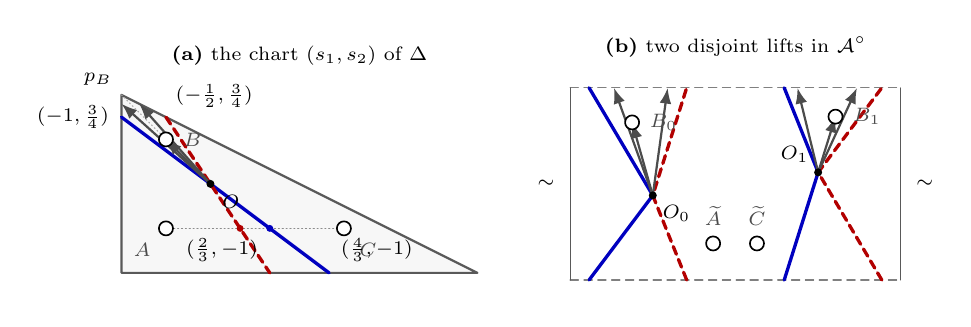
\begin{tikzpicture}[
  line cap=round,
  line join=round,
  >=Latex,
  every node/.style={font=\scriptsize},
  singletonone/.style={blue!75!black,very thick},
  singletontwo/.style={red!70!black,very thick,densely dashed},
  completion/.style={black!70,thick,-{Latex[length=2mm]}},
  branch/.style={black!45,densely dotted},
  focus/.style={circle,draw=black,fill=white,inner sep=1.8pt,line width=.6pt}
]
% Bounding box.
\draw[white] (-1.35,-1.45) rectangle (8.95,1.75);
% (a) The chart of Delta.
\begin{scope}[x=1.13cm,y=1.13cm]
  \coordinate (pA) at (-1,-1);
  \coordinate (pB) at (-1,1);
  \coordinate (pC) at (3,-1);
  \coordinate (O) at (0,0);
  \fill[black!3] (pA)--(pB)--(pC)--cycle;
  \draw[black!65,thick] (pA)--(pB)--(pC)--cycle;

  \draw[branch] (-.5,-.5)--(1.5,-.5);
  \node[focus,label={[black!70]below left:$A$}] at (-.5,-.5) {};
  \node[focus,label={[black!70]below right:$C$}] at (1.5,-.5) {};

  \draw[singletonone] (-1,.75)--(O)--(1.333,-1);
  \draw[singletontwo] (-.5,.75)--(O)--(.667,-1);
  \fill[blue!75!black] (.667,-.5) circle (1.25pt);
  \fill[red!70!black] (.333,-.5) circle (1.25pt);

  \draw[completion] (O)--(-1,.90);
  \draw[completion] (O)--(-.80,.90);
  \draw[completion] (O)--(-.50,.50);
  \draw[black!35,densely dotted] (-.50,.50)--(pB);
  \node[focus,label={[black!70]right:$B$}] at (-.50,.50) {};

  \fill[black] (O) circle (1.45pt);
  \node[below right=1pt] at (O) {$O$};
  \node[left=1pt] at (-1,.75) {$(-1,\frac34)$};
  \node[above right=0pt] at (-.5,.75) {$(-\frac12,\frac34)$};
  \node[above right=1pt] at (1.333,-1) {$(\frac43,-1)$};
  \node[above left=1pt] at (.667,-1) {$(\frac23,-1)$};
  \node[above left=0pt] at (pB) {$p_B$};
  \node[anchor=south] at (1,1.22)
    {\textbf{(a)} the chart $(s_1,s_2)$ of $\Delta$};
\end{scope}

% Topological annular lift.  Horizontal edges are deleted boundary circles;
% vertical edges are identified.
\begin{scope}[x=1.05cm,y=1.22cm]
  \draw[black!50,densely dashed] (4.35,-1)--(8.35,-1);
  \draw[black!50,densely dashed] (4.35,1)--(8.35,1);
  \draw[black!65] (4.35,-1)--(4.35,1);
  \draw[black!65] (8.35,-1)--(8.35,1);
  \node[left=2pt] at (4.35,0) {$\sim$};
  \node[right=2pt] at (8.35,0) {$\sim$};

  \coordinate (Ozero) at (5.35,-.12);
  \coordinate (Oone) at (7.35,.12);

  \draw[singletonone] (4.58,-1)--(Ozero)--(4.58,1);
  \draw[singletontwo] (5.76,-1)--(Ozero)--(5.76,1);
  \draw[completion] (Ozero)--(4.88,1);
  \draw[completion] (Ozero)--(5.10,.64);
  \draw[completion] (Ozero)--(5.53,1);
  \node[focus,label={[black!70]right:$B_0$}] at (5.10,.64) {};

  \draw[singletonone] (6.94,-1)--(Oone)--(6.94,1);
  \draw[singletontwo] (8.12,-1)--(Oone)--(8.12,1);
  \draw[completion] (Oone)--(7.10,1);
  \draw[completion] (Oone)--(7.56,.70);
  \draw[completion] (Oone)--(7.82,1);
  \node[focus,label={[black!70]right:$B_1$}] at (7.56,.70) {};

  \node[focus,label={[black!70]above:$\widetilde A$}] at (6.08,-.62) {};
  \node[focus,label={[black!70]above:$\widetilde C$}] at (6.61,-.62) {};
  \fill[black] (Ozero) circle (1.45pt);
  \fill[black] (Oone) circle (1.45pt);
  \node[below right=0pt] at (Ozero) {$O_0$};
  \node[above left=0pt] at (Oone) {$O_1$};
  \node[anchor=south] at (6.35,1.22)
    {\textbf{(b)} two disjoint lifts in $\mathcal A^\circ$};
\end{scope}
\end{tikzpicture}

\end{adjustbox}
\caption{Cofactor placement.  The two full chords carry the singleton
factors.  Off-diagonal corrections exit the deleted boundary; the diagonal
support ends at a lift of $B$.  Crosswise gluing of the branch cut produces
two copies of the joint without adding intersections.}
\label{fig:cofactor-supports}
\end{figure}

\begin{proposition}\label{prop:proper-supports}
Modulo $I^N$, the cofactor placement is a proper locally finite wall support
system on $\Acal^\circ$.  Its only finite joints are the two lifts $O_0,O_1$
of $O$.  Distinct winding lifts do not meet on the annulus, even when their
developed images intersect in an affine plane.
\end{proposition}

\begin{proof}
Modulo $I^N$ there are finitely many deformation bidegrees.  After resonant
corrections have been grouped with the incoming chords, the compact polygon
contains a finite embedded chord-and-ray skeleton whose members meet only at
$O$.  In the normalization of Appendix~\ref{app:calculations}, the branch
segment joins $(-1/2,-1/2)$ to $(3/2,-1/2)$ and crosses the two negative
singleton chords at $(2/3,-1/2)$ and $(1/3,-1/2)$, away from $O$.
Crosswise gluing lifts each chord smoothly and produces two copies of the
skeleton, without creating another intersection.  Deleting the outer and
focus endpoints makes each support relatively closed.  A compact subset of
$\Acal^\circ$ stays a positive distance from these ends and therefore meets
finitely many supports.  Developed intersections of different deck lifts do
not descend to intersections of the supports themselves.
\end{proof}

Transport the ordered factorization of
Proposition~\ref{prop:singleton-completion} through the Jacobi path atlas.

\begin{theorem}[Open annular consistency]\label{thm:annular-consistency}
The transported factors on the supports of
Proposition~\ref{prop:proper-supports} define a deck-equivariant Jacobi wall
structure on $\Acal^\circ$.  It is consistent at every joint and
descends to
$\widehat\Xfrak_{\mathrm{ann}}^{\mathrm{root}}$.  Every path-ordered
transport along a compact transverse path modulo $I^N$ is defined on one
finite root-stack presentation and depends only on the contractible homotopy class of the
path relative to its endpoints.
\end{theorem}

\begin{proof}
At either joint $O_i$, the two full chords contribute the commutator in
\eqref{eq:singleton-commutator}, while the outgoing walls carry its unique
ordered inverse factorization.  Their product is the identity modulo $I^N$
for every $N$.  Changing a path chart conjugates this complete identity by a
Jacobi isomorphism.  Deck transport carries one wall skeleton to the
next, and Proposition~\ref{prop:proper-supports} excludes new joints between
different lifts.  This proves descent and contractible consistency.

A compact path crosses finitely many walls modulo $I^N$.  Theorem
\ref{thm:forced-category} places all of its root and wall transitions on one
finite stage.  Subdivision of a contractible homotopy into small joint loops
then gives homotopy invariance.
\end{proof}

The qualification ``contractible'' retains the global annular holonomy absent
from the boundary-charge cone.

\subsection{Hyperbolic holonomy and finite covers}

The matrix $K$ in \eqref{eq:intro-K} satisfies
\begin{equation}\label{eq:K-spectrum}
 \chi_K(T)=T^2-18T+1,
 \qquad \lambda_\pm=9\pm4\sqrt5.
\end{equation}
For $q_1=(2,1)$ and $q_2=(1,2)$, put $q_{i,n}=K^nq_i$.  Then
\begin{equation}\label{eq:Pell-recurrence}
 q_{i,n+2}=18q_{i,n+1}-q_{i,n},
 \qquad \det(q_{1,n},q_{2,n})=3.
\end{equation}
The core fixes their classes in $D$ but moves every nonzero exponent through
an infinite orbit.

More precisely, if a path $\gamma$ has linear holonomy $L_\gamma$, its
coefficient action in a developed chart has the form
\begin{equation}\label{eq:coefficient-holonomy}
 \Psi_\gamma(z^m)=c_\gamma(m)z^{L_\gamma m},
\end{equation}
where $c_\gamma$ is a multiplicative character with values in finite products
of path-indexed root units.  Its unique lift to the volume line has
multiplier
\begin{equation}\label{eq:line-holonomy}
 c_\gamma(\kappa)^{-1}z^{\kappa-L_\gamma\kappa}.
\end{equation}
Thus the annular holonomy is a semidirect action on exponents, roots, and the
volume line; a residual finite root phase alone does not describe it.

\begin{theorem}[Theta local system]\label{thm:theta-local-system}
No nonzero $m\in\widetilde M$ has finite $K$-orbit.  A single-valued theta
function on the annular quotient therefore cannot have a unique nonzero
leading monomial $z^m$.  Moreover, the formal orbit sum
\[
 \sum_{n\in\ZZ}\Hol(K)^n(\vartheta_m)
\]
does not converge in the $I$-adic completion.  The framed theta modules,
with the action \eqref{eq:coefficient-holonomy}--\eqref{eq:line-holonomy},
form a $K$-equivariant local system rather than a globally lattice-indexed
basis.
\end{theorem}

\begin{proof}
Neither eigenvalue in \eqref{eq:K-spectrum} is a root of unity, so
$K^r-1$ is invertible over $\RR$ for every $r\ne0$.  Thus no nonzero lattice
vector is periodic.  Holonomy takes a theta section with leading term $z^m$
to one with leading term $z^{Km}$, proving the first assertion.  The terms
of the orbit sum have distinct leading monomials, all of deformation order
zero.  Their orders do not tend to infinity, so the $I$-adic topology does
not sum them.
\end{proof}

Two finite covers retain the finite grading data.  Let
$p_{\mathrm{sec}}:\Acal^\circ_{\mathrm{sec}}\to\Acal^\circ$ be the
degree-two cover on which $D$ is constant.  The residual involution exchanges
$\alpha$ and $\beta$.  Put
\begin{equation}\label{eq:GKT-residue-group}
 M_{\GKT}=4\ZZ^2\subset M\subset\widetilde M,
 \qquad
 Q_{\GKT}=\widetilde M/M_{\GKT}\simeq(\ZZ/4)^2.
\end{equation}
Every peripheral monodromy acts on $Q_{\GKT}$ by the order-four matrix
\begin{equation}\label{eq:residue-matrix}
 P_{\mathrm{res}}=\begin{pmatrix}2&1\\3&0\end{pmatrix}\pmod4.
\end{equation}
The corresponding degree-four ordered-residue cover factors through
$p_{\mathrm{sec}}$.  Both covers preserve the pro-Kummer roots, volume line,
and wall structure.  Neither kills the hyperbolic exponent holonomy: the
first closed core lift to the ordered-residue cover acts by $K^2$.

On the sector cover, let $\delta_{\mathrm{deck}}$ denote the deck involution.  For a
$D$-graded deck-linearized object $\mathcal F$, define
\begin{equation}\label{eq:pushforwards}
 \Corr(\mathcal F)=p_*\mathcal F,
 \qquad
 \Sym(\mathcal F)_j
 =\left(\bigoplus_{\sigma(d)=j}p_*\mathcal F_d\right)^{\delta_{\mathrm{deck}}}.
\end{equation}
The first functor retains the two singleton labels and the deck operator;
the second takes the coordinate-symmetric summand.  Since the ground field
has characteristic zero, the idempotents
\[
 e_+=\frac{1+\delta_{\mathrm{deck}}}{2},
 \qquad e_-=\frac{1-\delta_{\mathrm{deck}}}{2}
\]
split the labelled object into symmetric and Prym parts.  Products are first
constructed equivariantly and only then restricted to $e_+$.

\subsection{Framed theta multiplication}

A \emph{path frame} consists of a lifted source chamber, an initial exponent
and generic endpoint, a compact region containing the broken lines under
consideration, a deformation order $N$, and a finite root-stack presentation supporting
the resulting finite diagram.  For such a frame define
\begin{equation}\label{eq:theta-sum}
 \vartheta_p=\sum_{\gamma\in\operatorname{BL}(p,Q)}
 a_\gamma z^{m(\gamma)}=z^p+O(I).
\end{equation}
Modulo $I^N$ the sum is finite: only finitely many walls meet the compact region,
and a contributing broken line has at most $N-1$ nontrivial bends.

\begin{theorem}[Finite-window theta multiplication]
\label{thm:theta-multiplication}
Fix finitely many framed theta sections, products, and associativity diagrams
modulo $I^N$.  After a finite enlargement of the exponent set and refinement
of the root-stack presentation, every requested product has a unique theta re-expansion.  These
products are commutative, associative, and equivariant under path and deck
transport.

If $B(z^m)=\vartheta_m$ is the finite change-of-basis matrix and
$b_{p,q}$ is the vector of monomial coefficients in
$\vartheta_p\vartheta_q$, then
\begin{equation}\label{eq:theta-reexpansion}
 B=1+U,
 \qquad B^{-1}=\sum_{j=0}^{N-1}(-U)^j\pmod{I^N},
 \qquad c_{p,q}=B^{-1}b_{p,q}.
\end{equation}
\end{theorem}

\begin{proof}
Proper local finiteness and the bend bound make every chosen theta sum and
ordinary product finite.  If re-expansion requires a new terminal exponent,
adjoin its theta sum and repeat.  Every correction raises $I$-order, so the
process stops after at most $N-1$ rounds.  Theorem
\ref{thm:forced-category} gives one finite root-stack presentation for the resulting
diagram.

The no-bend term makes $B$ unipotent, and the finite geometric series in
\eqref{eq:theta-reexpansion} is its two-sided inverse.  Re-expansion is
therefore unique.  Commutativity and associativity follow from ordinary
multiplication in the source chart.  Path and deck transports are algebra
isomorphisms and carry the complete change-of-basis diagram with them.
\end{proof}

The raw monomial vector $b_{p,q}$ and the theta structure constants
$c_{p,q}$ are different quantities.  This distinction will be essential in
Section~\ref{sec:primary-frobenius}, where Jacobian reduction and period
normalization supply two further changes of basis.

\section{Logarithmic compactification}
\label{sec:compactification}

The wall structure of Theorem~\ref{thm:annular-consistency} is proper on the
open annulus, but its supports have genuine exits at the deleted boundary and
focus ends.  Restoring the compact boundary does not turn these exits into
ordinary harmless boundary joints.  We replace them by logarithmic caps.
The construction is first made for a finite GKT window
$\Wcal=(L,P,\mathcal E)$ in the sense of
Definition~\ref{def:intro-finite-window}, a deformation order $N$, and a
finite root subtree $T$.  Its coefficient ring is
$R_{\Wcal,N}$ from \eqref{eq:intro-window-ring}, with $L$ in place of $I$.
The symbol $\Xfrak_{T,\Wcal,N}$ denotes the finite logarithmic cap obtained
from the root subtree $T$ over this ring.

\subsection{Why the ends must be modified}

Near a smooth boundary point choose affine coordinates in which the tangent
wedge is the upper half-plane and the boundary tangent is $(1,0)$.  If a
wall terminates transversely with primitive inward direction $m=(u,v)$,
$v>0$, and outgoing multiplicity $d>0$, the extremal bend changes the
boundary tangent to
\begin{equation}\label{eq:boundary-bend}
 (1+dvu,dv^2).
\end{equation}
Its normal component is positive.  The extremal broken line remains inside
the wedge, so the boundary-convexity argument for tangent canonical walls
does not apply \cite{grossetal2016theta}.  The endpoint retains nontrivial
one-sided transport.

Nor can one remove the boundary by an affine reflection.  In a boundary
tangent--normal basis, write its nontrivial holonomy and a putative
pointwise-fixing reflection as
\[
 U=\begin{pmatrix}1&w\\0&1\end{pmatrix},
 \qquad R=\begin{pmatrix}1&c\\0&-1\end{pmatrix}.
\]
The relation $RU=UR$ forces $2w=0$, whereas the two annular boundary widths
are $4$ and $16$.

At a finite stage, close the wall skeleton in $\overline\Acal$ and retain the
two one-sided germs at every transverse endpoint.  A path may terminate at
such a germ but is not continued across it.  Let
\begin{equation}\label{eq:exit-word}
 E_{\Wcal,N}=\Theta_m\cdots\Theta_1
\end{equation}
be the complete ordered product along one attaching circle, after coincident
abelian supports have been combined.  At $A,C$ this word is empty; at
$B_0,B_1$ all diagonal exits lie in one abelian group.  This stopped object
is a useful intermediate form, but it is not yet a logarithmic
compactification.

The focus germs already have standard Kummer nearby charts.  If $s$ is the
slab divisor and $xy=ts$ is the node chart, the degree-$d$ root is the fs
monoid map
\begin{equation}\label{eq:focus-monoid}
 \langle x,y,t,s\mid x+y=t+s\rangle
 \longrightarrow
 \langle x,y,t,r\mid x+y=t+dr\rangle,
 \qquad s\longmapsto dr.
\end{equation}
On the atlas this is $xy=tr^d$; inverting $r$ recovers the root-slab chart of
Section~\ref{sec:affine-kummer}.

\begin{lemma}[The focus root chart]\label{lem:focus-root-chart}
For every $d\geq1$, the monoid
\[
 P_d=\langle x,y,t,r\mid x+y=t+dr\rangle
\]
is fine and saturated.  Its monoid algebra is
\[
 \Bbbk[P_d]\simeq
 \Bbbk[x,y,t,r]/(xy-tr^d).
\]
The map in \eqref{eq:focus-monoid} is Kummer with group cokernel
$\ZZ/d$, and its atlas is finite free, given by the monic equation
$r^d=s$.  After any coefficient base change, both the chart and its
boundary $r=0$ are flat over the coefficient ring.
\end{lemma}

\begin{proof}
The defining binomial is prime because its exponent relation is primitive.
The hypersurface $xy=tr^d$ is Cohen--Macaulay.  For $d=1$ its singular
locus is the origin; for $d>1$ it is contained in $x=y=r=0$, of codimension
two.  Serre's criterion therefore makes $\Bbbk[P_d]$ normal, equivalently
$P_d$ is saturated.  The group cokernel and the monic presentation follow
from $s\mapsto dr$.  Finally,
\[
 \Bbbk[P_d]/(r)\simeq\Bbbk[x,y,t]/(xy),
\]
so tensoring either ring with a coefficient algebra over $\Bbbk$ preserves
flatness.
\end{proof}

\subsection{Affine cylinder ends and peripheral holonomy}

Real-oriented blowup replaces the two boundary components and four focus
points by six attaching circles.  Their shear widths are
\begin{equation}\label{eq:six-widths}
 (w_0,w_1,w_A,w_{B,0},w_{B,1},w_C)=(4,16,1,1,1,1).
\end{equation}

\begin{proposition}[Outward affine flares]\label{prop:outward-flares}
Let an attaching circle have affine length $\ell>0$ and holonomy $T^{-w}$.
The quotient of $r\geq0$ by
\begin{equation}\label{eq:flare-action}
 (x,r)\longmapsto(x+\ell+wr,r)
\end{equation}
is a flaring integral-affine cylinder.  The action is free and proper, the
circle at height $r$ has length $\ell+wr$, and $r$ is a proper integral
convex exhaustion.  Every finite-stage wall exit extends to a proper ray and
cannot return to the annular core.
\end{proposition}

\begin{proof}
The $n$th power of \eqref{eq:flare-action} translates $x$ by
$n(\ell+wr)$.  This quantity is nonzero for $n\ne0$, which proves freeness
and properness.  The normal component of a tangent vector is preserved by
the shear.  An exiting wall with positive normal component therefore crosses
each level of $r$ at most once.
\end{proof}

The affine cylinder has the correct affine holonomy, but its peripheral loop
also crosses the product \eqref{eq:exit-word}.  Let $\rho(H)$ denote the
prescribed affine, root, sector, and volume-line transport around the
attaching circle.
Choose a radial seam disjoint from the exit supports and glue its two sides by
\begin{equation}\label{eq:corrected-seam}
 G_{\Wcal,N}=\rho(H)E_{\Wcal,N}^{-1}.
\end{equation}
A positive peripheral loop crosses $E_{\Wcal,N}$ and then the seam, so its
total transport remains
\begin{equation}\label{eq:seam-identity}
 G_{\Wcal,N}E_{\Wcal,N}=\rho(H).
\end{equation}
The stopped operation has not been killed; it is the correction between the
bare peripheral gluing and the cap seam.

The polarization extends over every flare with positive integral kink seven.
Indeed, if one branch on the core is $ax+br+c$, use
$ax+(b+7)r+c$ on the flare.  The value seven is a convenient uniform choice:
the directions and pole orders of the four basic wall characters at their
negative ends are
\[
\begin{array}{c|rrrr}
 q&(2,1)&(4,3)&(3,4)&(1,2)\\ \hline
 Lq&(-4,3)&(-8,7)&(-6,7)&(-2,3)\\
 \text{pole order}&3&7&7&3.
\end{array}
\]
Additivity gives a bound of seven per deformation degree.  Equivalently, the
auxiliary Rees relation
\begin{equation}\label{eq:Rees-relation}
 \lambda=u^7s
\end{equation}
regularizes every finite ordered product of exiting-wall automorphisms in one
dominating expansion.  Equation~\eqref{eq:Rees-relation} does not define the
boundary: its divisor $u=0$ is
vertical over $\lambda=0$.  Horizontal flatness will instead come from
transporting the monoid chart itself.

\begin{proposition}[Separation of the exits]\label{prop:exit-separation}
At each finite stage, the positive and negative support families on either
outer flare are pairwise disjoint, apart from coincident supports combined in
one abelian ray group.  A support-free seam can therefore be chosen, and the
chamber nerve of the cut flare is an interval.  The focus flares $A,C$ carry
no support, while $B_0,B_1$ carry one abelian radial support.
\end{proposition}

\begin{proof}
Develop an outer attaching circle in invariant tangent--normal coordinates.
A support of tangential speed $\sigma$ has equation
$x(r)=\phi_i-\sigma(r+h_i)$, while the deck period at height $r$ is
$w_i(r+h_i)$.  Thus two supports meet modulo deck translation exactly when
their slope difference lies in $w_i\ZZ$.  The exact slope intervals, derived
in Appendix~\ref{app:calculations}, have width smaller than $w_i$; every
positive-minus-negative difference lies strictly between $0$ and $w_i$.
Hence no two distinct supports meet.  The focus assertions follow from the
cofactor placement: only the diagonal ray reaches a $B$ lift.
\end{proof}

\subsection{Transported monoids}

Let $R=R_{\Wcal,N}$ be the finite Artin coefficient ring just defined.  Choose a base
chamber $C_0$, an fs toric cap monoid $P$, and a finite Kummer algebra $S_0$
over $R[P]$.  Locally, $S_0$ is obtained by tangent localizations and monic
root equations
\begin{equation}\label{eq:monic-roots}
 S_i=S_{i-1}[r_i]/(r_i^{d_i}-f_i).
\end{equation}
Let $\nu:P\to\NN$ be the outward valuation and
\begin{equation}\label{eq:boundary-ideal}
 J_0=(z^p:\nu(p)>0)S_0.
\end{equation}
If $\Phi_C$ is the ordered Jacobi product from $C_0$ to a chamber $C$, set
inside the punctured Kummer algebra
\begin{equation}\label{eq:transported-charts}
 S_C=\Phi_C(S_0),
 \qquad J_C=\Phi_C(J_0),
 \qquad P\longrightarrow S_C,
 \quad p\longmapsto\Phi_C(z^p).
\end{equation}
The transport acts on the monoid chart itself.  A character
with a pole in $S_0$ is regular in the appropriate $S_C$ by construction.

Around a wall endpoint choose a small toric open star $U$.  If $\Phi_-$ and
$\Phi_+$ are the products in the adjacent chambers, identify the complete
transported charts, including their boundary strata, by
\begin{equation}\label{eq:full-bridge}
 \Phi_+\Phi_-^{-1}:
 \Phi_-(S_0(U))\xrightarrow{\sim}\Phi_+(S_0(U)).
\end{equation}
The identification includes the full boundary overlap.  Gluing only after
inverting the outward uniformizer would leave two copies of the boundary
point.

\begin{theorem}[Finite-stage logarithmic cap]
\label{thm:finite-log-cap}
The charts \eqref{eq:transported-charts}, glued by the full boundary identifications
\eqref{eq:full-bridge}, form a separated fine-saturated formal logarithmic
cap over $R$.  Its asymptotic divisor is defined chamberwise by $J_C$ and is
flat over $R$.  The complement of this divisor is the corrected mapping
torus \eqref{eq:corrected-seam}; reduction modulo the deformation ideal is
the ordinary toric/Kummer cap with peripheral transport $\rho(H)$.  The
construction commutes with restriction of the root tree and labelled coefficient system
and with reduction of $N$.
\end{theorem}

\begin{proof}
Every equation in \eqref{eq:monic-roots} is monic.  Before quotienting by
the finite diagonalizable root group, $S_0$ is therefore finite free over
the preceding toric ring; after restriction to the toric boundary the same
monic equations remain.  Since $R$ is a characteristic-zero $\Bbbk$-algebra,
the Reynolds operator splits invariants under this finite group.  Thus the
invariant affine charts, as well as the root-stack atlases themselves, have
$R$-flat boundary, and in particular $S_0/J_0$ is $R$-flat.

Transport by $\Phi_C$ is an $R$-algebra isomorphism.  The prelog chart in
\eqref{eq:transported-charts} is strictly isomorphic to the original toric
chart, so its characteristic monoid is fs, and
\begin{equation}\label{eq:horizontal-flatness}
 S_C/J_C\simeq S_0/J_0
\end{equation}
is $R$-flat.

By Proposition~\ref{prop:exit-separation}, the wall closures meet the
asymptotic divisor at distinct points and the chamber nerve is an interval.
The bridge \eqref{eq:full-bridge} is an isomorphism of the entire chart
rings.  On endpoint bridges the overlap ring is either chart ring; on
chamber-band overlaps, conjugation by $\Phi_C$ reduces to an ordinary
intersection of toric opens.  In each case the affine-intersection
multiplication map is surjective, proving separatedness.  Since the endpoint
stars are disjoint, there are no further intersections or cap joints.

If $C_m$ is the last chamber, $\Phi_{C_m}=E_{\Wcal,N}$.  At the seam,
\[
 G_{\Wcal,N}(S_{C_m})
 =\rho(H)E_{\Wcal,N}^{-1}E_{\Wcal,N}(S_0)
 =\rho(H)(S_0),
\]
which closes the cap with total transport \eqref{eq:seam-identity}.  Modulo
the deformation ideal every wall product is the identity.  All operations
are functorial under the stated restrictions.
\end{proof}

\begin{figure}[t]
\centering
\vspace{0.5\baselineskip}
\begin{adjustbox}{max width=\textwidth,center}
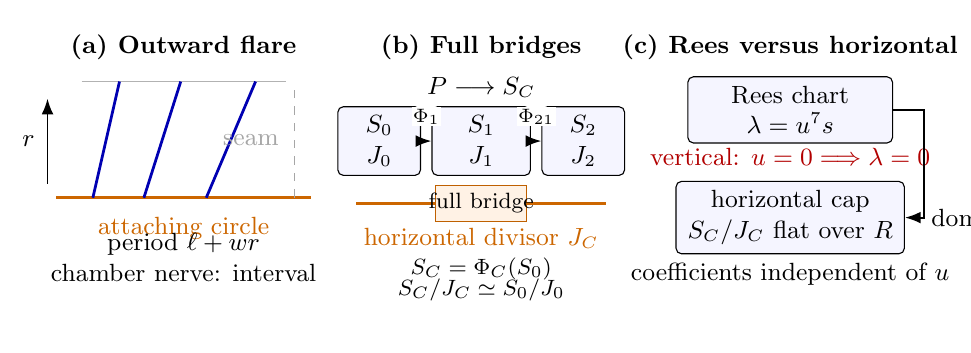
\begin{tikzpicture}[
  x=0.72cm,y=0.72cm,
  every node/.style={font=\small},
  box/.style={draw,rounded corners=2pt,fill=blue!4,minimum width=1.25cm,
    minimum height=.75cm,align=center},
  arr/.style={-{Latex[length=2mm]},line width=.7pt},
  wall/.style={line width=1pt,blue!70!black},
  boundary/.style={line width=1.1pt,orange!80!black}]
  \path[use as bounding box] (-0.5,-2.25) rectangle (15.65,3.0);

  % Panel a: developed affine flare.
  \begin{scope}[shift={(0,0)}]
    \node[font=\small\bfseries] at (2.25,2.65) {(a) Outward flare};
    \draw[boundary] (0,0) -- (4.5,0)
      node[midway,below=3pt] {attaching circle};
    \draw[gray!60] (0.45,2.05) -- (4.05,2.05);
    \draw[wall] (0.65,0) -- (1.12,2.05);
    \draw[wall] (1.55,0) -- (2.20,2.05);
    \draw[wall] (2.65,0) -- (3.52,2.05);
    \draw[dashed,gray!70] (4.2,0) -- (4.2,2.05)
      node[midway,left=2pt] {seam};
    \draw[arr] (-0.15,.25) -- (-0.15,1.75)
      node[midway,left=1pt] {$r$};
    \node[align=center] at (2.25,-1.05)
      {period $\ell+wr$\\chamber nerve: interval};
  \end{scope}

  % Panel b: transported monoid charts and full bridges.
  \begin{scope}[shift={(5.25,0)}]
    \node[font=\small\bfseries] at (2.25,2.65) {(b) Full bridges};
    \node[box,minimum width=1.05cm] (s0) at (.45,1.0) {$S_0$\\$J_0$};
    \node[box] (s1) at (2.25,1.0) {$S_1$\\$J_1$};
    \node[box,minimum width=1.05cm] (s2) at (4.05,1.0) {$S_2$\\$J_2$};
    \draw[arr] (s0.east) --
      node[above=5pt,font=\scriptsize,fill=white,inner sep=.5pt] {$\Phi_1$}
      (s1.west);
    \draw[arr] (s1.east) --
      node[above=5pt,font=\scriptsize,fill=white,inner sep=.5pt] {$\Phi_{21}$}
      (s2.west);
    \node at (2.25,1.95) {$P\longrightarrow S_C$};
    \draw[boundary] (0.05,-.10) -- (4.45,-.10);
    \draw[fill=orange!10,draw=orange!75!black] (1.45,-.42) rectangle (3.05,.22);
    \node[font=\footnotesize] at (2.25,-.10) {full bridge};
    \node[orange!80!black] at (2.25,-.72) {horizontal divisor $J_C$};
    \node[font=\footnotesize] at (2.25,-1.25)
      {$S_C=\Phi_C(S_0)$};
    \node[font=\footnotesize] at (2.25,-1.62)
      {$S_C/J_C\simeq S_0/J_0$};
  \end{scope}

  % Panel c: Rees domination versus horizontal flatness.
  \begin{scope}[shift={(10.65,0)}]
    \node[font=\small\bfseries] at (2.3,2.65) {(c) Rees versus horizontal};
    \node[box,minimum width=2.6cm] (rees) at (2.3,1.55)
      {Rees chart\\$\lambda=u^7s$};
    \node[red!70!black,fill=white,inner sep=1pt] at (2.3,.72)
      {vertical: $u=0\Longrightarrow\lambda=0$};
    \node[box,minimum width=2.9cm] (hor) at (2.3,-.35)
      {horizontal cap\\$S_C/J_C$ flat over $R$};
    \draw[arr] (rees.east) -| ++(.55,0) |- node[right=2pt,pos=.72]
      {dominates} (hor.east);
    \node[align=center] at (2.3,-1.35)
      {coefficients independent of $u$};
  \end{scope}
\end{tikzpicture}

\end{adjustbox}
\caption{A logarithmic cap.  Wall rays on the outward flare give a linear
chamber order.  Each chamber carries the transported monoid chart
$P\to S_C$, and adjacent charts are identified across a full bridge
containing the horizontal boundary.  The Rees relation controls pole order
but does not define that boundary.}
\label{fig:log-cap}
\end{figure}

There are three distinct restrictions of a finite cap.  Removing its
asymptotic divisor gives the punctured corrected mapping torus.  Reducing the
coefficient ring modulo its deformation ideal gives the toric/Kummer
scattering-special fiber.  Restricting to the asymptotic divisor gives
$\Spf(S_C/J_C)$, which remains flat over the entire coefficient ring by
\eqref{eq:horizontal-flatness}.  No coefficient variable is identified with
a spatial boundary uniformizer.

\subsection{The compactification theorem}

Truncate each flare at an integral level.  The extension of the polarization
has positive kink seven, and the product subdivision gives locally convex
boundary.  The original focus points have become peripheral end loops; their
primitive monodromies remain as holonomy rather than codimension-two
singularities of the truncation.  The finite tropical spaces are therefore
positive, locally rigid, and pre-polarized in the sense used in
\cite{carletal2024}.

\begin{theorem}[Separated fs logarithmic compactification]
\label{thm:regular-compactification}
The finite caps of Theorem~\ref{thm:finite-log-cap}, including the focus
charts \eqref{eq:focus-monoid}, form an inverse system indexed by finite root
subtrees, finite labelled coefficient systems closed under the dependencies
of Appendix~\ref{app:gkt-completion}, and deformation orders.
Each stage is separated and fs logarithmic, and its six horizontal boundary
divisors are flat over its finite Artin coefficient ring.  Its affine base
has flare widths $4,16,1,1,1,1$ and a positive integral polarization.  Its
punctured restriction carries the original annular Jacobi wall structure,
with all root, sector, exponent, and volume-line holonomies unchanged.

The inverse limit and chamber-groupoid quotient give a logarithmic
compactification in the adic proalgebraic pro-Kummer category.  No
regularity or log-regularity assertion is made, and the limit is not claimed
to be an algebraic stack of finite type.
\end{theorem}

\begin{proof}
Proposition~\ref{prop:outward-flares} supplies the affine ends and their
proper convex exhaustion.  Proposition~\ref{prop:exit-separation} supplies a
support-free seam and linearly ordered chamber cover, so every end satisfies
Theorem~\ref{thm:finite-log-cap}.  Tensoring the Kummer monoid charts
\eqref{eq:focus-monoid} with the cap monoids extends the root data.
Lemma~\ref{lem:focus-root-chart} gives fs charts and coefficient-flat
boundary at these four ends; root stacks commute with the base change.
Proposition~\ref{prop:Jacobi-transport}
then extends the volume line and its bracket.

The full bridges introduce neither doubled boundary points nor new joints.
All new charts restrict to the original ones before the exits, so
contractible consistency and every framed annular product remain unchanged.
Monic root equations and \eqref{eq:horizontal-flatness} give flatness at
each stage.  Root construction, ordered wall products, and bridge maps commute
with every finite restriction.  Passing to the compatible inverse system and
then to the groupoid quotient proves the theorem.
\end{proof}

The special fiber in this theorem is the toric/Kummer cap of the annular
model.  It is not identified with the central fiber of the original
disk-shaped quartic degeneration.  This distinction is topological as well
as categorical, and the topological half of it is an obstruction.

\begin{proposition}[No ordinary CPS recovery]
\label{prop:no-CPS-degeneration}
Neither the annular cover $\overline\Acal$ nor its noncompact
Legendre-dual cylindrical form is the dual intersection complex of a
distinguished toric degeneration of del Pezzo surfaces with simple
singularities, proper generic fiber, and smooth anticanonical divisor.
\end{proposition}

\begin{proof}
For such a degeneration the dual intersection complex is homeomorphic to
$\RR^2$ \cite[Prop.~7.13]{carletal2024}, so its first cohomology vanishes.
An annulus and an open cylinder both have $H^1(-,\Bbbk)\simeq\Bbbk$.
\end{proof}

The conclusion is limited to that class of degenerations.  It does not
exclude logarithmic or orbifold degenerations, non-proper models, a boundary
of different topology, or a comparison which agrees only on part of the
sector grading.  It does exclude reading the annulus as an unnoticed
substitute for the ordinary Carl--Pumperla--Siebert affine base.

\subsection{A regular dominating presentation}

The finite stages of Theorem~\ref{thm:regular-compactification} are not
themselves log regular in general.  This failure comes from the transported
root divisors, not from the asymptotic boundary.

\begin{proposition}[A multiple-root obstruction]
\label{prop:root-stage-nonregular}
There is a finite root-stack presentation whose atlas is singular and not log regular.
More precisely, three divisors in the orbit \eqref{eq:root-tower} meet with
distinct tangent directions at one point of the two-dimensional torus.
\end{proposition}

\begin{proof}
Write $f_A=1+x_A$ and
\[
 F_n=1+f_A^{4n}x_B.
\]
At $p=(x_A,x_B)=(-2,-1)$ one has $f_A(p)=-1$ and $F_n(p)=0$ for every
$n$.  For $n=0,1,2$ the gradients are
\[
 \nabla F_0(p)=(0,1),\qquad
 \nabla F_1(p)=(4,1),\qquad
 \nabla F_2(p)=(8,1),
\]
so the three reduced divisors are smooth and pairwise transverse at $p$.
The simultaneous root atlas has equations
\[
 r_i^2=F_i,\qquad 0\leq i\leq2.
\]
It is finite over a surface.  At the point above $p$ with all $r_i=0$, its
three-by-five Jacobian has rank two, so its tangent space has dimension
three.  The atlas is therefore singular.  If the three root divisors are put
in the log structure, the log ideal cuts out the closed point but the sharp
characteristic group has rank three.  Kato's dimension equality would read
$2=0+3$, so the chart is not log regular.  Such a finite stage occurs by
taking a rooted subtree containing the paths which give $F_0,F_1,F_2$.
\end{proof}

Regularity is recovered by a modification of the finite presentations.  The
distinction is useful: it keeps the minimal root object of
Theorem~\ref{thm:regular-compactification}, while providing a toroidal model
when regular geometry is required.

\begin{theorem}[Regular dominating presentation]
\label{thm:regular-presentation}
For every finite stage $\Xfrak_{T,\Wcal,N}$ of
Theorem~\ref{thm:regular-compactification}, over its Artin coefficient ring
$R=R_{\Wcal,N}$, there is a cofiltered system of proper morphisms
\[
 \Xfrak^{\mathrm{reg}}_{\lambda}
 \longrightarrow \Xfrak_{T,\Wcal,N}
\]
with the following properties.

\begin{enumerate}
\item Each morphism is an isomorphism away from the spatial boundary and the
transported slab-zero divisors.

\item Each $\Xfrak^{\mathrm{reg}}_{\lambda}$ is a separated logarithmic
Deligne--Mumford stack, log smooth over $(\Spec R,0)$, and has a smooth atlas
over $R$.  Every geometric fiber has a regular atlas and is log regular.

\item Its total logarithmic boundary is simple normal crossings on an
etale atlas.  In particular, the six asymptotic divisors remain flat over
$R$.

\item All finite root phases, the volume line, the Jacobi bracket,
the wall maps, and the corrected peripheral transports pull back.  Full
bridges and seams lift to strict logarithmic isomorphisms.

\item Common refinements are compatible with enlargement of the root tree,
restriction of $\Wcal$, and reduction of $N$.  Their inverse system carries
the chamber-groupoid action and gives a regularized adic pro-Kummer
compactification dominating that of
Theorem~\ref{thm:regular-compactification}.
\end{enumerate}

For a fixed resolved boundary, its component-root maps are Kummer log
etale.  A transition which introduces a previously absent root divisor is
not asserted to be Kummer log etale.
\end{theorem}

\begin{proof}
Fix the finite stage and form the reduced union $\Delta_T$ of its toric
boundary and its finitely many transported root divisors.  The root
radicands have deformation degree zero, so this pair is defined over
$\Bbbk$ and then base-changed to $R$.  First apply functorial logarithmic
resolution in characteristic zero to the root-free toroidal chart:
\[
 \rho:Z_T^{\mathrm{sm}}\longrightarrow Z_T.
\]
This is an isomorphism off $\Delta_T$, and $Z_T^{\mathrm{sm}}$ is a smooth
toroidal orbifold.  On it, functorially principalize the product of the
pulled-back radicand ideals, obtaining
\[
 \pi:Y_T\longrightarrow Z_T^{\mathrm{sm}},
 \qquad \widetilde\pi=\rho\circ\pi:Y_T\longrightarrow Z_T.
\]
Then $Y_T$ is smooth and the reduced total transform $D_T$ is simple normal
crossings \cite{abramovicheta2020principalization}.  Both steps are
functorial for toroidal isomorphisms, hence for the chamber maps, full
bridges, finite diagonal actions, and seams.

Etale locally, let $x_1,\ldots,x_s$ cut out the components of $D_T$.  For
every radicand $f_\alpha$ of degree $d_\alpha\in\{2,4\}$, principalization
gives
\[
 \widetilde\pi^*f_\alpha
 =u_\alpha\prod_{j=1}^s x_j^{a_{\alpha j}},
 \qquad u_\alpha\in\Ocal_{Y_T}^{\times}.
\]
Take the fourth root stack of every component, writing $x_j=y_j^4$, and
etale locally retain all solutions of
$\eta_\alpha^{d_\alpha}=u_\alpha$.  Then
\begin{equation}\label{eq:resolved-root-formula}
 g_\alpha=\eta_\alpha
 \prod_{j=1}^s y_j^{4a_{\alpha j}/d_\alpha}
 \qquad\text{satisfies}\qquad
 g_\alpha^{d_\alpha}=\widetilde\pi^*f_\alpha.
\end{equation}
All exponents are integral.  Thus the component-root stack maps to the
original root-stack presentation and retains its full root-choice orbit.  At a $B$ cusp,
$f_B=h^2$, formula \eqref{eq:resolved-root-formula} reads
$h=y^4$ and $g=\eta y^2$.  The ambient $\mu_4$ action exchanges the two
normalized quadratic branches, while the effective class on either branch
has order two, as in \eqref{eq:cusp-roots}.

Before the finite diagonal quotient, an etale local atlas is smooth over
$R$ with boundary $y_1\cdots y_s=0$.  Its chart is
$0\to\NN^s$, so Kato's chart criterion proves log smoothness
\cite{kato1989log}.  Finite diagonal groups are etale in characteristic zero;
their quotients are therefore log-smooth Deligne--Mumford stacks.  Geometric
fibers have regular atlases with simple-normal-crossings boundary and hence
are log regular.  The fourth-root map
$\NN^s\to\frac14\NN^s$ is Kummer log etale.  Smoothness over $R$ and the
normal-crossings description also give flatness of the asymptotic divisors.

The resolution--principalization composite is an isomorphism on the punctured
transport locus, so all wall, line, and theta data pull back unchanged.  Given
two finite regularizations, pass to the rooted union of their stages, take the
closure of their common graph, and apply the same
resolution--principalization procedure.  This gives a regular model
dominating both.  The resulting index category is cofiltered.  Path
concatenation reindexes it, while functoriality under isomorphisms lifts the
groupoid action.  This proves the pro-system assertion.  Finally, adding a
new branch divisor raises the characteristic rank at its generic point, so
such an enlargement map need not be Kummer; this explains the qualifier in
the statement.
\end{proof}

\section{GKT factors inside annular scattering}
\label{sec:gkt-decoration}

The consistent wall structure is determined by the two singleton factors and
the requirement that the path-ordered product about every joint be the
identity.  A
GKT endpoint operation has a different origin: it is the transition between
two systems of open invariants defined by canonical multisections.  The two
constructions use the same Hamiltonian Lie algebra after the $\kappa$-shift,
but their coefficients need not agree.  This section identifies their exact
relation.

\subsection{Labelled critical algebras}

Let $Q=Q_{\GKT}=(\ZZ/4)^2$ be the ordered residue group of
\eqref{eq:GKT-residue-group}.  An object $\mathcal I=(I,\tau)$ consists of a
finite set and a twist map $\tau:I\to Q$; morphisms are twist-preserving
bijections.  Put
\begin{equation}\label{eq:labelled-ring}
 A_{\mathcal I}
 =\QQ[\{u_{i,d}:i\in I, d\geq0\}]
  /\langle u_{i,d}u_{i,d'}:i\in I\rangle.
\end{equation}
Thus two variables belonging to the same marking label have zero product.

Write $\tau(i)=(a_i,b_i)$ with representatives in $\{0,1,2,3\}^2$.  The
quartic GKT critical Lie algebra is spanned over $A_{\mathcal I}$ by
$u_{J,\mathbf d}X_k$, where $J\subset I$ is nonempty,
$u_{J,\mathbf d}=\prod_{i\in J}u_{i,d_i}$, and
\begin{equation}\label{eq:critical-conditions}
 k\equiv\sum_{i\in J}\tau(i)\pmod4,
 \qquad
 k_1+k_2=\sum_{i\in J}\bigl(a_i+b_i+4(d_i-1)\bigr).
\end{equation}
The vector field is
\begin{equation}\label{eq:GKT-generator}
 X_k=x^{k_1}y^{k_2}
 \bigl((k_2+1)x\partial_x-(k_1+1)y\partial_y\bigr).
\end{equation}
The marginal generator $X_{0,0}=x\partial_x-y\partial_y$ is adjoined when
it occurs.

\begin{theorem}[Labelled critical-algebra embedding]
\label{thm:critical-embedding}
For every $\mathcal I$, the assignment
\begin{equation}\label{eq:critical-embedding}
 \jmath_{\mathcal I}:
 u_{J,\mathbf d}X_k
 \longmapsto
 u_{J,\mathbf d}X_{k+\kappa}^{\kappa}
\end{equation}
is a natural coefficient-preserving injective Lie map from the GKT critical
algebra to the Jacobi wall algebra in the distinguished root chamber.  It sends
$X_{0,0}$ to $X_\kappa^\kappa$.  Jacobi transport carries its image to a
strictly path-natural local system on the ordered-residue cover.  The
construction commutes with relabelling, finite restriction,
and deformation truncation.
\end{theorem}

\begin{proof}
In GKT notation,
\[
 [X_k,X_\ell]
 =-\det(k+\kappa,\ell+\kappa)X_{k+\ell}.
\]
Equation~\eqref{eq:shifted-bracket} gives the same formula after applying
\eqref{eq:critical-embedding}.  If two coefficient monomials share a label,
their product vanishes in \eqref{eq:labelled-ring}; if their supports are
disjoint, both conditions in \eqref{eq:critical-conditions} add.  Hence the
assignment is a Lie map, and it is injective on the displayed monomial
basis.  The marginal bracket is preserved because
\[
 [X_{0,0},X_{a,b}]=(a-b)X_{a,b}
 =-\det(\kappa,(a,b)+\kappa)X_{a,b}.
\]
Jacobi path transport is a Lie isomorphism by
Proposition~\ref{prop:Jacobi-transport}.  On the ordered-residue cover the
$Q$-grading is constant; affine transport moves the Hamiltonian exponent and
the $\kappa$-shift together.  The remaining naturality statements are
immediate from the labelled formula.
\end{proof}

In a finite nilpotent quotient, exponential integrates
\eqref{eq:critical-embedding} to an injective group homomorphism.  The GKT
jump theorem identifies an isolated critical zero of a canonical homotopy
with the exponential of its critical-graph generator, while the
boundary-ray theorem of \cite{wuebben2026boundary} gives its unique
increasing-slope factorization, giving the following comparison.

\begin{proposition}[Finite endpoint operations]
\label{prop:endpoint-operations}
Every finite GKT endpoint transition maps to a framed Jacobi automorphism,
and its increasing-slope factors map factor by factor to the shifted rays
$\RR_{\geq0}(k+\kappa)$.  The image depends only on the realizable endpoints,
not on the chosen canonical homotopy.  It is natural under labelled
restriction and path transport.
\end{proposition}

\begin{proof}
Exponentiation and Baker--Campbell--Hausdorff are finite in the chosen
quotient and are functorial for the map of Theorem
\ref{thm:critical-embedding}.  GKT prove that their finite action on
realizable chamber indices is faithful and transitive
\cite[Thm.~4.27 and Cor.~5.14]{grossetal2022open}.  This alone would not
give uniqueness of a transition element.  The enlarged-torsor statement in
Theorem~\ref{thm:companion}, which includes the marginal generator, proves
that the enlarged action is free and transitive.  Its freeness makes
the element carrying one endpoint to the other unique.  The slope assertion
follows because $k$ maps to shifted exponent $k+\kappa$.
\end{proof}

Appendix~\ref{app:gkt-completion} strengthens this formal statement: the
finite endpoint homotopies can be chosen compatibly as the labelled system
grows.  Thus every GKT factor distinguished below has an actual finite
multisection realization.

The ordered-residue cover does not identify annular transport with standard
retwisting of one fixed polynomial critical algebra.  Indeed, the peripheral
residue action completes the singleton twists into
\[
 \{(1,0),(2,3),(3,2),(0,1)\}.
\]
Two distinct labels of twist $(1,0)$ and descendent degree one have a joint
critical block of rank one, with exponent $(2,0)$.  Retwisting both by the
matrix $P_{\mathrm{res}}$ of \eqref{eq:residue-matrix} produces three exponents
$(0,10),(4,6),(8,2)$.  Hence no coefficient-preserving linearization can
fix labels and descendent degrees while retwisting every marking by $P_{\mathrm{res}}$.
Annular transport instead moves the exponent and volume frame and
may produce root-valued Laurent expressions in the target chart.

\subsection{Enumerative and residual factors}

Take two distinct labels with
\[
 t_1=u_{i,1},\quad\tau(i)=(1,0),
 \qquad
 t_2=u_{j,1},\quad\tau(j)=(0,1),
\]
and work modulo $(t_1^2,t_2^2)$.  The two extreme GKT potentials are
\begin{equation}\label{eq:mixed-potentials}
\begin{aligned}
 W^{\min}
 &=x^4+y^4-4t_1xy^4-2t_2y^5+12t_1t_2xy^5,\\
 W^{\max}
 &=x^4+y^4-2t_1x^5-4t_2x^4y+12t_1t_2x^5y.
\end{aligned}
\end{equation}
Their increasing-slope endpoint transition is
\begin{equation}\label{eq:mixed-GKT-transition}
 \exp\!\left(-\frac12t_2X_{0,1}\right)
 \exp\!\left(\frac14t_1t_2X_{1,1}\right)
 \exp\!\left(-\frac12t_1X_{1,0}\right).
\end{equation}
By contrast, the inverse commutator of the two singleton walls has exact
mixed factor
\begin{equation}\label{eq:mixed-total-factor}
 T=\exp\!\left(\frac34t_1t_2X_{1,1}\right).
\end{equation}
Define
\begin{equation}\label{eq:mixed-decoration}
 G_{\mathrm{mix}}=\exp\!\left(\frac14t_1t_2X_{1,1}\right),
 \qquad
 R_{\mathrm{mix}}=\exp\!\left(\frac12t_1t_2X_{1,1}\right).
\end{equation}

\begin{proposition}[First GKT--residual factorization]
\label{prop:first-decoration}
The three factors lie in one abelian shifted-ray group and
\begin{equation}\label{eq:three-quarter-split}
 T=G_{\mathrm{mix}}R_{\mathrm{mix}},
 \qquad \frac34=\frac14+\frac12.
\end{equation}
The first factor on the right is the unique mixed GKT endpoint factor; the
second is the unique residual factor.  Replacing the total wall by the GKT
factor leaves contractible-loop holonomy $R_{\mathrm{mix}}^{\pm1}$.
\end{proposition}

\begin{proof}
The balanced two-label profiles are $(1,5)$ and $(5,1)$.  The GKT chamber
equations give endpoint coefficient $-12$ on each extreme.  After applying
the first singleton factor, the remaining difference in the coefficient of
$xy^5$ is two.  Since
\[
 X_{1,1}(x^4+y^4)=8x^5y-8xy^5,
\]
the mixed endpoint generator has coefficient $2/8=1/4$, proving
\eqref{eq:mixed-GKT-transition}.  Equation~\eqref{eq:first-bracket} gives the
scattering coefficient $3/4$.  The square-zero mixed ray is central, so
subtraction of logarithms gives the residual coefficient $1/2$ exactly.
The total factor is the one which cancels the joint product.
\end{proof}

There is no group projection which fixes the two incoming factors and sends
$T$ to $G_{\mathrm{mix}}$: a homomorphism fixing the inputs fixes their commutator.
Nor can a rank-one character remove $R_{\mathrm{mix}}$, since a character is trivial on the
commutator subgroup.  The GKT factor is therefore a distinguished subfactor
of the total wall, not a quotient wall of a second consistent diagram.

\subsection{All-order factorization}

Let $\mathcal I$ be a finite set of distinct descendent-one labels, each of
twist $\alpha=(1,0)$ or $\beta=(0,1)$, in the square-zero labelled ring.
For $\varnothing\ne J\subseteq\mathcal I$ put
\[
 p_J=|J_\alpha|,
 \qquad q_J=|J_\beta|,
\]
and write
$p_J=r_J+4\ell_J$, $q_J=s_J+4m_J$ with
$0\leq r_J,s_J\leq3$.  The balanced profiles and critical exponents in the
full-support GKT block are
\begin{align}
 b_{J,h}
 &=(r_J+4h,s_J+4(\ell_J+m_J+1-h)),
 &&0\leq h\leq\ell_J+m_J+1,\label{eq:balanced-profiles}\\
 k_{J,h}
 &=(r_J+4h,s_J+4(\ell_J+m_J-h)),
 &&0\leq h\leq\ell_J+m_J.\label{eq:critical-profiles}
\end{align}
Write
\[
 b_J^{\min}=b_{J,0},
 \qquad
 b_J^{\max}=b_{J,\ell_J+m_J+1},
\]
and let $\nu_J^\epsilon$ be the full-support endpoint invariant in the
chamber $\epsilon\in\{\min,\max\}$.  For any exponent $(u,v)$ in this
residue class, set
\begin{equation}\label{eq:quartic-Gamma-weight}
 w_J(u,v)=
 \frac{\Gamma((u+1)/4)\Gamma((v+1)/4)}
      {\Gamma((r_J+1)/4)\Gamma((s_J+1)/4)}.
\end{equation}
This is the quartic Gamma weight in the GKT chamber equation; it is nonzero
for all balanced profiles occurring here.

Let
\begin{equation}\label{eq:GKT-logarithm-J}
 E_J=t_J\sum_hg_{J,h}X_{k_{J,h}}
\end{equation}
be the unique slope-ordered GKT endpoint logarithm.  If $a_{p,q}$ is the
coefficient of $E_{p,q}$ in the unlabelled singleton scattering
factorization, set $a_{p,0}=a_{0,q}=0$ for $p,q>0$ and define the
full-support scattering logarithm
\begin{equation}\label{eq:scattering-logarithm-J}
 S_J=p_J!q_J!a_{p_J,q_J}t_JX_{p_J,q_J}.
\end{equation}
For a shifted ray $\mathfrak r$, let $E_{\mathfrak r}$ and
$S_{\mathfrak r}$ be the sums of the corresponding terms and put
\begin{equation}\label{eq:residual-ray}
 R_{\mathfrak r}=S_{\mathfrak r}-E_{\mathfrak r}.
\end{equation}

\begin{theorem}[Canonical all-order GKT factorization]
\label{thm:all-order-decoration}
The endpoint recursions determine every coefficient in
\eqref{eq:GKT-logarithm-J} canonically, and
\begin{equation}\label{eq:decorated-word}
 \overrightarrow{\prod_{\mathfrak r}}\exp(S_{\mathfrak r})
 =\overrightarrow{\prod_{\mathfrak r}}
  \bigl(\exp(E_{\mathfrak r})\exp(R_{\mathfrak r})\bigr).
\end{equation}
The equality is raywise; no factor is commuted past a factor on another
slope.  It is natural under relabelling, deletion of labels, restriction of
finite labelled systems closed under the dependencies of
Appendix~\ref{app:gkt-completion}, reduction of deformation order, and framed
Jacobi transport.  It adds no new geometric support to the annular diagram.
\end{theorem}

\begin{proof}
The GKT dimension formula gives
\eqref{eq:balanced-profiles}--\eqref{eq:critical-profiles}.  For an endpoint
$\epsilon\in\{\min,\max\}$, the full-support invariant is determined by the
partition recursion
\begin{equation}\label{eq:endpoint-recursion}
 w_J(b_J^\epsilon)\nu_J^\epsilon
 +\sum_{\substack{\pi\in\operatorname{Part}(J)\\|\pi|\geq2}}
 w_J\!\left(\sum_{C\in\pi}b_C^\epsilon\right)
 \prod_{C\in\pi}\nu_C^\epsilon
 =\begin{cases}-1,&|J|=1,\\0,&|J|\geq2.
 \end{cases}
\end{equation}
The coefficient of $\nu_J^\epsilon$ is a nonzero Gamma weight, so induction
on $|J|$ determines the endpoints.  The critical generators form the
weighted incidence matrix of the path of balanced profiles.  Indeed,
\begin{equation}\label{eq:critical-incidence}
 X_{u,v}(x^4+y^4)
 =4(v+1)x^{u+4}y^v-4(u+1)x^uy^{v+4}.
\end{equation}
For $(u,v)=k_{J,h}$ the two monomials in
\eqref{eq:critical-incidence} are precisely the adjacent vertices
$b_{J,h+1}$ and $b_{J,h}$.  The resulting path incidence matrix has full
column rank, and its one left-kernel relation is the chamber equation.
Hence the coefficients $g_{J,h}$ exist and are unique.

For the scattering term, substitute
\[
 t_\alpha=\sum_{\tau(i)=\alpha}t_i,
 \qquad t_\beta=\sum_{\tau(i)=\beta}t_i
\]
in the unlabelled factorization.  The coefficient of $t_J$ in
$t_\alpha^{p_J}t_\beta^{q_J}$ is $p_J!q_J!$, which gives
\eqref{eq:scattering-logarithm-J}.  Both constructions are triangular in
proper subsets, proving naturality under restriction.  Generators on one
shifted ray commute, so \eqref{eq:residual-ray} exponentiates and yields
\eqref{eq:decorated-word}.  A nonzero $E_{\mathfrak r}$ with
$S_{\mathfrak r}=0$ is recorded as the identity pair
$\exp(E_{\mathfrak r})\exp(-E_{\mathfrak r})$, not as a geometric wall.
\end{proof}

\subsection{Compatible geometric realization}

The preceding factorization has a geometric realization.  The relative
extension arguments in Appendix~\ref{app:gkt-completion} give the following
geometric realization theorem.

For the theorem, an \emph{exact GKT datum} is a graded open $(4,4)$-graph
together with its descendent vector.  A \emph{finite partial system} records
a finite twist-labelled set, a finite set of labelled monomials closed under
divisors, and finitely many exact data closed under the connected-component
and boundary dependencies of the GKT assembling relation.  The precise
definition is given in Appendix~\ref{app:gkt-completion}.

\begin{theorem}[Compatible completed GKT realization]
\label{thm:compatible-GKT-realization}
There are nested finite partial systems
$\mathbb D_1\subset\mathbb D_2\subset\cdots$ exhausting all exact GKT data,
compatible canonical families realizing the two extremal chamber indices,
and a componentwise smooth GKT homotopy between them such that:
\begin{enumerate}
\item the countably many ray factors occur in pairwise disjoint open time
intervals, ordered by increasing slope;
\item each fixed component is nonconstant on only finitely many such
intervals and has constant endpoint collars;
\item every finite divisor-closed quotient has precisely its prescribed
finite collection of nonzero ray jumps; and
\item the finite restrictions form an inverse limit in the category of
sets.
\end{enumerate}
Simplicity is asserted for the finite elementary homotopies, not for one
global assignment of jump times to all label subsets.
\end{theorem}

Thus every GKT factor in Theorem~\ref{thm:all-order-decoration} is the image
of an actual finite restriction of a compatible homotopy.  The residual
factors are not enumerative jumps; they remain comparison automorphisms.

\subsection{Residual coherence}

The residual factors can be retained coherently in multiplication.  Fix a
finite labelled system and two framed input paths.  Let $U_i$ be the
total consistent transport, $V_i$ its GKT subword, and
$Q_i=U_iV_i^{-1}$ the residual transport.  In a finite nilpotent quotient
define the midpoint
\begin{equation}\label{eq:residual-midpoint}
 H=Q_1(Q_1^{-1}Q_2)^{1/2},
 \qquad C_i=HQ_i^{-1}.
\end{equation}
Rational powers are the finite polynomials $g^c=\exp(c\log g)$.

\begin{lemma}\label{prop:residual-midpoint}
The midpoint is symmetric in $Q_1,Q_2$ and
\begin{equation}\label{eq:corrected-product}
 C_iU_i=HV_i,
 \qquad
 \mu(C_1U_1f_1,C_2U_2f_2)=H\mu(V_1f_1,V_2f_2).
\end{equation}
It is natural under finite restriction and bi-equivariant under common
terminal total and GKT transports.
\end{lemma}

\begin{proof}
With $A=Q_1^{-1}Q_2$,
$Q_2(Q_2^{-1}Q_1)^{1/2}=Q_1A(A^{-1})^{1/2}=Q_1A^{1/2}$, proving symmetry.
The first identity in \eqref{eq:corrected-product} is immediate; the second
uses that $H$ is an algebra automorphism.  Conjugation-equivariance of
rational powers gives the claimed bi-equivariance.
\end{proof}

For positive degrees $r,s$, set
\begin{equation}\label{eq:weighted-interpolation}
 M_{r,s}(P,Q)=P(P^{-1}Q)^{s/(r+s)}.
\end{equation}
For a rooted binary product tree, recursively define a residual interpolant,
with weights equal to the sums of the leaf degrees.

\begin{proposition}[Degree-weighted coherence]
\label{thm:residual-coherence}
If $H_\tau$ is the interpolant associated with a product tree $\tau$, its
corrected product is
\[
 \mathsf P_\tau=H_\tau\prod_iV_if_i.
\]
For two trees $\tau,\sigma$, the automorphism
$\mathcal A_{\tau\leftarrow\sigma}=H_\tau H_\sigma^{-1}$ carries one
product to the other and satisfies
\[
 \mathcal A_{\tau\leftarrow\sigma}
 \mathcal A_{\sigma\leftarrow\rho}
 =\mathcal A_{\tau\leftarrow\rho}.
\]
All associahedral coherence identities therefore hold.  For three
equal-degree residuals $e^x,e^y,e^z$ in the free labelled square-zero group,
\begin{equation}\label{eq:first-associator}
 \log\mathcal A_{L\leftarrow R}=\frac1{72}[[x,z],y].
\end{equation}
The comparison is coherent but not generally strict monoidal.
\end{proposition}

\begin{proof}
At an internal vertex, the corrections carry both child products to the
same interpolant $H_\tau$.  Since this interpolant is an algebra automorphism, induction
gives the displayed form of $\mathsf P_\tau$.  Ratios of interpolants carry one
tree product to another, and cancellation proves the cocycle identity.
The weighted interpolation is symmetric under exchange of the two weighted
children and is equivariant under the left--right bitorsor action.
Baker--Campbell--Hausdorff expansion for three equal weights gives the common
linear term $(x+y+z)/3$, no quadratic difference, and cubic difference
\[
 \frac1{72}(xzy-zxy-yxz+yzx)
 =\frac1{72}[[x,z],y],
\]
which is \eqref{eq:first-associator}.  By comparison, unweighted iteration
assigns leaf weights $(1/4,1/4,1/2)$ and $(1/2,1/4,1/4)$ in the two
parenthesizations already in the abelian quotient.
\end{proof}

Changes of framed input paths act on the individual legs as well as on the
output interpolant.  The precise naturality statement is the following.

Let $\Gamma=(\gamma_i)$ and $\Gamma'=(\gamma_i')$ be two tuples of framed
input paths with the same endpoints.  For a fixed product tree,
write $V_i^\Gamma,V_i^{\Gamma'}$ for the corresponding GKT transports and
$H_\Gamma,H_{\Gamma'}$ for their residual interpolants.  Put
\begin{equation}\label{eq:corridor-maps}
 W_i^{\Gamma'\leftarrow\Gamma}
   =V_i^{\Gamma'}(V_i^\Gamma)^{-1},
 \qquad
 B^{\Gamma'\leftarrow\Gamma}
   =H_{\Gamma'}H_\Gamma^{-1}.
\end{equation}

\begin{lemma}[Change of framed paths]
\label{prop:corridor-groupoid}
For $a_i=V_i^\Gamma f_i$ one has the commutative comparison square
\begin{equation}\label{eq:corridor-square}
 H_{\Gamma'}\prod_iV_i^{\Gamma'}f_i
 =B^{\Gamma'\leftarrow\Gamma}H_\Gamma
   \prod_i\bigl(W_i^{\Gamma'\leftarrow\Gamma}a_i\bigr).
\end{equation}
The leg maps and output maps compose under successive changes of framed paths, and
the resulting squares commute with the tree-transition cocycle of
Proposition~\ref{thm:residual-coherence}.  Thus path and tree changes form a
coherent factorization groupoid.

There is no output-only descent for arbitrary independent changes of the input paths.
In particular, if one leg changes by a nontrivial unital automorphism $W$
and another leg is fixed, no output automorphism $Z$ can satisfy
$Z(ab)=W(a)b$ for all $a,b$.
\end{lemma}

\begin{proof}
The identities
$V_i^{\Gamma'}f_i=W_i^{\Gamma'\leftarrow\Gamma}a_i$ and
$B^{\Gamma'\leftarrow\Gamma}H_\Gamma=H_{\Gamma'}$ give
\eqref{eq:corridor-square}.  For a third tuple $\Gamma''$, cancellation
gives
\[
 W_i^{\Gamma''\leftarrow\Gamma'}
 W_i^{\Gamma'\leftarrow\Gamma}
 =W_i^{\Gamma''\leftarrow\Gamma},
 \qquad
 B^{\Gamma''\leftarrow\Gamma'}
 B^{\Gamma'\leftarrow\Gamma}
 =B^{\Gamma''\leftarrow\Gamma}.
\]
Tree transitions are likewise ratios of the corresponding centers, so the
mixed squares commute by the same cancellation.  Finally, if
$Z(ab)=W(a)b$, then $b=1$ gives $Z=W$, whereas $a=1$ gives
$Z=\mathrm{id}$.  Hence an output-only comparison exists only when the leg
change is trivial.
\end{proof}

The result of this section is therefore a coherent factorization comparison.
The total factors remain the walls of the consistent diagram.  The GKT
endpoint factors are marked inside them, and the residual automorphisms are
retained as comparison data.  No equality between these wall coefficients
and commutative theta structure constants has been asserted.

\section{Transport of the primary Frobenius structure}
\label{sec:primary-frobenius}

Section~\ref{sec:gkt-decoration} compares wall-crossing groups.  A comparison
of Frobenius structures requires further data: a primitive form, oscillatory
periods, a residue pairing, and a Kodaira--Spencer basis.  This section
supplies these data on the primary slice, where every descendent variable
vanishes, starting from the primary potential of \cite{grossetal2022open}
with the primitive form $dx\wedge dy$ in the sense of
\cite[Def.~4.3]{grossetal2022open}, recalled below.  The annular geometry
enters only through the transition maps between charts; these are algebra
isomorphisms onto their images, and they preserve the Frobenius structure by
transport of structure (Proposition~\ref{thm:primary-Frobenius}).  The source
structure is calibrated in Appendix~\ref{app:primary-calibration},
independently of the annulus: the primary potential has a unique
representative $W^{\GKT}_{\mathrm{prim}}$ invariant under the exchange of the
coordinates, for which $dx\wedge dy$ is a primitive form with the nine
primary variables as flat coordinates (Lemma~\ref{lem:reflection-fixed} and
the discussion after it).
On the marginal line $W^{\GKT}_{\mathrm{prim}}$ is the flat structure of
Noumi and Yamada with primitive form normalized to $dx\wedge dy$, and its
coefficients give the first open invariants of the reflection-fixed chamber
index (Theorem~\ref{thm:marginal-calibration}).

In the \emph{source chart}, given by the fixed frame of the sheet $S_0$
(Sections~\ref{sec:affine-kummer} and~\ref{sec:jacobi-theta}), we write
$x=z_1$ and $y=z_2$.  Under the dictionary of Section~\ref{sec:jacobi-theta}
these are the coordinates of the GKT potentials in \cite{grossetal2022open}
and in Sections~\ref{sec:gkt-decoration} and~\ref{sec:positive-descendents},
not the Cox coordinates of \eqref{eq:quartic-pencil}.  Then
$dx\wedge dy=\Omega_\kappa$ by \eqref{eq:primitive-form}, and the
Hamiltonian fields $X_{a,b}=X^\kappa_{\kappa+(a,b)}$ of
Proposition~\ref{prop:shifted-bracket}, of divergence zero for
$dx\wedge dy$, are
\begin{equation}\label{eq:quartic-vector-field}
 X_{a,b}
 =x^ay^b\bigl((b+1)x\partial_x-(a+1)y\partial_y\bigr).
\end{equation}
The symmetric deformation variables of \cite[Def.~4.10]{grossetal2022open}
are $t_{a,b,d}$, $0\leq a,b\leq2$, $d\geq0$, where $(a,b)$ is a twist and $d$
is the descendent index.  The \emph{primary variables} are those with $d=0$,
and we write
$t_{a,b}=t_{a,b,0}$.  The variable $t_{a,b}$ is the parameter dual to the
monomial $x^ay^b$; the nine monomials $x^ay^b$, $0\leq a,b\leq2$, form a basis
of the Jacobian ring $\Jac(x^4+y^4)$ and correspond to the nine narrow
elements $(e^{2\pi i(a+1)/4},e^{2\pi i(b+1)/4})$ of $\mu_4\times\mu_4$,
those whose fixed locus in $\CC^2$ is the origin.  Put
\begin{equation}\label{eq:primary-base}
 A_{\mathrm{prim}}
 =\QQ[[t_{a,b}:0\leq a,b\leq2]],
 \qquad \mathfrak m_{\mathrm{prim}}=(t_{a,b}).
\end{equation}
A statement over this complete ring means a compatible system of statements
over the quotients $\QQ[t_{a,b}]/(t_{a,b}^{n_{a,b}+1})$.  For the source
potential the compatibility is part of Lemma~\ref{lem:reflection-fixed}.
The exchange of the coordinates and the degree-zero field, the case
$(a,b)=(0,0)$ of \eqref{eq:quartic-vector-field}, are
\begin{equation}\label{eq:reflection}
 \sigma(x,y,t_{a,b})=(y,x,t_{b,a}),
 \qquad
 X_{0,0}=x\partial_x-y\partial_y .
\end{equation}

The periods are taken over the good basis of
\cite[\S4.1]{grossetal2022open}: the product cycles $\Xi_{a,b}$,
$0\leq a,b\leq2$, in the relative homology
$H_2(\CC^2,\operatorname{Re}(x^4+y^4)/\hbar\ll0;\CC)$, dual to the
monomial basis in the sense that
\[
 \int_{\Xi_{a,b}}x^cy^d\,e^{(x^4+y^4)/\hbar}\,dx\wedge dy
 =\delta_{ac}\delta_{bd},
 \qquad 0\leq c,d\leq2
\]
\cite[(4.3)]{grossetal2022open}.  The same integrals for arbitrary
$c,d\geq0$, the \emph{moments}, follow by integration by parts
\cite[Lem.~4.2]{grossetal2022open}.  For a deformation $W$ of $x^4+y^4$ over
a complete local ring, the period of $(W,dx\wedge dy)$ over $\Xi_{a,b}$ is
the formal series in $\hbar$ and $\hbar^{-1}$ obtained by expanding
$\int_{\Xi_{a,b}}e^{W/\hbar}\,dx\wedge dy$ in the moments.  Following
\cite[Def.~4.3]{grossetal2022open}, $dx\wedge dy$ is a \emph{primitive form}
for $W$ if, for every $0\leq a,b\leq2$, the period over $\Xi_{a,b}$ contains
no positive power of $\hbar$ and has constant term
$\delta_{(a,b),(0,0)}$; the coefficients of $\hbar^{-1}$ in the nine periods
are then the \emph{flat coordinates}.  Thus $dx\wedge dy$ is a primitive
form with flat coordinates $t_{a,b}$ exactly when
\[
 \int_{\Xi_{a,b}}e^{W/\hbar}\,dx\wedge dy
 =\delta_{(a,b),(0,0)}+\hbar^{-1}t_{a,b}+O(\hbar^{-2}),
 \qquad 0\leq a,b\leq2,
\]
which is the form in which \cite[Cor.~4.17]{grossetal2022open} states it.
GKT formulate the definition for a form $f\,dx\wedge dy$ and present it as
a simplified version of Saito's theory of primitive forms; only $f=1$ occurs
here.

\subsection{The source Frobenius algebra}
\label{subsec:source-Frobenius}

At the Fermat point the primary state space is
\begin{equation}\label{eq:Fermat-Jacobian}
 H_{4,4}=\QQ[x,y]/(x^3,y^3),
 \qquad e_{a,b}=[x^ay^b],\quad 0\leq a,b\leq2.
\end{equation}
Normalize the Grothendieck residue trace by
\begin{equation}\label{eq:residue-trace}
 \epsilon_0(f)
 =16\operatorname{Res}_0
   \frac{f\,dx\wedge dy}{(4x^3)(4y^3)}.
\end{equation}

\begin{proposition}[Residue pairing at the Fermat point]
\label{prop:classical-vertex}
The pairing $\eta_0(f,g)=\epsilon_0(fg)$ on $H_{4,4}$ is nondegenerate and
\begin{equation}\label{eq:classical-pairing}
 \eta_0(e_{a,b},e_{c,d})
 =\delta_{a+c,2}\delta_{b+d,2}.
\end{equation}
Equivalently, $\epsilon_0$ is the coefficient of the socle monomial
$e_{2,2}$, and $e_{a,b}e_{2-a,2-b}=e_{2,2}$ for $0\leq a,b\leq2$.
\end{proposition}

\begin{proof}
The residue in \eqref{eq:residue-trace} extracts the coefficient of
$x^2y^2$.  Since $e_{a,b}e_{c,d}=e_{a+c,b+d}$ when $a+c\leq2$ and $b+d\leq2$
and vanishes otherwise, this proves \eqref{eq:classical-pairing}, the socle
identity, and nondegeneracy.
\end{proof}

Over the primary base, the Jacobian algebra of the reflection-fixed primary
potential and its normalized residue trace are
\begin{equation}\label{eq:source-primary-Jacobian}
 \mathcal R_0=A_{\mathrm{prim}}[x,y]\big/
  (\partial_xW^{\GKT}_{\mathrm{prim}},
   \partial_yW^{\GKT}_{\mathrm{prim}}),
 \qquad
 \epsilon(h)=16\operatorname{Res}_0
 \frac{h\,dx\wedge dy}
 {\partial_xW^{\GKT}_{\mathrm{prim}}\,\partial_yW^{\GKT}_{\mathrm{prim}}},
\end{equation}
with residue pairing $\eta(f,g)=\epsilon(fg)$ and Kodaira--Spencer classes
$\Phi^0_{a,b}=[\partial W^{\GKT}_{\mathrm{prim}}/\partial t_{a,b}]$,
$0\leq a,b\leq2$.

\begin{lemma}[Source Frobenius algebra]
\label{lem:source-Frobenius}
The classes $\Phi^0_{a,b}$ form an $A_{\mathrm{prim}}$-basis of
$\mathcal R_0$, with $\Phi^0_{a,b}=x^ay^b+O(\mathfrak m_{\mathrm{prim}})$
and $\Phi^0_{0,0}=[1]$.  The pairing $\eta$ is nondegenerate and makes
$\mathcal R_0$ a Frobenius algebra.  Under the Kodaira--Spencer map
$\partial/\partial t_{a,b}\mapsto\Phi^0_{a,b}$, the multiplication of
$\mathcal R_0$ and $\eta$ are the product and the flat metric of the primary
Saito--Givental Frobenius manifold of $W^{\GKT}_{\mathrm{prim}}$; in
particular $\eta$ is constant in the flat coordinates $t_{a,b}$.  By
\cite[Thm.~0.3 and Rem.~0.4(2)]{grossetal2022open}, this Frobenius manifold
is the genus-zero primary closed FJRW Frobenius manifold of
$(x^4+y^4,\mu_4^2)$.
\end{lemma}

\begin{proof}
Modulo quadratic terms in the $t_{a,b}$,
$W^{\GKT}_{\mathrm{prim}}\equiv x^4+y^4+\sum t_{a,b}x^ay^b$
\cite[Def.~3.47(1) and (4.11)]{grossetal2022open}, which gives the
congruence for $\Phi^0_{a,b}$.  Over each quotient $A^{\mathrm{prim}}_I$,
where $\mathfrak m_{\mathrm{prim}}$ is nilpotent, the nine monomials $x^ay^b$
span $\mathcal R_0$ by Nakayama's lemma, since they span
$\mathcal R_0/\mathfrak m_{\mathrm{prim}}\mathcal R_0=H_{4,4}$.  The
functional $\epsilon$ vanishes on the Jacobian ideal, and the Gram matrix of
$\eta$ on these monomials reduces modulo $\mathfrak m_{\mathrm{prim}}$ to the
invertible matrix of Proposition~\ref{prop:classical-vertex}, so its
determinant is a unit.  Hence $\mathcal R_0$ is free with basis the
$x^ay^b$ and $\eta$ is nondegenerate; the $\Phi^0_{a,b}$ form a basis by
Nakayama's lemma, $\Phi^0_{0,0}=[1]$ by \eqref{eq:constant-deformation}, and
$\eta(fg,h)=\epsilon(fgh)=\eta(f,gh)$.  The flat coordinates $t_{a,b}$ of
$(W^{\GKT}_{\mathrm{prim}},dx\wedge dy)$ (the discussion after
Lemma~\ref{lem:reflection-fixed}) agree with those of Saito--Givental theory
in the good-basis description of \cite[\S2.2]{heetal2022}
\cite[Rems.~0.4(2) and~4.5]{grossetal2022open}, so the Kodaira--Spencer map
identifies the product and flat metric of Saito's Frobenius manifold
\cite{saito1983period} with the multiplication of $\mathcal R_0$ and $\eta$.
Every symmetric chamber index is enumerative
\cite[Prop.~3.46 and Cor.~5.14]{grossetal2022open}, so
\cite[Thm.~0.3 and Rem.~0.4(2)]{grossetal2022open} applies.
\end{proof}

\subsection{Transport through the annular charts}
\label{subsec:KS-classes}

Let $R$ be an Artinian local $\QQ$-algebra of labelled deformation
coefficients, base-changed to $\Bbbk$ where it meets the chart algebras
(Section~\ref{sec:introduction}).  For $W\in R[x,y]$ the Brieskorn module is
\begin{equation}\label{eq:Brieskorn-module}
 \operatorname{GM}_\hbar(W)
 =H^2\!\left(
  \Omega_{R[x,y]/R}^{\bullet}[[\hbar]],
  \hbar d+dW\wedge
 \right).
\end{equation}
For an admissible path $\mathfrak p$ (Definition~\ref{def:framed-path}), let
$P_{\mathfrak p}$ be the composite of the transition maps along it: the slab
maps \eqref{eq:local-root-ring} with the affine holonomy they carry, and the
wall automorphisms.  These are injective homomorphisms of $R$-algebras
between chart algebras, so $U_{\mathfrak p}=P_{\mathfrak p}(x)$ and
$V_{\mathfrak p}=P_{\mathfrak p}(y)$ are algebraically independent over $R$,
and $P_{\mathfrak p}$ is an isomorphism onto the image algebra
\begin{equation}\label{eq:image-algebra}
 P_{\mathfrak p}\bigl(R[x,y]\bigr)=R[U_{\mathfrak p},V_{\mathfrak p}]
\end{equation}
inside the target chart algebra.  Brieskorn modules, Jacobian algebras,
residue pairings and good-basis periods (the moment functionals of
\cite[Lem.~4.2]{grossetal2022open}) of $P_{\mathfrak p}W$ are formed over
this image algebra by the same formulas in $U_{\mathfrak p},V_{\mathfrak p}$,
not over the target chart algebra, a Laurent algebra over which the Jacobian
quotient of a transported primary potential vanishes because its
$U_{\mathfrak p}$-derivative is a unit.  The periods are
formal functionals, since the torus of the target chart does not contain the
critical point $U_{\mathfrak p}=V_{\mathfrak p}=0$.  By \eqref{eq:slab-conformal}, $dU_{\mathfrak p}\wedge
dV_{\mathfrak p}$ is the form $\Omega'_\kappa$ of the target chart times the
unit recorded by the line $\Lcal_\kappa$.

On the primary slice put
$W_{\mathfrak p}=P_{\mathfrak p}(W^{\GKT}_{\mathrm{prim}})$,
\begin{equation}\label{eq:transported-primary-Jacobian}
 \mathcal R_{\mathfrak p}
 =A_{\mathrm{prim}}[U_{\mathfrak p},V_{\mathfrak p}]\big/
  (\partial_{U_{\mathfrak p}}W_{\mathfrak p},
   \partial_{V_{\mathfrak p}}W_{\mathfrak p}),
\end{equation}
let $\eta_{\mathfrak p}$ be the residue pairing of
$(W_{\mathfrak p},dU_{\mathfrak p}\wedge dV_{\mathfrak p})$, and let
\begin{equation}\label{eq:KS-sections}
 \Phi_{a,b}^{\mathfrak p}
 =\left[\frac{\partial W_{\mathfrak p}}{\partial t_{a,b}}\right]
 \in\mathcal R_{\mathfrak p},
 \qquad 0\leq a,b\leq2,
\end{equation}
be the transported Kodaira--Spencer classes; for the trivial path these are
the $\Phi^0_{a,b}$ of Lemma~\ref{lem:source-Frobenius}.

\begin{proposition}[Transported primary Frobenius structure]
\label{thm:primary-Frobenius}
\label{prop:Brieskorn-transport}
\label{thm:primary-Saito-system}
Let $\mathfrak p$ be an admissible path.
\begin{enumerate}
\item For $W\in R[x,y]$, $P_{\mathfrak p}$ induces an isomorphism of twisted
de Rham complexes over $R[[\hbar]]$, and hence
\begin{equation}\label{eq:Brieskorn-transport}
 \operatorname{GM}_\hbar(W)
 \xrightarrow{\sim}
 \operatorname{GM}_\hbar(P_{\mathfrak p} W),
\end{equation}
carrying $[dx\wedge dy]$ to $[dU_{\mathfrak p}\wedge dV_{\mathfrak p}]$.
Modulo $\hbar$ it identifies the Jacobian algebras and the residue pairings of
$(W,dx\wedge dy)$ and $(P_{\mathfrak p}W,dU_{\mathfrak p}\wedge
dV_{\mathfrak p})$, and it preserves every good-basis period.
\item On the primary slice, $P_{\mathfrak p}$ is the base change to
$A_{\mathrm{prim}}$ of an injective homomorphism of chart algebras over
$\Bbbk$, independent of the $t_{a,b}$.  For the transported periods,
$dU_{\mathfrak p}\wedge dV_{\mathfrak p}$ is a primitive form for
$W_{\mathfrak p}$ in the sense of \cite[Def.~4.3]{grossetal2022open}, and the
nine $t_{a,b}$ are simultaneous flat coordinates.
\item The classes \eqref{eq:KS-sections} form an $A_{\mathrm{prim}}$-basis of
$\mathcal R_{\mathfrak p}$ with
\begin{equation}\label{eq:KS-naturality}
 \Phi_{a,b}^{\mathfrak p}=P_{\mathfrak p}(\Phi_{a,b}^0),
 \qquad
 \Phi_{a,b}^0=x^ay^b+O(\mathfrak m_{\mathrm{prim}}),
\end{equation}
and their multiplication, the unit $\Phi_{0,0}^{\mathfrak p}=[1]$ and the
residue pairing $\eta_{\mathfrak p}$ have coefficient matrices independent of
$\mathfrak p$, namely the structure constants of the primary Saito--Givental
Frobenius manifold of $W^{\GKT}_{\mathrm{prim}}$, which
\cite[Thm.~0.3 and Rem.~0.4(2)]{grossetal2022open} identifies with the
genus-zero primary closed FJRW Frobenius manifold of $(x^4+y^4,\mu_4^2)$.
\end{enumerate}
These maps compose under concatenation of paths and are compatible with
reduction of $R$, in particular to the quotients $A^{\mathrm{prim}}_I$, and
with refinement of the root-stack presentation.  For a second admissible path
$\mathfrak p'$, the isomorphism
$P_{\mathfrak p'}P_{\mathfrak p}^{-1}:R[U_{\mathfrak p},V_{\mathfrak p}]\to
R[U_{\mathfrak p'},V_{\mathfrak p'}]$ has the properties in (1) and carries
$\Phi^{\mathfrak p}_{a,b}$ to $\Phi^{\mathfrak p'}_{a,b}$.
\end{proposition}

\begin{proof}
Each part is transport of structure along $P_{\mathfrak p}$.  (1) Since
$P_{\mathfrak p}$ carries $dx,dy$ to $dU_{\mathfrak p},dV_{\mathfrak p}$, it
satisfies $(\hbar d+d(P_{\mathfrak p}W)\wedge)P_{\mathfrak p}
=P_{\mathfrak p}(\hbar d+dW\wedge)$ on forms, so pullback is a chain
isomorphism; modulo $\hbar$ it is an isomorphism of Koszul complexes, whose
top cohomology is the Jacobian algebra times the volume form.  The residue
and the moment functionals are given by the same formulas in both coordinate
systems, so they are preserved.  Composition, reduction and refinement
follow from functoriality of the transition maps, and the argument applies
equally to $P_{\mathfrak p'}P_{\mathfrak p}^{-1}$.

(2) Every wall automorphism is the identity modulo $\mathfrak m=(t_1,t_2)$
(Definition~\ref{def:Jacobi-wall}), an ideal generated by descendent
variables, so on the primary slice $P_{\mathfrak p}$ is a composite of slab
and holonomy maps, which involve no deformation parameters.  The conditions
of \cite[Def.~4.3]{grossetal2022open} concern only the good-basis periods; they hold for $(W^{\GKT}_{\mathrm{prim}},dx\wedge dy)$ by
the discussion after Lemma~\ref{lem:reflection-fixed} and are preserved by
(1).

(3) By the chain rule and (2), $P_{\mathfrak p}$ induces an isomorphism of
$A_{\mathrm{prim}}$-algebras $\mathcal R_0\to\mathcal R_{\mathfrak p}$ that
commutes with $\partial/\partial t_{a,b}$, which gives the first identity in
\eqref{eq:KS-naturality}, carries $[1]$ to $[1]$, and by (1) carries $\eta$
to $\eta_{\mathfrak p}$.  Hence the multiplication, the unit and the pairing
have the same coefficient matrices in the bases $\Phi^{\mathfrak p}_{a,b}$ as
for the trivial path, $P_{\mathfrak p'}P_{\mathfrak p}^{-1}$ carries
$\Phi^{\mathfrak p}_{a,b}$ to $\Phi^{\mathfrak p'}_{a,b}$, and the remaining
assertions follow from Lemma~\ref{lem:source-Frobenius}.
\end{proof}

Wall factors, and the residual factors by which they differ from the GKT
factors (Section~\ref{sec:gkt-decoration}), are flows of the fields
\eqref{eq:quartic-vector-field} with nilpotent coefficients, hence
volume-preserving right equivalences of $(W,dx\wedge dy)$.  By
Proposition~\ref{thm:primary-Frobenius}(1), the identities between algebra
automorphisms of Appendix~\ref{app:residual-coherence} therefore become
composition identities of Brieskorn chain maps.  Since $P_{\mathfrak p}$ carries Jacobian ideals to
Jacobian ideals, a coefficient of the Jacobian algebra on transported source
sections, such as $1/32$ in \eqref{eq:marginal-product}, does not depend on
the admissible path, although $U_{\mathfrak p}$ and $V_{\mathfrak p}$ do,
through the hyperbolic holonomy.

\begin{remark}[Deck transformations and core holonomy]
\label{rem:reflection-deck}
The deck transformations of the fractional-exponent cover $p_{\mathrm{fr}}$
and of the twist cover, and the core holonomy, relate admissible paths
$\mathfrak p,\mathfrak p'$ ending over the same region of $\mathfrak D$.  By
Proposition~\ref{thm:primary-Frobenius},
$\phi=P_{\mathfrak p'}P_{\mathfrak p}^{-1}:\mathcal R_{\mathfrak p}\to\mathcal
R_{\mathfrak p'}$ is $A_{\mathrm{prim}}$-linear and carries transported bases
to transported bases, so the structure constants are invariant under these
maps.  If the two sheets of $p_{\mathrm{fr}}$ over a region are identified by
such a $\phi$, the involution $(r,r')\mapsto(\phi^{-1}r',\phi r)$ splits
$\mathcal R_{\mathfrak p}\oplus\mathcal R_{\mathfrak p'}$ into its
$(\pm1)$-eigensummands, free of rank nine over $A_{\mathrm{prim}}$ and
orthogonal for the residue pairing; the $(+1)$-eigensummand
$\{(r,\phi r)\}$ is a unital subalgebra isomorphic to $\mathcal R_{\mathfrak
p}$.
\end{remark}

\section{Two labels: path-ordered products and the maximal normal form}
\label{sec:positive-descendents}

Proposition~\ref{prop:first-decoration} compares the GKT transition with the
diagram $\mathfrak D$ one ray at a time.  This section compares
the two along a path, first for two labels of twists $(1,0)$ and $(0,1)$,
where $\mathfrak D$ has a mixed wall, and then for two labels of the same
twist $(1,0)$, where it has none.  As in
Section~\ref{sec:gkt-decoration}, take two labels with
\[
 t_1=u_{i,1},\quad\tau(i)=(1,0),
 \qquad
 t_2=u_{j,1},\quad\tau(j)=(0,1),
\]
and work over $R_2=\QQ[t_1,t_2]/(t_1^2,t_2^2)$.  Operators act on
polynomials in $x,y$ over $R_2$ through the vector fields
\eqref{eq:GKT-generator}, and the rightmost factor of a product acts first.
Put
\begin{equation}\label{eq:two-label-flows}
 \Sigma_1=\exp\!\left(-\tfrac12t_1X_{1,0}\right),\qquad
 \Sigma_2=\exp\!\left(-\tfrac12t_2X_{0,1}\right),\qquad
 Z_c=\exp\!\left(c\,t_1t_2X_{1,1}\right)\quad(c\in\QQ).
\end{equation}
Under Theorem~\ref{thm:critical-embedding}, $\Sigma_1$ and $\Sigma_2$ correspond to the
incoming singleton factors $e^{\mathsf A}$ and $e^{\mathsf B}$.  Each $Z_c$
is central in the group generated by these operators, and
$Z_cZ_{c'}=Z_{c+c'}$.  Of the two balanced monomials $t_1t_2xy^5$ and
$t_1t_2x^5y$ of the support $J=\{i,j\}$, the extremal GKT potentials
$W^{\min}$ and $W^{\max}$ of \eqref{eq:mixed-potentials} keep only the one of
least, respectively greatest, $x$-degree; its coefficient
$12=(-1)^{|J|-1}\nu$ is determined by the GKT invariant $\nu=-12$ of $J$.
Direct differentiation gives
\begin{equation}\label{eq:two-label-derivatives}
\begin{gathered}
 X_{1,0}(x^4+y^4)=4x^5-8xy^4,\qquad X_{1,0}(y^5)=-10xy^5,\\
 X_{0,1}(x^4+y^4)=8x^4y-4y^5,\qquad X_{0,1}(x^5)=10x^5y,\\
 X_{1,1}(x^4+y^4)=8x^5y-8xy^5.
\end{gathered}
\end{equation}

\subsection{Path-ordered products near the joint}

Let $(s_1,s_2)$ be affine coordinates on the chart of $\Delta$ drawn in
Figure~\ref{fig:cofactor-supports}(a), with the joint $O$ at the origin.  By \eqref{eq:cofactor-singletons} the two singleton
chords are the lines $3s_1+4s_2=0$ and $3s_1+2s_2=0$.  By
\eqref{eq:outgoing-cofactor} with $c_1=c_2$, the first mixed wall is the
segment from $O$ to $B$ on the line $s_1+s_2=0$, $s_2\geq0$.  Modulo $(t_1^2,t_2^2)$ these are the only walls
through $O$ with a nontrivial factor.  With the coorientations of
Section~\ref{sec:jacobi-theta}, the three walls carry the following factors:
\begin{center}
\begin{tabular}{lll}
\toprule
Support & Positive normal & Attached factor\\
\midrule
$3s_1+4s_2=0$ & $(3,4)$ & $\Sigma_1$\\
$3s_1+2s_2=0$ & $(3,2)$ & $\Sigma_2$\\
$s_1+s_2=0$, from $O$ to $B$ & $(1,1)$ & $Z_{-3/4}$\\
\bottomrule
\end{tabular}
\end{center}
A path crossing a wall in the direction of its positive normal applies the
attached factor, and otherwise its inverse
(Definition~\ref{def:Jacobi-wall}).  Choose $\varepsilon>0$ so small that
the disk of radius $2\varepsilon$ about $O$ meets no wall whose factor is
nontrivial modulo $(t_1^2,t_2^2)$ other than these three and contains no
singular point; this is possible by Proposition~\ref{prop:proper-supports}.  The
transitions at the singular points are carried by cuts running from the
singular points outward (Section~\ref{sec:jacobi-theta}), so they do not meet
this disk, and the regions of $\mathfrak D$ adjacent to $O$ share one frame.  Let $\gamma_+$
and $\gamma_-$ run from $\ell=(-\varepsilon,0)$ to $r=(\varepsilon,0)$ along
the horizontal segments $s_2=\varepsilon/10$ and $s_2=-\varepsilon/10$,
respectively, joined to $\ell$ and $r$ by vertical segments, and write
$\Theta_{\gamma_\pm}$ for the path-ordered products.  Along $\gamma_+$ the
walls are met in the order of increasing slope of their GKT generators, so
$\ell$ lies in the region preceding all three walls in that order, and we
place $W^{\min}$ there.

\begin{proposition}[Two-label comparison]
\label{prop:two-label-transport}
\begin{enumerate}
\item The path-ordered products
\[
 \Theta_{\gamma_+}=\Sigma_2Z_{-3/4}\Sigma_1,
 \qquad
 \Theta_{\gamma_-}=\Sigma_1\Sigma_2
\]
are equal.
\item Both carry $W^{\min}$ to
\begin{equation}\label{eq:two-label-transported}
 W^{\mathrm{tr}}
 =x^4+y^4-2t_1x^5-4t_2x^4y+t_1t_2\bigl(8xy^5+4x^5y\bigr).
\end{equation}
\item The GKT transition \eqref{eq:mixed-GKT-transition} satisfies
\[
 \Sigma_2Z_{1/4}\Sigma_1=Z_1\Theta_{\gamma_+},
 \qquad
 Z_1W^{\mathrm{tr}}=W^{\max}.
\]
Thus the GKT transition and the path-ordered product of $\mathfrak D$ differ by $Z_1=\exp(t_1t_2X_{1,1})$.
\end{enumerate}
\end{proposition}

\begin{proof}
On $s_2=\varepsilon/10$ the three supports are met at
$s_1=-2\varepsilon/15$, $-\varepsilon/10$ and $-\varepsilon/15$, in the order
$\Sigma_1$-chord, mixed ray, $\Sigma_2$-chord.  The direction of travel $(1,0)$ has
positive pairing with $(3,4)$, $(1,1)$ and $(3,2)$, so
$\Theta_{\gamma_+}=\Sigma_2Z_{-3/4}\Sigma_1$.  On
$s_2=-\varepsilon/10$ the chords are met at $s_1=\varepsilon/15$ and
$2\varepsilon/15$, both positively, and the mixed ray is not met.  The
vertical segments lie on $s_1=\pm\varepsilon$ with $|s_2|\leq\varepsilon/10$,
where no support passes: the chords meet these lines at $|s_2|\geq
3\varepsilon/4$ and the ray at $s_2=\varepsilon$.  Hence
$\Theta_{\gamma_-}=\Sigma_1\Sigma_2$.

The formula in the proof of Theorem~\ref{thm:critical-embedding} gives
$[X_{1,0},X_{0,1}]=-3X_{1,1}$.  Modulo $(t_1^2,t_2^2)$ the commutator of the
logarithms of $\Sigma_2$ and $\Sigma_1$ is central, so
\[
 \Sigma_2\Sigma_1=\exp\!\left(\tfrac14t_1t_2[X_{0,1},X_{1,0}]\right)\Sigma_1\Sigma_2
 =Z_{3/4}\Sigma_1\Sigma_2.
\]
Therefore $\Theta_{\gamma_+}=Z_{-3/4}\Sigma_2\Sigma_1=\Sigma_1\Sigma_2=\Theta_{\gamma_-}$, which
proves~(1).

For (2), use \eqref{eq:two-label-derivatives} and $t_1^2=t_2^2=0$.  First,
\[
 \Sigma_1W^{\min}=x^4+y^4-2t_1x^5-2t_2y^5+2t_1t_2xy^5.
\]
The flow $Z_c$ changes only mixed terms, and
$Z_cV=V+8c\,t_1t_2(x^5y-xy^5)$ for every potential $V$ of the form
$x^4+y^4+O(t_1,t_2)$.  Hence
\[
 Z_{-3/4}\Sigma_1W^{\min}
 =x^4+y^4-2t_1x^5-2t_2y^5+t_1t_2\bigl(8xy^5-6x^5y\bigr).
\]
Applying $\Sigma_2$ adds $-4t_2x^4y+2t_2y^5$ from $x^4+y^4$ and $10t_1t_2x^5y$
from $-2t_1x^5$, which gives \eqref{eq:two-label-transported}.  Part~(1)
gives the same result along $\gamma_-$.

For (3), since $Z_c$ is central,
$\Sigma_2Z_{1/4}\Sigma_1=Z_{1/4+3/4}\Sigma_2Z_{-3/4}\Sigma_1=Z_1\Theta_{\gamma_+}$.  Finally
$Z_1W^{\mathrm{tr}}$ has mixed terms $t_1t_2\bigl((8-8)xy^5+(4+8)x^5y\bigr)$,
which is $W^{\max}$ by \eqref{eq:mixed-potentials}.
\end{proof}

\begin{remark}[Relation with the raywise factorization]
\label{rem:residual-not-correction}
Along $\gamma_+$ the mixed wall acts by its factor $Z_{-3/4}$, while the GKT
transition has $Z_{1/4}$ in the same position.
Proposition~\ref{prop:first-decoration} splits the wall factor as the GKT
factor times the residual $Z_{-1}$, and
Proposition~\ref{prop:two-label-transport}(3) is the corresponding statement
for the whole path: removing the residual turns the path-ordered product of
$\mathfrak D$ into the GKT transition.  By
Proposition~\ref{prop:two-label-transport}(2), $\mathfrak D$ itself does not
carry $W^{\min}$ to $W^{\max}$.
\end{remark}

\subsection{The maximal normal form}

For $a,b\in\QQ$ put
\[
 V(a,b)=x^4+y^4-2t_1x^5-4t_2x^4y+t_1t_2\bigl(a\,xy^5+b\,x^5y\bigr),
\]
so that $W^{\mathrm{tr}}=V(8,4)$ and $W^{\max}=V(0,12)$.  By the proof of
Proposition~\ref{prop:two-label-transport},
$Z_cV(a,b)=V(a-8c,b+8c)$.  Each orbit of the flows $Z_c$ in this family
therefore contains exactly one potential without an $xy^5$ term, and we
define
\begin{equation}\label{eq:endpoint-normal-form}
 \mathcal N^{\max}V(a,b)=Z_{a/8}V(a,b)=V(0,a+b).
\end{equation}
On the family $V(a,b)$ this operation is the maximal normal form of
Proposition~\ref{rem:normal-form-general} for the labels $i,j$; that normal
form keeps, for each support, only the balanced coefficient of greatest
$x$-degree.  The operation $\mathcal N^{\max}$ is idempotent and constant on
$Z$-orbits.
Deleting the $xy^5$ term instead would give $V(0,b)$, which differs from
$\mathcal N^{\max}V(a,b)$ whenever $a\neq0$.

\begin{proposition}[The normal form carries the incoming coefficient]
\label{prop:normal-form}
Let $W^{\min}_m$ be $W^{\min}$ with the coefficient $12$ of $t_1t_2xy^5$
replaced by $m\in\QQ$.  Then
\[
 \Theta_{\gamma_+}W^{\min}_m=V(m-4,4),
 \qquad
 \mathcal N^{\max}\Theta_{\gamma_+}W^{\min}_m=V(0,m).
\]
In particular $\mathcal N^{\max}\Theta_{\gamma_+}W^{\min}=W^{\max}$.
\end{proposition}

\begin{proof}
The operators $\Sigma_1$, $\Sigma_2$ and $Z_c$ fix the term $m\,t_1t_2xy^5$, and their
other contributions to the coefficient of $t_1t_2xy^5$ do not involve $m$.
The computation in the proof of
Proposition~\ref{prop:two-label-transport} with $12$ replaced by $m$
therefore gives $V(m-4,4)$, and \eqref{eq:endpoint-normal-form} gives
$V(0,m)$.
\end{proof}

The normal form transfers the mixed coefficient of $W^{\min}$ to $W^{\max}$;
it does not compute it.  The coefficient is fixed by periods,
which in turn do not select a representative in a $Z$-orbit.  Let
$W_0=x^4+y^4$ and $\Omega=dx\wedge dy$, and let $\nabla_0=\hbar d+dW_0\wedge$ act
on polynomial differential forms over $R_2[\hbar,\hbar^{-1}]$; this is the
operator of \eqref{eq:Brieskorn-module} over that ring.  Call a one-form \emph{relative} if its
pullbacks to both coordinate axes vanish, and call a two-form
\emph{relatively exact} if it equals $\nabla_0\beta$ for a relative one-form
$\beta$.

\begin{proposition}[Periods of the two-label family]
\label{prop:relative-exact}
\begin{enumerate}
\item The $t_1t_2$-part of $e^{(V(a,b)-W_0)/\hbar}\,\Omega$ is
$\nabla_0$-cohomologous to $\bigl(6-\tfrac{a+b}2\bigr)\,xy\,\Omega$.
\item The one-form $\beta=t_1t_2\,d(x^2y^2)$ is relative, and
$\nabla_0\beta=\bigl(W^{\max}-W^{\mathrm{tr}}\bigr)\Omega$; in particular
$\bigl(W^{\max}-W^{\mathrm{tr}}\bigr)\Omega$ is relatively exact.
\item Let $\hbar\in\CC^\times$ and let $\mathcal S\subset\CC^2$ be a properly
embedded oriented real surface whose boundary lies in the union of the
coordinate axes, on which $\operatorname{Re}(W_0/\hbar)\leq -c|z|^4+C$ for some $c>0$,
and whose area in the ball of radius $\rho$ grows at most polynomially in
$\rho$.  Then
\[
 \int_{\mathcal S} e^{W^{\max}/\hbar}\,\Omega
 =\int_{\mathcal S} e^{W^{\mathrm{tr}}/\hbar}\,\Omega
 \pmod{t_1^2,t_2^2}.
\]
\end{enumerate}
\end{proposition}

\begin{proof}
For a polynomial $f$, $\nabla_0(f\,dy)=(4x^3f+\hbar\,\partial_xf)\,\Omega$ and
$\nabla_0(f\,dx)=-(4y^3f+\hbar\,\partial_yf)\,\Omega$.  Taking $f=x^2y$, $xy^2$
and $x^6y$ gives the relations
$x^5y\,\Omega\sim-\tfrac\hbar2\,xy\,\Omega\sim xy^5\,\Omega$ and
$x^9y\,\Omega\sim\tfrac34\hbar^2\,xy\,\Omega$.  Modulo $(t_1^2,t_2^2)$ the
$t_1t_2$-part of $e^{(V(a,b)-W_0)/\hbar}$ is
$\hbar^{-1}(a\,xy^5+b\,x^5y)+\hbar^{-2}\,8x^9y$, which proves~(1).

The function $x^2y^2$ vanishes on both axes, so its differential pulls back
to zero there.  Since $d\beta=0$,
\[
 \nabla_0\beta=dW_0\wedge\beta
 =t_1t_2\bigl(4x^3dx+4y^3dy\bigr)\wedge\bigl(2xy^2dx+2x^2y\,dy\bigr)
 =t_1t_2\bigl(8x^5y-8xy^5\bigr)\Omega,
\]
which is $(W^{\max}-W^{\mathrm{tr}})\Omega$ by
\eqref{eq:two-label-transported} and \eqref{eq:mixed-potentials}.  Put
$\delta=W^{\max}-W^{\mathrm{tr}}\in t_1t_2\QQ[x,y]$.  Because
$W^{\mathrm{tr}}-W_0$ lies in $(t_1,t_2)$ and $t_1t_2(t_1,t_2)=0$,
\[
 e^{W^{\max}/\hbar}\Omega-e^{W^{\mathrm{tr}}/\hbar}\Omega
 =\hbar^{-1}e^{W_0/\hbar}\,\delta\,\Omega
 =\hbar^{-1}e^{W_0/\hbar}\nabla_0\beta
 =d\bigl(e^{W_0/\hbar}\beta\bigr).
\]
Under the stated growth conditions both integrals converge absolutely.  By
the coarea formula there is a sequence $\rho_n\to\infty$ of regular values of
$|z|$ on $\mathcal S$ and on $\partial\mathcal S$ for which the length of
$\mathcal S\cap\{|z|=\rho_n\}$ grows at most polynomially in $\rho_n$.  By
Stokes' theorem the integral of $d(e^{W_0/\hbar}\beta)$ over
$\mathcal S\cap\{|z|\le\rho_n\}$ equals the integral of
$e^{W_0/\hbar}\beta$ over $\partial\mathcal S\cap\{|z|\le\rho_n\}$, which
vanishes because $\beta$ is relative, plus an integral over
$\mathcal S\cap\{|z|=\rho_n\}$, which tends to zero because
$e^{W_0/\hbar}$ decays faster than the polynomial form $\beta$ and the length
grow.
\end{proof}

The class in Proposition~\ref{prop:relative-exact}(1) vanishes exactly when
$a+b=12$.  This is the GKT chamber condition for the support $\{i,j\}$,
which is a period condition \cite[Def.~3.47(3) and Thm.~4.9]{grossetal2022open}.
The periods of $V(a,b)$ depend only on $a+b$, and potentials in one $Z$-orbit
have the same periods.  Selecting the extremal representative within an
orbit therefore requires a normal-form rule; for these two labels, the rule
producing $W^{\max}$ is $\mathcal N^{\max}$.

\subsection{Two labels of the same twist}

The same phenomenon occurs without a mixed wall.  Take two labels with
parameters $t,t'$, both of twist $(1,0)$ and descendent degree one, and work
modulo $(t^2,t'^2)$.  Their singleton walls lie on the same chord and
commute, so modulo $(t^2,t'^2)$ the diagram $\mathfrak D$ has no further
wall, and every path crossing the chord in the direction of increasing slope
has path-ordered product
\[
 \Theta'=\exp\!\bigl(-\tfrac12(t+t')X_{1,0}\bigr).
\]
The support of the two labels has balanced profiles $(2,4)$ and $(6,0)$ and
critical exponent $(2,0)$.  Each label has the twist and descendent degree of
the label $i$, so the singleton terms are those of $t_1$ in
\eqref{eq:mixed-potentials}, and the extremal GKT potentials are
\[
 x^4+y^4-4(t+t')xy^4+p\,tt'x^2y^4
 \qquad\text{and}\qquad
 x^4+y^4-2(t+t')x^5+q\,tt'x^6
\]
for some $p,q\in\QQ$.  As in Proposition~\ref{prop:relative-exact}(1), the
GKT chamber condition for the support of the two labels is the vanishing of
the class of the $tt'$-part of $e^{(W-W_0)/\hbar}\,\Omega$ for each extremal
potential $W$.  Write $\sim$ for
$\nabla_0$-cohomology.  The formulas for $\nabla_0(f\,dx)$ with $f=x^2y$,
$x^2y^5$ and for $\nabla_0(f\,dy)$ with $f=x^3$, $x^7$ in the proof of
Proposition~\ref{prop:relative-exact} give
\[
 x^2y^4\,\Omega\sim-\tfrac{\hbar}4\,x^2\,\Omega,\qquad
 x^2y^8\,\Omega\sim\tfrac{5\hbar^2}{16}\,x^2\,\Omega,\qquad
 x^6\,\Omega\sim-\tfrac{3\hbar}4\,x^2\,\Omega,\qquad
 x^{10}\,\Omega\sim\tfrac{21\hbar^2}{16}\,x^2\,\Omega.
\]
Since $(t+t')^2=2tt'$ modulo $(t^2,t'^2)$, the $tt'$-parts for the two
potentials are $(\hbar^{-1}p\,x^2y^4+16\hbar^{-2}x^2y^8)\,\Omega$ and
$(\hbar^{-1}q\,x^6+4\hbar^{-2}x^{10})\,\Omega$, which are $\nabla_0$-cohomologous
to $(5-\frac p4)\,x^2\,\Omega$ and $(\frac{21}4-\frac{3q}4)\,x^2\,\Omega$.  The
chamber conditions therefore give $p=20$ and $q=7$, and the extremal
potentials are
\[
 W'^{\min}=x^4+y^4-4(t+t')xy^4+20\,tt'x^2y^4,
 \qquad
 W'^{\max}=x^4+y^4-2(t+t')x^5+7\,tt'x^6.
\]

\begin{proposition}[Same twist]
\label{prop:same-twist}
The diagram $\mathfrak D$ carries $W'^{\min}$ to
\[
 \Theta'W'^{\min}=x^4+y^4-2(t+t')x^5+tt'\bigl(6x^2y^4+5x^6\bigr),
\]
and the GKT transition is
$\Theta'\exp\!\bigl(\tfrac12tt'X_{2,0}\bigr)$.  Its extra factor lies on
the ray of shifted exponent $(3,1)$, which lies outside the cone spanned by
$(2,1)$ and $(1,2)$ and carries no wall of the diagram $\mathfrak D$.  The flows
$\exp(c\,tt'X_{2,0})$ change the coefficients $(p,q)$ of $tt'x^2y^4$ and
$tt'x^6$ to $(p-12c,q+4c)$, and the normal form without an $x^2y^4$ term
carries $\Theta'W'^{\min}$ to $W'^{\max}$.  If the coefficient $20$ is
replaced by $n$, the transported potential has coefficients $(n-14,5)$ and
its normal form has coefficient $(n+1)/3$ on $tt'x^6$.
\end{proposition}

\begin{proof}
Modulo $(t^2,t'^2)$ we have $(t+t')^2=2tt'$ and
$\Theta'=1-\tfrac12(t+t')X_{1,0}+\tfrac14tt'X_{1,0}^2$.  With
$X_{1,0}(xy^4)=-7x^2y^4$ and $X_{1,0}(x^5)=5x^6$, the three terms of
$\Theta'$ applied to $W'^{\min}$ give the displayed potential: the
coefficient of $tt'x^2y^4$ is $20-28+14=6$ and that of $tt'x^6$ is $5$;
with $n$ in place of $20$ the first becomes $n-14$.
Since $X_{2,0}(x^4+y^4)=4x^6-12x^2y^4$, the flow $\exp(c\,tt'X_{2,0})$
changes $(p,q)$ to $(p-12c,q+4c)$, and $c=\tfrac12$ carries $(6,5)$ to
$(0,7)$; in general $c=p/12$ gives $(0,q+p/3)$, which is $(0,(n+1)/3)$ for
$(p,q)=(n-14,5)$.  The flow of $tt'X_{2,0}$ commutes with $\Theta'$ modulo
$(t^2,t'^2)$.  The shifted exponent $(3,1)=c_1(2,1)+c_2(1,2)$ has
$c_2=-\tfrac13<0$.
\end{proof}

The path $\gamma_+$ meets the ray $L(3,1)$ before the $(2,1)$-chord.  In the
comparison of Section~\ref{sec:gkt-decoration} this ray has wall factor
$1$ and residual equal to the inverse of the GKT factor.

\subsection{Arbitrary labelled truncations}

\begin{proposition}[Maximal normal form]
\label{rem:normal-form-general}
Let $\Wcal$ be a labelled truncation (Definition~\ref{def:coefficient-window})
whose monomial set consists of square-free monomials, so that $R_{\Wcal,N}$ is
a quotient of $A_{\mathcal I}\otimes_\QQ\Bbbk$, with $A_{\mathcal I}$ the
labelled ring \eqref{eq:labelled-ring}, under $u_{i,1}\mapsto t_i$ and
$u_{i,d}\mapsto0$ for $d\neq1$.  For a support $J$, the \emph{diagonal} of $J$
consists of the coefficients of the monomials $t_Jx^{k_1}y^{k_2}$ with
$(k_1,k_2)$ one of the balanced profiles $b_{J,h}$ of
\eqref{eq:balanced-profiles}.  Let $W^{\min}$ and $W^{\max}$ denote the images
over $R_{\Wcal,N}$ of the extremal GKT potentials of the labels of $\Wcal$.
\begin{enumerate}
\item Let $V=x^4+y^4+\cdots$ be a potential over $R_{\Wcal,N}$ supported on
balanced monomials.  The orbit of $V$ under the group of the GKT critical
algebra of $\Wcal$ contains exactly one potential whose coefficients on the
diagonal of each support $J$ vanish except at $b_J^{\max}$.  We call it the
\emph{maximal normal form} $\mathcal N^{\max}V$ of $V$.
\item On the family $V(a,b)$, $\mathcal N^{\max}$ is the operation
\eqref{eq:endpoint-normal-form}; for the two labels of twist $(1,0)$ of
Proposition~\ref{prop:same-twist} it is the normal form used there.
\item The path-ordered product of $\mathfrak D$ along a path in the disk of
radius $2\varepsilon$ about $O$, such as $\gamma_+$, carries $W^{\min}$ to the
potential of a chamber index, and $\mathcal N^{\max}$ carries this potential
to $W^{\max}$.
\end{enumerate}
\end{proposition}

\begin{proof}
(1) The critical generators act triangularly on each diagonal
\cite[Thm.~1.3]{wuebben2026boundary}.  Hence the normal form exists and is
unique; it is constructed support by support in increasing $|J|$.

(2) The balanced profiles $b_J^{\max}$ of the supports $\{i\}$, $\{j\}$ and
$\{i,j\}$ are $(5,0)$, $(4,1)$ and $(5,1)$.  The potential
$V(0,a+b)=Z_{a/8}V(a,b)$ lies in the orbit of $V(a,b)$, and its diagonal
coefficients vanish except at these profiles, so it is
$\mathcal N^{\max}V(a,b)$ by (1).  For the two labels of
Proposition~\ref{prop:same-twist} the profiles $b_J^{\max}$ of the singletons
and of the pair are $(5,0)$ and $(6,0)$.  The normal form used there is
obtained by a flow $\exp(c\,tt'X_{2,0})$ of a critical generator, keeps the
singleton terms $-2(t+t')x^5$ and has no $tt'x^2y^4$ term, so it is
$\mathcal N^{\max}$ as well.

(3) Each wall factor of $\mathfrak D$ is the exponential of an element of the
critical algebra of $\Wcal$, so the path-ordered product along such a path
lies in its group and carries $W^{\min}$ to the potential of a chamber index
\cite[Thm.~4.27]{grossetal2022open}.  The maximal normal form of this
potential lies in the same orbit, so it is again the potential of a chamber
index, and its only nonzero balanced coefficients of nonempty support are
those at the profiles $b_J^{\max}$.  The only such chamber index is
$\nu^{\max}$ \cite[Thm.~1.3]{wuebben2026boundary},
\cite[Cor.~5.14]{grossetal2022open}, so $\mathcal N^{\max}$ carries the
transported $W^{\min}$ to $W^{\max}$.
\end{proof}

Propositions~\ref{prop:two-label-transport}, \ref{prop:normal-form}
and~\ref{prop:same-twist} make this correction explicit for two labels of
twists $(1,0)$ and $(0,1)$ and for two labels of twist $(1,0)$.

\begin{problem}[Maximal normalization]\label{prob:endpoint}
Let $\gamma$ be a path from $\ell$ to a region of $\mathfrak D$ adjacent to a
boundary circle of the annulus.  Construct, from the annular structure of
Theorem~\ref{thm:intro-reconstruction}, an operation $\mathcal E_\gamma$ on
potentials in the chart at the end of $\gamma$ such that, with
$\mathcal E_\gamma$ read in the frame at $\ell$ by transport along $\gamma$,
the operation $\Theta_\gamma^{-1}\mathcal E_\gamma\Theta_\gamma$ agrees with
$\mathcal N^{\max}$ on every truncation of
Proposition~\ref{rem:normal-form-general}.  For an intrinsic enumerative
construction, the construction should moreover single out the coefficients
of $W^{\min}$, for instance the value $m=12$ in
Proposition~\ref{prop:normal-form}, without using the GKT chamber conditions
of the supports involved.
\end{problem}

The comparisons above are local and
are made in one frame at $O$: the regions containing $\ell$ and $r$ are
adjacent to the joint, not to the boundary circles, and the computations see
neither the core holonomy $K$ nor the transitions at the singular points, so
a solution must be global.  A comparison theorem could also take the GKT
canonical systems as input, provided it identifies the boundary evaluation
with the normal form by a geometric argument.  Theta functions defined by
broken lines on the annulus, and a logarithmic compactification of the
finite stages (Section~\ref{sec:compactification}), are further open
problems.  The comparison between annular scattering and GKT open FJRW
theory proved here, Theorem~\ref{thm:intro-comparison} and
Proposition~\ref{thm:primary-Frobenius}, concerns wall factors, finite
homotopies and the primary Frobenius structure.


\appendix
\section{Affine and logarithmic calculations}
\label{app:calculations}

This appendix collects the basis conventions and local algebra used in the
main proofs.  It records the lattice data, the widths of the monodromies
and the separation estimate in explicit coordinates.  The conventions for
the two sides of the discrete Legendre transform are those of
Section~\ref{subsec:parity-cover}: frames and developments are in the plane
$M^\vee\otimes\RR$ of $\Delta$, and monodromies of characters act on the fan
lattice $M$.  Elements of $M$ and of $M^\vee$ are written in standard
coordinates, which on $M^\vee\otimes\RR$ are the coordinates $(s_1,s_2)$ of
\eqref{eq:polygons}; elements of $\widetilde M$ and $\widetilde M^\vee$ are
written in $F$-coordinates (Section~\ref{subsec:exponent-lattices}).

\subsection{Straight-boundary frames}

At a vertex $p_V$ of $\Delta$, let $\ell_V,r_V$ be the primitive boundary
tangents toward its two neighbors, and let $-p_V$ be the inward radial
vector.  Both $(\ell_V,-p_V)$ and $(r_V,-p_V)$ are unimodular.  Define the
left and right straight-boundary frames by
\[
 \mathcal B_{V,L}\ell_V=(-1,0),\quad \mathcal B_{V,L}(-p_V)=(0,1),
 \qquad
 \mathcal B_{V,R}r_V=(1,0),\quad \mathcal B_{V,R}(-p_V)=(0,1).
\]
The resulting matrices in the standard basis of $M^\vee$ are
\begin{equation}\label{eq:straight-boundary-frames}
\begin{array}{c|c|c}
 V&\mathcal B_{V,L}&\mathcal B_{V,R}\\ \hline
 A&\begin{pmatrix}-1&1\\0&1\end{pmatrix}
  &\begin{pmatrix}-1&1\\1&0\end{pmatrix}\\[5pt]
 B&\begin{pmatrix}1&1\\1&0\end{pmatrix}
  &\begin{pmatrix}1&1\\-1&-2\end{pmatrix}\\[5pt]
 C&\begin{pmatrix}-1&-3\\-1&-2\end{pmatrix}
  &\begin{pmatrix}-1&-3\\0&1\end{pmatrix}.
\end{array}
\end{equation}
The matrix $\check T_V=\mathcal B_{V,R}^{-1}\mathcal B_{V,L}$ is the monodromy of the tangent
lattice $M^\vee$ of $\Delta$ about $V$; it fixes $p_V$.  Along a
loop the dual lattice $M$ has the inverse transpose monodromy.  We orient
the loop $\gamma_V$ so that the monodromy of $M$ along it is
$T_V=\check T_V^T$, that is, oppositely to the loop along which the tangent
monodromy is $\check T_V$.  Direct multiplication yields precisely the
matrices \eqref{eq:disk-monodromies}.  Their invariant primitive characters
are, in standard coordinates of $M$, $\bar u_A=(1,-1)$, $\bar u_B=(1,1)$,
$\bar u_C=(1,3)$, and
\begin{equation}\label{eq:disk-rank-one}
\begin{aligned}
 T_A-\mathrm{Id}&=\binom{-1}{1}(1,1)=-\bar u_An_A^T,\\
 T_B-\mathrm{Id}&=\binom11(2,-2)=-2\,\bar u_Bn_B^T,\\
 T_C-\mathrm{Id}&=\binom13(3,-1)=-\bar u_Cn_C^T,
\end{aligned}
\end{equation}
with the primitive conormals $n_A=(1,1)$, $n_B=(-1,1)$, $n_C=(-3,1)$ in
$M^\vee$, in the coordinates $(s_1,s_2)$.  The conormals of
\eqref{eq:root-data} are
$N_{\widetilde A}=4n_A$, $N_{B_0}=4n_B$ and $N_{\widetilde C}=4n_C$: the
$F$-coordinates of $4n_A$, $4n_B$, $4n_C$ are $(1,-3)$, $(-1,-1)$, $(-3,1)$.
Thus the monodromies of the disk about $A$, $B$ and $C$ have widths $1$, $2$
and $1$.

In standard coordinates the exponent map and its inverse are
\[
 F=\begin{pmatrix}1/4&-1/4\\0&-1/2\end{pmatrix},
 \qquad
 F^{-1}=\begin{pmatrix}4&-2\\0&-2\end{pmatrix}.
\]
Conjugating by $F$ gives the disk monodromies in $F$-coordinates:
\begin{equation}\label{eq:unbranched-conjugates}
\begin{aligned}
 F^{-1}T_AF&=\begin{pmatrix}-1/2&9/2\\-1/2&5/2\end{pmatrix},\\
 F^{-1}T_BF&=\begin{pmatrix}2&1\\-1&0\end{pmatrix},\\
 F^{-1}T_CF&=\begin{pmatrix}-1/2&1/2\\-9/2&5/2\end{pmatrix}.
\end{aligned}
\end{equation}
The loops whose monodromy preserves $\widetilde M$ form a subgroup that
contains the parity subgroup, by \eqref{eq:parity-matrices} below, and does
not contain $\gamma_A$.  Since the parity subgroup has index two, it is
exactly the stabilizer of $\widetilde M$; in particular the monodromies about
$A$ and $C$ do not preserve $\widetilde M$.

For a loop $\gamma$ in the parity subgroup write $H_\gamma$ for the
monodromy of $\widetilde M$ along $\gamma$, with the convention
$H_{gh}=H_gH_h$, where a product $gh$ traverses $g$ first.  For the Schreier
transversal $\{1,\gamma_A\}$, the Reidemeister--Schreier basis of the parity
subgroup is
\[
 \gamma_B,\quad \gamma_C\gamma_A^{-1},\quad \gamma_A^2,\quad
 \gamma_A\gamma_B\gamma_A^{-1},\quad \gamma_A\gamma_C.
\]
The matrices of these loops, in $F$-coordinates, are
\begin{equation}\label{eq:parity-matrices}
 \begin{pmatrix}2&1\\-1&0\end{pmatrix},\quad
 \begin{pmatrix}-1&2\\-10&19\end{pmatrix},\quad
 \begin{pmatrix}-2&9\\-1&4\end{pmatrix},\quad
 \begin{pmatrix}-14&25\\-9&16\end{pmatrix},\quad
 \begin{pmatrix}-20&11\\-11&6\end{pmatrix}.
\end{equation}
All are integral.  The first is $H_{B,0}$; the second is the core matrix
$K=H_{\gamma_{\mathrm{core}}}$ of the loop
$\gamma_{\mathrm{core}}=\gamma_C\gamma_A^{-1}$; the third and fourth are
$H_A$ and $H_{B,1}$; the fifth is $H_{\gamma_A\gamma_C}=K^{-1}H_C$, of
trace $-14$.  Squaring the loop $\gamma_C$ gives
$H_C=H_{\gamma_C^2}=H_{\gamma_C\gamma_A^{-1}}H_{\gamma_A\gamma_C}$, the
final local matrix in \eqref{eq:lifted-monodromies}.  The primitive
factorizations \eqref{eq:primitive-factorizations} follow by subtracting the
identity.

The kinks of $\varphi$ across the bounded edges of the Legendre-dual
decomposition are, up to sign, the vertices of $\Delta$.  Equivalently, they
are the primitive facet conormals of $\Delta^\vee$, which in the coordinates
$(s_1,s_2)$ are $-p_A=(1,1)$, $-p_B=(1,-1)$ and $-p_C=(-3,1)$, each taking
the value $1$ on its facet.  Their $F$-coordinates are
\begin{equation}\label{eq:polarization-conormals}
 F^T(1,1)=(\tfrac14,-\tfrac34),\quad
 F^T(1,-1)=(\tfrac14,\tfrac14),\quad
 F^T(-3,1)=(-\tfrac34,\tfrac14).
\end{equation}
The kinks across the unbounded edges are the edge vectors of $\Delta$, which
are $(0,2)$, $(4,-2)$ and $(-4,0)$ in the coordinates $(s_1,s_2)$ and have
the integral $F$-coordinates $(0,-1)$, $(1,0)$ and $(-1,1)$.  Thus
$p^*\varphi$ is quarter-integral and $4p^*\varphi$ is the minimal integral
multiple.

\subsection{Core and boundary holonomy}

The core matrix satisfies
\[
 K-\mathrm{Id}=\begin{pmatrix}-2&2\\-10&18\end{pmatrix}.
\]
The lattice $M$ is generated by $g_1=F(4,0)$ and $g_2=F(-2,-2)$.  The
columns of $K-\mathrm{Id}$ are the $F$-coordinates of
$(K-\mathrm{Id})F(1,0)=2g_1+5g_2$ and $(K-\mathrm{Id})F(0,1)=-4g_1-9g_2$,
so $K$ acts trivially on $\widetilde M/M$.  It has trace
$18$ and determinant one, which proves the spectral statements in
Section~\ref{sec:jacobi-theta}.

The two boundary circles are the lifts of the boundary loop
$\gamma_A\gamma_B\gamma_C$, whose monodromy on $M$ is, in standard
coordinates, $T_AT_BT_C=\begin{pmatrix}1&0\\-8&1\end{pmatrix}$.  Their
monodromies on $\widetilde M$ are, in $F$-coordinates,
\begin{equation}\label{eq:boundary-matrices-app}
 U_0=H_{\gamma_A\gamma_B\gamma_C}=\begin{pmatrix}5&-4\\4&-3\end{pmatrix},
 \qquad
 U_1=H_{\gamma_A^2\gamma_B\gamma_C\gamma_A^{-1}}
 =\begin{pmatrix}33&-64\\16&-31\end{pmatrix},
\end{equation}
and $U_0=H_{B,1}K^{-1}H_C$, $U_1=H_AH_{B,0}K$.  They factor as
\[
 U_0-\mathrm{Id}=4\binom11(1,-1),
 \qquad
 U_1-\mathrm{Id}=16\binom21(1,-2).
\]
Using the invariant tangent--normal bases
\[
 P_0=\begin{pmatrix}1&0\\1&1\end{pmatrix},
 \qquad
 P_1=\begin{pmatrix}2&1\\1&1\end{pmatrix},
\]
one obtains
\[
 P_0^{-1}U_0P_0=\begin{pmatrix}1&-4\\0&1\end{pmatrix},
 \qquad
 P_1^{-1}U_1P_1=\begin{pmatrix}1&-16\\0&1\end{pmatrix}.
\]
This gives the two global widths used in Section~\ref{sec:compactification}.

On the side of $\Delta$, the invariant line of $\check T_V$ is the line
through $O$ and $p_V$, which contains $V$.  In coordinates centered at $O$
the affine transition at each singular point is therefore linear, and so is
the affine holonomy of every loop.  In the coordinates $(s_1,s_2)$, as in
Section~\ref{subsec:cofactor-supports}, the branch segment joins
$A=(-\frac12,-\frac12)$ to $C=(\frac32,-\frac12)$ and crosses the negative
half-chords at $(\frac23,-\frac12)$ and $(\frac13,-\frac12)$.  Its
interior lies in the complement of $c_A\cup c_B\cup c_C$, so its lifts lie
in the sheets $S_0,S_1$ of Section~\ref{subsec:kummer-charts}.

\subsection{Boundary development and exit slopes}

In the chart of the sheet $S_0$ one has
$\widetilde M^\vee=F^{-T}(\ZZ^2)=2L(\ZZ^2_{x,y})$.  The development below
is written in the plane of $\Delta$, in the invariant tangent--normal
coordinates $(\mathsf x,\mathsf y)$ of \eqref{eq:collar-holonomy},
normalized so that $\widetilde M^\vee$ is $2\ZZ^2$, equivalently so that the
lattice $L(\ZZ^2_{x,y})$ of cofactor directions is $\ZZ^2$.  The development
data of the two boundary circles are
\begin{equation}\label{eq:development-data}
\begin{array}{c|c|c|c}
 i&\ell_i&w_i&(\phi_i,h_i)\\ \hline
 0&4&4&(7/2,1)\\
 1&8&16&(15/2,1/2).
\end{array}
\end{equation}
Here $w_i$ is the width of the boundary monodromy, $\ell_i=w_ih_i$ is the
length of the boundary circle in these coordinates, and $(\phi_i,h_i)$ is
the common apex of the developed facets, in the coordinates
$(\mathsf x,\mathsf y)$.  Affine lengths measured in $\widetilde M^\vee$
are half the coordinate lengths; the widths and the slopes below do not
depend on this normalization.  In the coordinate $\mathsf r=-\mathsf y$, a
support of slope $\xi$ lies on the line
$\mathsf x=\phi_i-\xi(\mathsf r+h_i)$ of \eqref{eq:exit-line}.  On each line
$\{\mathsf r=\mathsf r_0\}$ the holonomy \eqref{eq:collar-holonomy} is the
translation by $w_i(\mathsf r_0+h_i)$, so its $k$th power maps the line of
slope $\xi$ to the line of slope $\xi-kw_i$.

By Proposition~\ref{prop:proper-supports} no support meets an arc carrying a
transition, so each support has direction $Lq$ in the chart of its sheet,
or $-Lq$ for a negative half-chord.  Write $q=c_1(2,1)+c_2(1,2)$ with
$c_1,c_2\geq0$, as in \eqref{eq:outgoing-cofactor}.  A support of
direction $-Lq$ leaves $\Delta$ through the facet $s_2=-1$, and one of
direction $Lq$ through the facet $s_1=-1$ if $c_1\geq c_2$ and through
$s_1+2s_2=1$ if $c_1\leq c_2$.  Developing the three facets along
$\partial_0\overline\Acal$ into the coordinates above gives the slopes
\[
 \xi_-=\frac{2c_1+c_2}{3(c_1+c_2)},
 \qquad
 \xi_+=
 \begin{cases}
 \dfrac{3(7c_1+3c_2)}{4(2c_1+c_2)},&c_1\geq c_2,\\[10pt]
 \dfrac{11c_1+19c_2}{4(c_1+2c_2)},&c_1\leq c_2,
 \end{cases}
\]
for the directions $-Lq$ and $Lq$; along $\partial_1\overline\Acal$ the
slopes are $4\xi_\pm+1$.  We call the slopes of supports of direction
$-Lq$ and $Lq$ the \emph{negative} and \emph{positive slopes}, after the
signs of these directions; as numbers, all of them are positive.  Each of
the functions above is decreasing in $c_2/c_1\in[0,\infty]$, and the two
expressions for $\xi_+$ agree at $c_1=c_2$.  The negative and positive
slopes therefore lie in the closed intervals bounded by their values at
$c_2=0$ and at $c_1=0$:
\begin{equation}\label{eq:slope-envelopes}
\begin{array}{c|c|c}
 i&\text{negative slopes}&\text{positive slopes}\\ \hline
 0&[1/3,2/3]&[19/8,21/8]\\
 1&[7/3,11/3]&[21/2,23/2].
\end{array}
\end{equation}
For $i=0$, every difference between a positive and a negative slope lies in
$(0,4)$, and for $i=1$ it lies in $(0,16)$; each interval has width smaller
than $w_i$.  Thus the slopes of two supports never differ by a nonzero
multiple of $w_i$, and no nonzero power of the holonomy
\eqref{eq:collar-holonomy} maps a support onto a support.  These are the
inequalities used in the proof of
Proposition~\ref{prop:exit-separation}.

\subsection{Finite root algebra}

For an effective Cartier divisor $D_f=(f)$ on $X=\Spec A$, we call
$\Spec A[g]/(g^d-f)$ the \emph{Kummer cover} of $(X,f)$, with $\mu_d$ acting
by $g\mapsto\zeta g$ and trivially on $A$.  Our root-stack convention is
\begin{equation}\label{eq:root-stack-chart-app}
 \sqrt[d]{(X,D_f)}
 =\left[\Spec A[g]/(g^d-f)\big/\mu_d\right].
\end{equation}
Over $X\setminus D_f$ the Kummer cover is the $\mu_d$-torsor
$\Spec A[f^{-1}][g]/(g^d-f)$, finite étale because $d$ is invertible in
$\Bbbk$, and the root stack is $X\setminus D_f$ itself: its functions there
are the invariants $A[f^{-1}]$, and $g$, of weight one, is not among them.
Along $D_f$ the quotient retains the root automorphism group, and $g=0$
defines the root divisor.  If $A$ is a character algebra and $N$ an integral
conormal vanishing on the exponents of $f$, the slab map
$z^m\mapsto g^{\langle N,m\rangle}z^m$ is an automorphism of the Kummer ring
$A[f^{-1}][g]/(g^d-f)$ fixing $f$ and $g$.  It commutes with the action of
$\mu_d$ on $z^m$ exactly when $d$ divides $\langle N,m\rangle$.  It
therefore acts on the Kummer cover over $X\setminus D_f$, and it descends to
the root stack only if $d$ divides $\langle N,m\rangle$ for every character
$m$.  For divisors $D_e=(f_e)$ with degrees $d_e$, $e=1,\dots,s$, the
fiber product over $X$ of the root stacks $\sqrt[d_e]{(X,D_e)}$ is the
quotient of the Kummer cover $\Spec A[g_e]_e/(g_e^{d_e}-f_e)_e$ by
$\prod_e\mu_{d_e}$, and the stabilizer of a point of this cover is the
product of the factors $\mu_{d_e}$ whose coordinate $g_e$ vanishes at the
point, that is, of the factors with $x\in D_e$ for the image $x$ of the
point in $X$.  Section~\ref{sec:compactification}
applies this to the finite root stacks $\Xfrak_T$ of
Section~\ref{sec:affine-kummer}.

Let $\mathfrak I$ be the filtered poset of finite rooted subtrees of the path
tree $\Tcal$.  For $T\subset T'$ in $\mathfrak I$, the ring
$R_{T'}^{\mathrm{root}}$ of \eqref{eq:finite-kummer-ring} is free over
$\mathcal O(U_{T'})$ on the monomials in the roots with exponents smaller
than their degrees, and these contain the monomials of $T$; hence
$R_T^{\mathrm{root}}\to R_{T'}^{\mathrm{root}}$ is injective.  The colimit
over $\mathfrak I$ is the pathwise Kummer ring
$R_{\mathrm{path}}^{\mathrm{root}}$.  A finitely presented module, algebra,
morphism, or finite collection of identities among composites over
$R_{\mathrm{path}}^{\mathrm{root}}\otimes_\Bbbk R/\mathfrak m^N$ uses finitely many
generators, relations, and matrix entries.  All therefore occur over
$R_T^{\mathrm{root}}\otimes_\Bbbk R/\mathfrak m^N$ for one $T\in\mathfrak I$, after
replacing the chosen stages by their rooted union.  This proves the
finite-presentation assertion in Theorem~\ref{thm:forced-category}.

\section{Compatible completion of GKT homotopies}
\label{app:gkt-completion}

This appendix proves the geometric compatibility used in
Proposition~\ref{prop:endpoint-operations}.  A coefficient window does not by
itself define a restriction map on full GKT canonical families: a
multisection on one graph prescribes data on graph boundaries and on the
connected components of its base graph.  We instead use finite systems
closed under these dependencies.

We follow the terminology of \cite{grossetal2022open}.  Fix a countable
twist-labelled reservoir $\Omega_\infty$ containing infinitely many labels of
each twist.  Every construction below uses only a finite subset.  The
relative analytic extension input is the multisection argument of
\cite{buryaketal2024}; the finite slope-ordered realization is the theorem of
\cite{wuebben2026boundary}.

\subsection{Finite dependency-closed systems}

For a graded open $(4,4)$-graph $\Gamma$ with finite internal label set and
descendent vector $\mathbf d$, write
\begin{equation}\label{eq:exact-GKT-datum}
 \delta=(\Gamma,\mathbf d),
 \qquad
 E_\delta=E_\Gamma(\mathbf d)\longrightarrow\mathcal{PM}_\Gamma,
 \qquad
 \operatorname{supp}(\delta)=u_{I(\Gamma),\mathbf d}.
\end{equation}
Call $\delta$ an \emph{exact GKT datum}.  If $\Lambda$ is a zero or exchange
boundary stratum, canonical assembling requires
\begin{equation}\label{eq:GKT-assembling}
 s_{\Gamma,\mathbf d}|_{\mathcal{PM}_\Lambda}
 =F_\Lambda^*
 \left(\boxplus_{\Xi\in\operatorname{Conn}(B\Lambda)}
 s_{\Xi,\mathbf d|_{I(\Xi)}}\right).
\end{equation}
The immediate dependencies of $\delta$ are the connected component data of
$B\Gamma$ and of all $B\Lambda$ occurring here, with restricted descendent
vectors.

\begin{definition}\label{def:finite-partial-system}
A finite dependency-closed partial system is a triple
$\mathbb D=(I,P,\mathcal E)$ such that:
\begin{enumerate}
\item $I\subset\Omega_\infty$ is finite and twist labelled; $P$ is a finite
divisor-closed set of labelled monomials, containing $1$ and invariant under
twist-preserving permutations of $I$;
\item $\mathcal E$ is a finite set of exact data containing every iterated dependency
and connected component datum of each of its elements;
\item if a support in $P$ has a nonempty GKT balanced set, $\mathcal E$ contains its
complete chamber block---all balanced and critical graphs and their
dependency closures;
\item $\mathcal E$ is invariant under the twist-preserving permutation group of $I$.
\end{enumerate}
An inclusion means literal inclusion of labels, monomials, and exact data.
Restriction is therefore the forgetting map.
\end{definition}

\begin{lemma}[Finite closure]\label{lem:finite-GKT-closure}
The dependency closure of finitely many exact data and complete chamber
blocks is finite.  Moreover, if $\delta'$ depends on $\delta$, then
\begin{equation}\label{eq:support-divisibility}
 \operatorname{supp}(\delta')\mid\operatorname{supp}(\delta).
\end{equation}
\end{lemma}

\begin{proof}
A dependency uses a subset of the internal labels and the restricted
descendent vector, proving \eqref{eq:support-divisibility}.  Order connected
graphs lexicographically by
\[
 \bigl(|I(\Gamma)|,n(\Gamma),-k_{12}(\Gamma)\bigr),
 \qquad n=4k_1+4k_2+8k_{12}.
\]
Every proper connected base component precedes the original graph.  There is
no infinite descending chain, and every graph has finitely many boundary
types.  Thus the finitely branching dependency tree is finite.  Chamber
blocks and permutation orbits are finite as well.
\end{proof}

Let $\mathcal C(\mathbb D)$ be the collections of transverse, strongly
positive, automorphism-invariant canonical multisections on $\mathcal E$ satisfying
\eqref{eq:GKT-assembling}.  Independent choices are made only on smooth
connected graphs; the other data are the pullbacks and external sums
prescribed by GKT.

For homotopies, fix a nondecreasing collar function
$\lambda:[0,1]\to[0,1]$, constant near the endpoints, and distinct times
$t_A\in(0,1)$ for the subsets $A\subseteq I$.  Let
$\mathcal H(\mathbb D;\mathfrak s^0,\mathfrak s^1;\tau_I)$ denote the simple
canonical homotopies satisfying the GKT normal-form conditions: irrelevant
and excess-rank components are nowhere zero; the two critical rank cases are
transverse on all graph strata; rank-one-higher zeros occur over
$t_{I(\Gamma)}$; and the selected spatial slices are transverse.  Endpoint,
graph-boundary, and positive-boundary collars are part of the data.

\subsection{Relative extension}

\begin{lemma}[Equivariant relative multisection extension]
\label{lem:relative-multisection}
Let $\delta=(\Gamma,\mathbf d)$ be free, and let $Y$ be either
$\mathcal{PM}_\Gamma$ or $[0,1]\times\mathcal{PM}_\Gamma$.  Suppose
compatible invariant data are prescribed near collared invariant closed sets
$K_0\subset\operatorname{int}K_1$, where $K_0$ contains every protected
endpoint, graph-boundary, positive-boundary, prior-stage, and selected-slice
collar.  If the prescribed data are strongly positive and already satisfy
the required transversality or nonvanishing conditions on $K_0$, they extend
to an invariant global multisection literal near $K_0$ with all the same open
conditions.  A nowhere-vanishing critical section may additionally be
modified in the smooth interior through a transverse homotopy with prescribed
rational signed zero count.
\end{lemma}

\begin{proof}
The extension argument of \cite[Lem.~6.5]{buryaketal2024} first extends the
assembling data to a neighborhood of the graph and positive boundary; include
the endpoint and selected-slice collars in that neighborhood.  On the compact
complement choose finitely many compactly supported local multisections whose
branches span every fiber.  Relative parametric transversality, applied to
the finitely many graph strata and selected slices, gives a generic linear
combination with the required properties.  The perturbation vanishes near
$K_0$, hence fixes all protected collars and preserves strong positivity.

Perform the construction on an injectively labelled cover and take the
normalized union of all finite automorphism translates.  On $K_0$ every
translate is the same invariant prescribed multisection, so the result is
literal there.  The generic smooth interior of the injectively labelled cover
has trivial isotropy.  On this locus, GKT Lemma~5.17
\cite{grossetal2022open} supplies a compactly supported critical modification
whose transverse homotopy has any prescribed rational signed zero count.
Relative transversality preserves that count and leaves the protected collars
fixed.
\end{proof}

\begin{theorem}[Relative endpoint lifting]
\label{thm:relative-endpoint-lifting}
Let $\mathbb D\subset\mathbb D'$ and let
$\mathfrak s\in\mathcal C(\mathbb D)$.  Prescribe chamber coordinates on the
new blocks, assuming that the old and new coordinates are the restriction of
a realizable GKT chamber index.  Then there exists
$\mathfrak s'\in\mathcal C(\mathbb D')$ realizing those coordinates and
restricting literally to $\mathfrak s$.  If the input and target index are
twist symmetric, the extension may be chosen twist symmetric.
\end{theorem}

\begin{proof}
Construct new free data in GKT's lexicographic graph order.  Dependency
closure and associativity of assembling prescribe compatible boundary
values, which Lemma~\ref{lem:relative-multisection} extends.  Define the
nonfree entries by their prescribed pullbacks and assemblies.

Process the new supports by increasing cardinality.  For one support,
temporarily complete the partial family on the finite label set and apply the
GKT realization theorem.  Proper-divisor coordinates have already been
fixed, so the chamber equations reduce to their one weighted linear relation
on the present block.  The critical sections have rank one greater than the
dimension and are nowhere zero.  On the injectively labelled smooth-interior
cover, GKT Lemma~5.17 supplies compactly supported modifications with
prescribed rational signed zero counts.  Equations (5.52)--(5.54) of GKT are
triangular in these counts: choose them successively to match all but the last
balanced coordinate, which is forced by equation (5.50), the weighted chamber
relation.  Reapply the relative extension lemma and reassemble the affected
data.

A later change can affect only the same support or a multiple of it.  If such
a datum were old, divisor closure and chamber-block completeness would make
the present support old, a contradiction.  Hence the original family is
fixed literally.  For symmetry, make choices orbitwise and take normalized
finite orbit-unions; on old orbits these equal the old invariant section.
\end{proof}

\begin{theorem}[Relative simple-homotopy lifting]
\label{thm:relative-homotopy-lifting}
Let $\mathbb D\subset\mathbb D'$, let
$\mathfrak s^0,\mathfrak s^1\in\mathcal C(\mathbb D')$, and suppose
\[
 H\in\mathcal H(
 \mathbb D;\mathfrak s^0|_F,\mathfrak s^1|_F;\tau_I).
\]
Then the time assignment extends injectively to $I'$, and $H$ extends to a
simple canonical homotopy on $\mathbb D'$ which fixes every old homotopy and
every protected collar.  In particular, all old subset times are retained.
\end{theorem}

\begin{proof}
For an old rank-equals-dimension component, the times at which a spatial
slice is not transverse form a measure-zero set by Sard's theorem on the
finitely many zero-set strata.  Choose the new subset times distinctly,
away from the old values and these exceptional sets.  No old homotopy must
be changed.

Induct on $\dim\mathcal{PM}_\Gamma$, choosing only new free connected data.
Endpoints are prescribed.  On graph boundaries, use the contracted-tail
interpolation when a boundary tail is contracted and the simple assembly of
component homotopies otherwise; on disconnected faces take external sums.
These prescriptions agree at corners by associativity of assembling.

Apply Lemma~\ref{lem:relative-multisection} with all old and boundary data
protected.  In the rank-one-higher case, make the total homotopy transverse,
separate the finitely many zero projections, and move them by a supported
fiber-preserving diffeomorphism to the assigned time.  In the
rank-equals-dimension case, construct transverse selected slices first,
protect collars around them, and perturb the complement.  The irrelevant and
excess-rank cases are obtained relatively by positivity and transversality.
Automorphism orbit-unions preserve the assigned time because it depends only
on the invariant label set.  Nonfree and disconnected homotopies are then
the forced pullbacks and assemblies.
\end{proof}

Every finite partial family or simple homotopy consequently extends, relative
to the partial system, to the full GKT data on the same finite label set: add
the missing data support by support, adjoining a complete chamber block
before its first datum, and apply the two lifting theorems.

\subsection{The compatible union}

The imported boundary-ray theorem, Theorem~\ref{thm:companion}, gives unique
extremal chamber indices and a unique increasing-slope factorization of their
transition.  In every finite divisor-closed quotient it also supplies a
finite sequence of simple canonical homotopies realizing precisely the
nonidentity reduced factors, one ray at each stage.

\begin{proof}[Proof of Theorem~\ref{thm:compatible-GKT-realization}]
Choose increasing finite label sets exhausting $\Omega_\infty$ and finite
divisor-closed permutation-invariant monomial sets exhausting the labelled
coefficient ring.  At each stage include the complete chamber blocks, the
next finitely many exact data, and their finite closures.  This gives the
systems $\mathbb D_n$.

The union of the finite sets of active ray factors is countable.  Embed its
slope order into the complementary intervals of a Cantor set and call the
assigned intervals $J_\rho$.  Inductively apply
Theorem~\ref{thm:relative-endpoint-lifting} to all intermediate endpoint
families and Theorem~\ref{thm:relative-homotopy-lifting} to all elementary
homotopies, always relative to the previous stage.

Fix $\delta\in\mathbb D_{n_0}$.  Only the finitely many factors visible at
stage $n_0$ can be nonconstant on it.  A factor installed later is extended
relative to the constant homotopy on the old system.  This
installation-time finiteness proves Part~(2).  On an active interval use the
elementary homotopy; elsewhere use the chamber value obtained after the
finitely many active intervals to the left.  Constant collars make these
pieces join smoothly.  Every assembling identity involves finitely many
dependencies and hence holds at some finite stage.

The finite completion statement permits application of the GKT realization
theorem at each stage.  Exact-support uniqueness identifies the jump with
the required ray factor in every finite quotient.  Since the transition maps
are literal forgetting maps, the compatible restrictions form an inverse
limit in sets.
\end{proof}

Enlargement of the labelled system fixes the old realization literally.

No topology is asserted on equivalence classes of multisections with varying
branch presentations.  Smoothness means smoothness on each fixed
$[0,1]\times\mathcal{PM}_\Gamma$.  The residual factors of
Section~\ref{sec:gkt-decoration} are not GKT jumps; they remain the algebraic
comparison required to restore the consistent Jacobi wall word.

\section{Regularity of the finite root-stack presentations}
\label{app:regular-presentation}

This appendix proves the two statements on regularity summarized at the end
of Section~\ref{subsec:root-stage-regularity}, whose notation we keep.  Thus
$\mathbb T=\Spec\Bbbk[\widetilde M]$ is the character torus in the frame of the
sheet $S_0$, and $T\subset\Tcal$ is a finite rooted subtree.  At a Kummer edge
$e$ of $T$ we have the root degree $d_e\in\{2,4\}$, the transported radicand
$\varrho_e$, the Laurent polynomial $\Phi_e$ of
Lemma~\ref{lem:transported-radicands} and the divisor
$D_e=\operatorname{div}\Phi_e$ of zeros of $\varrho_e$; moreover
$D_T=\bigcup_eD_e$, the scheme $P_T$ is the Kummer cover, with
group $G_T=\prod_e\mu_{d_e}$, so that $\Xfrak_T=[P_T/G_T]$, and $P_T^\circ$
is the preimage of $\mathbb T\setminus D_T$ in $P_T$.

\subsection{A multiple-root obstruction}

\begin{proposition}[A multiple-root obstruction]
\label{prop:root-stage-nonregular}
Write $f_B(x)=1+a_\rho x+x^2=(1+\lambda x)(1+\lambda^{-1}x)$ for the $B_0$-slab
function, with $\lambda\neq\pm1$, and let
\[
 \varrho_n=f_B\bigl(u^nx_B\bigr),\qquad u=\bigl(1+x_A^{-1}\bigr)^4,\qquad n\in\ZZ,
\]
be the transported $B_0$-radicands of Theorem~\ref{thm:infinite-root-orbit},
adjoined at the crossings $e_n$ of the $B_0$-arc that follow the paths
$\gamma_{\widetilde A}^n$.  Let $T\subset\Tcal$ contain
$e_0,e_1,e_2$, and let $p\in\mathbb T$ be a point with
$(x_A,x_B)(p)=(-\tfrac12,-\lambda^{-1})$.  Then the Kummer cover $P_T$ is not
regular at any point $\hat p$ over $p$.  At $\hat p$ it is not log regular,
either with the trivial log structure or with the log structure given by
the chart from the free commutative monoid on the Kummer edges of $T$ that
sends each Kummer edge $e$ to $g_e$.  In particular $\Xfrak_T$ is not regular.
\end{proposition}

\begin{proof}
The characters $x_A=z^{2u_{\widetilde A}}$ and $x_B=z^{2u_{B_0}}$ have
linearly independent exponents, so $(x_A,x_B):\mathbb T\to\mathbb G_m^2$ is
\'etale, and $x_A+\frac12$, $x_B+\lambda^{-1}$ form a regular system of
parameters of $\Ocal_{\mathbb T,p}$; we compute differentials in these coordinates.
Put $\varrho_n^\pm=1+\lambda^{\pm1}u^nx_B$, so that
$\varrho_n=\varrho_n^+\varrho_n^-$.  Then $u(p)=1$ and $f_A(p)=\tfrac12\neq0$,
and for every $n$
\[
 \varrho_n^+(p)=0,\qquad \varrho_n^-(p)=1-\lambda^{-2}\neq0,\qquad
 \nabla\varrho_n^+(p)=(-16n,\lambda).
\]
Near $p$ each $\varrho_n$ is a unit times $\varrho_n^+$.  For $n=0,1,2$ the
gradients $(0,\lambda),(-16,\lambda),(-32,\lambda)$ are pairwise
independent, so the three root divisors are smooth and pairwise transverse
at $p$.

For $n\geq0$ the radicand $\varrho_n$ is a Laurent polynomial, so we may
take $\Phi_{e_n}=\varrho_n$ in Lemma~\ref{lem:transported-radicands}; the
fixed $\Phi_{e_n}$ differs from $\varrho_n$ by the fourth power of a unit
$v$, which changes $P_T$ by the isomorphism $g\mapsto vg$.  Write
$g_0,g_1,g_2$ for the roots at $e_0,e_1,e_2$, of degree four, and
$g_3,\ldots,g_k$ for the roots at the other Kummer edges of $T$, with $d_j$
and $\Phi_j$ accordingly.  Then
$P_T=\Spec\Ocal_{\mathbb T}[g_0,\ldots,g_k]/(g_j^{d_j}-\Phi_j)$ is finite and flat
over the surface $\mathbb T$, hence of dimension two at every point, and
$g_0,g_1,g_2$ vanish at every point $\hat p$ over $p$.  The Jacobian of the
defining equations at $\hat p$ has rank at most $2+(k-2)=k$, because the
rows of $g_j^4-\varrho_j$, $j\leq2$, vanish in the $g$-columns.  The tangent
space at $\hat p$ therefore has dimension at least $(k+3)-k=3>2$, and $P_T$
is not regular at $\hat p$.  With the trivial log structure, log regularity
at $\hat p$ is regularity \cite[Def.~2.1]{kato1994toric}, so it fails.  With
the log structure of the roots, the characteristic monoid at $\hat p$ is
free on the Kummer edges whose roots vanish at $\hat p$, so its rank is at
least three, and the ideal $\mathfrak a_{\hat p}\subset\Ocal_{\hat p}$
generated by the images of the nonunits of the log structure contains
$g_0,g_1,g_2$.  The quotient $\Ocal_{\hat p}/\mathfrak a_{\hat p}$ is finite
over $\Ocal_{\mathbb T,p}/(\varrho_0^+,\varrho_1^+)=\Bbbk$, because $\varrho_0^+$ and
$\varrho_1^+$ vanish transversely at $p$, and so has dimension zero.  Kato's
condition
$\dim\Ocal_{\hat p}=\dim(\Ocal_{\hat p}/\mathfrak a_{\hat p})+\operatorname{rank}$
\cite[Def.~2.1]{kato1994toric} would read $2=0+\operatorname{rank}$ with a
rank of at least three, so it fails.  Since $P_T\to\Xfrak_T$ is \'etale and
surjective, $\Xfrak_T$ is not regular.  A tree of this kind exists: by
Theorem~\ref{thm:infinite-root-orbit} the radicands
$\varrho_0,\varrho_1,\varrho_2$ occur along the finitely many paths
$\gamma_{\widetilde A}^n$, $n=0,1,2$, followed by a crossing of the
$B_0$-arc, and their rooted union is a finite subtree.
\end{proof}

At the cusps $a_\rho=\pm2$ the same point, with $\lambda=\pm1$, gives the same
conclusion.  There $\varrho_n=(\varrho_n^+)^2$ by \eqref{eq:cusp-roots}, and
both the fourth roots of $\varrho_n$ and the square roots of $\varrho_n^+$,
whose gradients at $p$ are again $(-16n,\lambda)$, give Kummer covers whose
tangent space at the points over $p$ has dimension at least three.

\subsection{A regular dominating presentation}

Regularity is recovered by a proper modification of the finite
presentations, together with the modification of their Kummer covers that
it induces; the latter carries the lifted transitions over the preimage of
$\mathbb T\setminus D_T$ (Section~\ref{subsec:root-stage-regularity}).  A
reduced curve on a smooth surface is a \emph{simple normal crossings
divisor} if its components are smooth, meet pairwise
transversely, and no three pass through a point.  The modification is the
stack of fourth roots of the boundary components of the minimal log
resolution of $(\mathbb T,D_T)$; fourth roots suffice because every root
degree $d_e$ divides $4$.

\begin{theorem}[Regular dominating presentation]
\label{thm:regular-presentation}
For every finite rooted subtree $T\subset\Tcal$ there are a smooth
separated Deligne--Mumford stack $\mathcal Y_T$ over $\Bbbk$, a divisor
$\mathcal E_T\subset\mathcal Y_T$ that is a simple normal crossings divisor
on an \'etale atlas, and a proper morphism
$p_T:\mathcal Y_T\to\Xfrak_T$.  Put
$\widetilde{\mathcal Y}_T=\mathcal Y_T\times_{\Xfrak_T}P_T$, let
$\widetilde p_T:\widetilde{\mathcal Y}_T\to P_T$ be the projection, and let
$\widetilde{\mathcal E}_T$ be the preimage of $\mathcal E_T$.  Then the
following hold.
\begin{enumerate}
\item $p_T$ is an isomorphism over $\mathbb T\setminus D_T$.  The projection
$\widetilde{\mathcal Y}_T\to\mathcal Y_T$ is a $G_T$-torsor, so
$\widetilde{\mathcal Y}_T$ is a smooth separated Deligne--Mumford stack and
$\mathcal Y_T=[\widetilde{\mathcal Y}_T/G_T]$.  The morphism $\widetilde p_T$
is proper and $G_T$-equivariant, and it is an isomorphism over
$P_T^\circ$.  Consequently every function, section of $\Lcal_\kappa$,
bracket or automorphism defined over
$P_T^\circ\times_{\Spec\Bbbk}\Spec R_{\Wcal,N}$ pulls back unchanged to the
preimage of $\mathbb T\setminus D_T$ in
$\widetilde{\mathcal Y}_T\times_{\Spec\Bbbk}\Spec R_{\Wcal,N}$; this applies
in particular to the lifted transitions along $T$, to the Jacobi bracket of
Proposition~\ref{prop:Jacobi-transport}, and to the wall automorphisms
base-changed along $\upsilon_\Wcal$ of \eqref{eq:window-map}.
\item For every labelled truncation $\Wcal$ and every $N\geq1$, the base
changes of $\mathcal Y_T$ and of $\widetilde{\mathcal Y}_T$ to
$\Spec R_{\Wcal,N}$, with
the log structures of $\mathcal E_T$ and of $\widetilde{\mathcal E}_T$, are
flat and log smooth over $\Spec R_{\Wcal,N}$ with the trivial log
structure, and they have smooth atlases over $R_{\Wcal,N}$.  Their closed
fibers $(\mathcal Y_T,\mathcal E_T)$ and
$(\widetilde{\mathcal Y}_T,\widetilde{\mathcal E}_T)$ are log regular.
\item If $T\subset T'$, there is a proper morphism
$q_{T'T}:\mathcal Y_{T'}\to\mathcal Y_T$ with
$p_T\circ q_{T'T}\simeq\pi_{T'T}\circ p_{T'}$, where
$\pi_{T'T}:\Xfrak_{T'}\to\Xfrak_T$ forgets the roots along the divisors
indexed by $T'\setminus T$.  It lifts to a proper morphism
$\widetilde q_{T'T}:\widetilde{\mathcal Y}_{T'}\to\widetilde{\mathcal Y}_T$
over the projection $P_{T'}\to P_T$ that forgets the same roots.  All
constructions commute with the base changes $R_{\Wcal',N'}\to R_{\Wcal,N}$.
\end{enumerate}
\end{theorem}

\begin{proof}
\emph{Embedded resolution.}  Let $\pi_T:\widehat{\mathbb T}_T\to\mathbb T$ be the minimal log
resolution of $(\mathbb T,D_T)$, obtained by repeatedly blowing up the
finitely many points at which the reduced total transform of $D_T$ is
not a simple normal crossings divisor, and let
$E_T=E_1\cup\cdots\cup E_{n_T}$ be the reduced total transform of
$D_T$ in $\widehat{\mathbb T}_T$.  The process stops, and every composition of point
blowups with centers over $\mathbb T$ under which the reduced total transform of
$D_T$ is a simple normal crossings divisor factors through $\pi_T$.
Indeed, on a smooth projective compactification of $\mathbb T$ such compositions
exist by embedded resolution of curves on surfaces
\cite[Thm.~V.3.9]{hartshorne1977}, followed if necessary by the blowups of
the points where three components meet.  If such a composition factors
through a stage of the process, it is not an isomorphism over any
neighborhood of a center of the next step, since the reduced total
transform of $D_T$ is not a simple normal crossings divisor there, so
its inverse is not defined at that center; by
\cite[Prop.~V.5.3]{hartshorne1977}, applied after blowing up the same centers
in a smooth projective compactification of $\mathbb T$, it factors through the blowup
of each such center, hence through the next stage.  As each stage adds an
exceptional curve of the composition, the process stops.  All centers lie
over $D_T$, so $\pi_T$ is an isomorphism over $\mathbb T\setminus D_T$.

\emph{Fourth roots of the boundary.}  Let $\mathcal Y_T$ be the fiber
product over $\widehat{\mathbb T}_T$ of the root stacks $\sqrt[4]{(\widehat{\mathbb T}_T,E_j)}$, and let
$\mathcal E_j$ be the reduced preimage of $E_j$, so that $E_j$ pulls back
to $4\mathcal E_j$.  Where $E_{j_1},\ldots,E_{j_l}$ meet, with local
equations $x_1,\ldots,x_l$ forming part of a regular system of parameters,
$\mathcal Y_T$ has the \'etale chart
$U=\Spec\Ocal[y_1,\ldots,y_l]/(y_1^4-x_1,\ldots,y_l^4-x_l)$ with its action
of $\mu_4^l$ \cite[Ex.~3.1]{cadman2007}; it is smooth over $\Bbbk$, and
$\mathcal E_T=\bigcup_j\mathcal E_j$ is $y_1\cdots y_l=0$ on it.  Since
$\mu_4$ is \'etale in characteristic zero, $\mathcal Y_T$ is a smooth
separated Deligne--Mumford stack and $\mathcal E_T$ is a simple normal
crossings divisor on an \'etale atlas.

\emph{The morphism $p_T$.}  Write $\pi_T^*D_e=\sum_ja_{ej}E_j$
with $a_{ej}\geq0$.  On $\mathcal Y_T$ this divisor is $d_e$
times $\sum_j(4a_{ej}/d_e)\mathcal E_j$, which is integral
because $d_e$ divides $4$; the line bundle of the latter, its
canonical section and the canonical isomorphism of its $d_e$th power
with $\Ocal(\pi_T^*D_e)$ define a morphism
$\mathcal Y_T\to\sqrt[d_e]{(\mathbb T,D_e)}$ over $\pi_T$
\cite[Defs.~2.1, 2.3]{cadman2007}.  Together these give $p_T$, which is
proper because $\mathcal Y_T\to\mathbb T$ is proper and $\Xfrak_T\to\mathbb T$ is
separated.  Locally $\pi_T^*\Phi_e=v_e\prod_jx_j^{a_{ej}}$
with $v_e$ a unit, so after the \'etale extension
$\eta_e^{d_e}=v_e$ a $d_e$th root of
$\pi_T^*\Phi_e$ is a unit times a monomial in the boundary
coordinates:
\begin{equation}\label{eq:resolved-root-formula}
 g_e=\eta_e
 \prod_{j}y_j^{4a_{ej}/d_e},
 \qquad
 g_e^{d_e}=\pi_T^*\Phi_e .
\end{equation}

\emph{The Kummer cover.}  As a base change of the $G_T$-torsor
$P_T\to\Xfrak_T$, with $G_T$ finite and \'etale,
$\widetilde{\mathcal Y}_T\to\mathcal Y_T$ is a finite \'etale $G_T$-torsor.
Hence $\mathcal Y_T=[\widetilde{\mathcal Y}_T/G_T]$, the stack
$\widetilde{\mathcal Y}_T$ is smooth, separated and Deligne--Mumford, and
$\widetilde p_T$, the base change of $p_T$, is proper and
$G_T$-equivariant.  Over a chart $U$ as above,
$\widetilde U=U\times_{\mathcal Y_T}\widetilde{\mathcal Y}_T$ is a scheme,
finite and \'etale over $U$ and hence smooth over $\Bbbk$, and
$\widetilde{\mathcal E}_T$ is $y_1\cdots y_l=0$ on it.  On $\widetilde U$
the quotient $g_e\prod_jy_j^{-4a_{ej}/d_e}$ of the root
$g_e$ by the monomial is a rational function whose $d_e$th power
is the unit $v_e$, hence a unit because $\widetilde U$ is normal, and
\eqref{eq:resolved-root-formula} holds on $\widetilde U$.

\emph{Proof of~(1) and~(2).}  No divisor that is blown up or rooted meets
$\mathbb T\setminus D_T$, so $p_T$ is an isomorphism over $\mathbb T\setminus D_T$
and $\widetilde p_T$ is one over $P_T^\circ$; this proves~(1).  The chart
$\NN^l\to\Ocal_U$ that sends the $j$th basis vector to $y_j$ induces smooth
morphisms from $U$ and from $\widetilde U$, which is \'etale over $U$, to
$\Spec\Bbbk[\NN^l]$, so both are log smooth over $\Bbbk$ by Kato's criterion
\cite[Thm.~3.5]{kato1989log}; log smoothness, flatness and smooth atlases
persist after base change to $R_{\Wcal,N}$.  At a point on exactly $l$
components, the characteristic monoid is $\NN^l$, the ideal generated by
its nonunits is $(y_1,\ldots,y_l)$, and the quotient by this ideal is
regular of dimension $2-l$; this is Kato's condition for log regularity
\cite[Def.~2.1]{kato1994toric}, which proves~(2).

\emph{Proof of~(3).}  Since $D_T\subset D_{T'}$, the reduced
total transform of $D_T$ in $\widehat{\mathbb T}_{T'}$ is a union of components of
$E_{T'}$, hence a simple normal crossings divisor.  By minimality
$\pi_{T'}=\pi_T\circ b_{T'T}$ for a morphism $b_{T'T}:\widehat{\mathbb T}_{T'}\to\widehat{\mathbb T}_T$, and
since $b_{T'T}^{-1}(E_T)\subset E_{T'}$, each $E_j$ pulls back to
$\sum_kc_{jk}E'_k$ with $c_{jk}\geq0$, which is
$4\sum_kc_{jk}\mathcal E'_k$ on $\mathcal Y_{T'}$.  As for $p_T$, this
defines $q_{T'T}$ over $b_{T'T}$, proper because $\mathcal Y_{T'}\to\widehat{\mathbb T}_T$
is proper and $\mathcal Y_T\to\widehat{\mathbb T}_T$ is separated.  For each Kummer edge $e$
of $T$, both $p_T\circ q_{T'T}$ and $\pi_{T'T}\circ p_{T'}$ correspond, on
the factor $\sqrt[d_e]{(\mathbb T,D_e)}$, to the line bundle
$\Ocal(\sum_k(4a'_{ek}/d_e)\mathcal E'_k)$ with its canonical
section and isomorphism, where $a'_{ek}$ is the multiplicity of
$\pi_{T'}^*D_e$ along $E'_k$; hence they are $2$-isomorphic.  The
projection $P_{T'}\to P_T$ is equivariant for $G_{T'}\to G_T$ and lies over
$\pi_{T'T}$; with $q_{T'T}$ and this $2$-isomorphism it induces
$\widetilde q_{T'T}$, which is proper because
$\widetilde{\mathcal Y}_{T'}\to\mathbb T$ is proper and
$\widetilde{\mathcal Y}_T\to\mathbb T$ is separated.  Every object is a base
change from $\Bbbk$, which gives the last assertion.
\end{proof}

\section{Residual transports and products along different paths}
\label{app:residual-coherence}

Section~\ref{sec:gkt-decoration} compares the diagram $\mathfrak D$ with GKT
wall-crossing one ray at a time: on each shifted ray, the factor carried by
the wall of $\mathfrak D$ is the product of the GKT factor and the residual
factor (Definition~\ref{def:raywise-logarithms}).  This appendix extends the
comparison to products of transported functions.  A function in the chart
algebra of one region of $\mathfrak D$ can be carried to the chart algebra of
another region in two ways: by the transport through $\mathfrak D$, which
applies the slab transitions and the wall factors met along a path, and by
the GKT transport, which applies the same slab transitions and, in place of
each wall factor, the GKT factor on its ray.  The two results differ by one
automorphism of the target chart algebra, the residual transport of the path
(Definition~\ref{def:gkt-transport}); being an algebra automorphism, it also
relates the products of functions carried along the same path.  For functions carried
along different paths the residual transports differ in general, even when
the paths have the same endpoints.  We therefore correct each factor by an
automorphism of the target algebra, so that the corrected factors differ from
their GKT transports by one common automorphism: for two factors the
correction uses the midpoint of the two residual transports
(Lemma~\ref{prop:residual-midpoint}), and for more factors an interpolation
weighted by degrees (Definition~\ref{def:corrected-product}).  The corrected
products for different parenthesizations are related by explicit
automorphisms that satisfy the cocycle identity and, for three factors, are
not the identity in general (Proposition~\ref{thm:residual-coherence}); a
change of the paths acts through the changes of the GKT transports of the
factors and of the interpolated residual transport
(Proposition~\ref{prop:corridor-groupoid}).

\subsection{Transports along a path}

Fix a labelled truncation (Section~\ref{subsec:raywise-factorization}), a
deformation order, and a region of $\mathfrak D$
(Definition~\ref{def:Jacobi-wall}), the \emph{target region}, and work in the
corresponding finite nilpotent quotient.  The paths below are transverse to
the walls, realize admissible paths
(Definition~\ref{def:framed-path}), and end in the target region.

\begin{definition}[Transports along a path]
\label{def:gkt-transport}
Let $\gamma$ be such a path.
\begin{enumerate}
\item The \emph{transport through $\mathfrak D$} along $\gamma$ is the
composite $P_\gamma$, in the order in which they are met, of the slab
transitions and of the contributions $\Theta_{\mathfrak d}^{\pm1}$ of the
walls crossed by $\gamma$ (Definition~\ref{def:Jacobi-wall}).  It carries the
chart algebra at the initial point of $\gamma$ to the chart algebra of the
target region.  In the notation of Section~\ref{subsec:KS-classes},
$P_\gamma=P_{\mathfrak p}$ for the admissible path $\mathfrak p$ that $\gamma$
realizes.
\item The \emph{GKT transport} $P^{\GKT}_\gamma$ is obtained from $P_\gamma$
by replacing, for every crossed wall $\mathfrak d$ whose factor lies in the
ray group of a shifted ray $\mathfrak r$, the contribution
$\Theta_{\mathfrak d}$ of a positive crossing by $\exp(G_{\mathfrak r})$ and
the contribution $\Theta_{\mathfrak d}^{-1}$ of a negative crossing by
$\exp(-G_{\mathfrak r})$, where $G_{\mathfrak r}$ is the GKT logarithm of
Definition~\ref{def:raywise-logarithms}; at a chord, $\mathfrak r$ is the
chord ray, on either half of the chord.  The slab transitions are not
changed.
\item The \emph{residual transport} of $\gamma$ is
\[
 \mathcal Q_\gamma=P_\gamma\bigl(P^{\GKT}_\gamma\bigr)^{-1},
\]
an automorphism of the chart algebra of the target region, congruent to the
identity modulo the ideal generated by the $t_i$.
\end{enumerate}
\end{definition}

The GKT transport depends on the path and not only on its endpoints, and it
is not in general a GKT transition.  For the two labels of twists $(1,0)$
and $(0,1)$ of Proposition~\ref{prop:first-decoration}, the paths
$\gamma_+$ and $\gamma_-$ of Proposition~\ref{prop:two-label-transport} run
in one chart from $\ell$ to $r$, and their transports through $\mathfrak D$ are the path-ordered products
$\Theta_{\gamma_+}=\Theta_{\gamma_-}=\Sigma_1\Sigma_2$.  The GKT transport
along $\gamma_+$ is the transition \eqref{eq:mixed-GKT-transition},
$\Sigma_2Z_{1/4}\Sigma_1=Z_1\Sigma_1\Sigma_2$, and that along $\gamma_-$ is
$\Sigma_1\Sigma_2$.  With $Z_c$ as in \eqref{eq:mixed-total-factor}, the
residual transports of $\gamma_+$ and $\gamma_-$ are therefore $Z_{-1}$ and
the identity, although the two paths have the same endpoints.  If the system
contains two labels $j,j'$ of twist $\alpha$, the GKT transport along $\gamma_+$ omits the GKT factor
$\exp(\frac12t_jt_{j'}X_{2,0})$, whose ray carries no wall.  On the negative
half-chords the wall factor and $\exp(G_{\mathfrak r})$ agree for labelled
systems with at most three labels, but not in general: for a support $J$ of
type $(3\alpha,\beta)$ the GKT factor on the ray of $(2,1)$ has the
component $\frac{15}8t_JX_{3,1}$, whereas the negative half-chord factor has
no $t_J$-component and the positive half-chord factor has the component
$-\frac38t_JX_{3,1}$.

\subsection{Two factors}

Let $\gamma_1,\gamma_2$ be two paths as above, let $f_i$ be a function in
the chart algebra at the initial point of $\gamma_i$, let $\mu$ be the
multiplication of the chart algebra of the target region, and write
$\mathcal Q_i=\mathcal Q_{\gamma_i}$.  Replacing the wall factors by GKT
factors changes the transported function $P_{\gamma_i}f_i$ into
$P^{\GKT}_{\gamma_i}f_i=\mathcal Q_i^{-1}P_{\gamma_i}f_i$.  If
$\mathcal Q_1=\mathcal Q_2=\mathcal Q$, then
$\mu(P_{\gamma_1}f_1,P_{\gamma_2}f_2)
=\mathcal Q\,\mu(P^{\GKT}_{\gamma_1}f_1,P^{\GKT}_{\gamma_2}f_2)$, so the two
products differ by one automorphism of the target algebra.  In general
$\mathcal Q_1\neq\mathcal Q_2$, and we correct the two factors so that they
differ from their GKT transports by one common automorphism.  Rational powers
of automorphisms congruent to the identity are the finite polynomials
$g^c=\exp(c\log g)$.  The \emph{midpoint} of $\mathcal Q_1$ and
$\mathcal Q_2$ and the \emph{corrections} of the two factors are
\begin{equation}\label{eq:residual-midpoint}
 H=\mathcal Q_1(\mathcal Q_1^{-1}\mathcal Q_2)^{1/2},
 \qquad C_i=H\mathcal Q_i^{-1}.
\end{equation}
Thus $H$ is the value at $c=\frac12$ of the one-parameter family
$c\mapsto\mathcal Q_1(\mathcal Q_1^{-1}\mathcal Q_2)^c$, which runs from
$\mathcal Q_1$ at $c=0$ to $\mathcal Q_2$ at $c=1$.

\begin{lemma}[Midpoint correction]\label{prop:residual-midpoint}
The midpoint is symmetric in $\mathcal Q_1,\mathcal Q_2$, and
\begin{equation}\label{eq:corrected-product}
 C_iP_{\gamma_i}=HP^{\GKT}_{\gamma_i},
 \qquad
 \mu(C_1P_{\gamma_1}f_1,C_2P_{\gamma_2}f_2)
 =H\mu(P^{\GKT}_{\gamma_1}f_1,P^{\GKT}_{\gamma_2}f_2).
\end{equation}
It is natural under finite restriction.  If both paths are continued by a
common path from the target region, with transport $\Psi$ through
$\mathfrak D$ and GKT transport $\Psi'$, then $\mathcal Q_i$ is replaced by
$\Psi\mathcal Q_i\Psi'^{-1}$ and $H$ by $\Psi H\Psi'^{-1}$.
\end{lemma}

\begin{proof}
With $\phi=\mathcal Q_1^{-1}\mathcal Q_2$,
$\mathcal Q_2(\mathcal Q_2^{-1}\mathcal Q_1)^{1/2}
=\mathcal Q_1\phi(\phi^{-1})^{1/2}=\mathcal Q_1\phi^{1/2}$, proving symmetry.
The first identity in \eqref{eq:corrected-product} follows from
$\mathcal Q_i=P_{\gamma_i}(P^{\GKT}_{\gamma_i})^{-1}$; the second uses that
$H$ is an algebra automorphism.  After continuation, $P_{\gamma_i}$ and
$P^{\GKT}_{\gamma_i}$ become $\Psi P_{\gamma_i}$ and
$\Psi'P^{\GKT}_{\gamma_i}$, so $\mathcal Q_i$ becomes
$\Psi\mathcal Q_i\Psi'^{-1}$ and $\mathcal Q_1^{-1}\mathcal Q_2$ becomes
$\Psi'\mathcal Q_1^{-1}\mathcal Q_2\Psi'^{-1}$.  Rational powers commute with
conjugation, since $\log$ and $\exp$ do, which gives the formula for $H$.
\end{proof}

For the paths $\gamma_1=\gamma_+$ and $\gamma_2=\gamma_-$ above and functions
$f_1,f_2$ in the chart algebra at $\ell$, the midpoint is $H=Z_{-1/2}$, the corrected factors
are $Z_{1/2}\Sigma_1\Sigma_2f_1$ and $Z_{-1/2}\Sigma_1\Sigma_2f_2$, and their
product is the image under $Z_{-1/2}$ of the product
$(Z_1\Sigma_1\Sigma_2f_1)(\Sigma_1\Sigma_2f_2)$ of the GKT transports.
Without the corrections, the product $(\Sigma_1\Sigma_2f_1)(\Sigma_1\Sigma_2f_2)$
of the transports through $\mathfrak D$ is not the image of that product
under any automorphism of the target algebra independent of $f_1$ and $f_2$,
by the last assertion of Proposition~\ref{prop:corridor-groupoid}.

\subsection{Several factors}

Let $\gamma_1,\dots,\gamma_n$ be paths as above, with functions $f_i$ and
residual transports $\mathcal Q_i=\mathcal Q_{\gamma_i}$, and let each input
$i$ carry a positive degree $r_i$.  For positive degrees $r,s$ and
automorphisms $g,h$ congruent to the identity, set
\begin{equation}\label{eq:weighted-interpolation}
 M_{r,s}(g,h)=g(g^{-1}h)^{s/(r+s)},
\end{equation}
the value at $c=s/(r+s)$ of the family $c\mapsto g(g^{-1}h)^c$ from $g$ to
$h$; thus
$M_{r,r}(\mathcal Q_1,\mathcal Q_2)=H$.  Then $M_{r,s}(g,h)=M_{s,r}(h,g)$,
and $M_{r,s}(\Psi g\Psi'^{-1},\Psi h\Psi'^{-1})=\Psi M_{r,s}(g,h)\Psi'^{-1}$
for all $\Psi,\Psi'$ for which both sides are defined, by the computation in
the proof of Lemma~\ref{prop:residual-midpoint}.

\begin{definition}[Interpolants and corrected products]
\label{def:corrected-product}
A \emph{product tree} $\mathsf T$ on the inputs $1,\dots,n$ is a planar
rooted binary tree whose leaves are $1,\dots,n$ in this order, that is, a
parenthesization of a product of $n$ factors; each vertex carries the sum of
the degrees of the leaves below it.
\begin{enumerate}
\item The \emph{interpolant} $H_{\mathsf T}$ is defined recursively:
$H_{\mathsf T}=\mathcal Q_i$ if $\mathsf T$ is the leaf $i$, and
$H_{\mathsf T}=M_{r,s}(H_{\mathsf T_1},H_{\mathsf T_2})$ if the root of
$\mathsf T$ has subtrees $\mathsf T_1,\mathsf T_2$ of degrees $r,s$.
\item The \emph{corrected product} $\mathsf P_{\mathsf T}$ is defined by the
same recursion: $\mathsf P_{\mathsf T}=P_{\gamma_i}f_i$ if $\mathsf T$ is the
leaf $i$, and
\[
 \mathsf P_{\mathsf T}
 =\mu\bigl(H_{\mathsf T}H_{\mathsf T_1}^{-1}\mathsf P_{\mathsf T_1},\,
 H_{\mathsf T}H_{\mathsf T_2}^{-1}\mathsf P_{\mathsf T_2}\bigr).
\]
\end{enumerate}
\end{definition}

At each vertex, the two products of the subtrees are corrected by the
automorphisms $H_{\mathsf T}H_{\mathsf T_j}^{-1}$ before they are
multiplied.  For two leaves of equal degree, $H_{\mathsf T}=H$ and these
corrections are the $C_i$ of \eqref{eq:residual-midpoint}.  The degrees make
the interpolant independent of the tree when the residual transports
commute: if the $\mathcal Q_i$ commute, induction on $\mathsf T$ gives
\[
 \log H_{\mathsf T}=\frac{\sum_ir_i\log\mathcal Q_i}{\sum_ir_i}
\]
for every product tree $\mathsf T$.

\begin{proposition}[Degree-weighted coherence]
\label{thm:residual-coherence}
For every product tree $\mathsf T$,
\[
 \mathsf P_{\mathsf T}=H_{\mathsf T}\prod_iP^{\GKT}_{\gamma_i}f_i.
\]
For product trees $\mathsf T,\mathsf T',\mathsf T''$ on the same inputs, the
\emph{tree transition}
$\mathcal A_{\mathsf T\leftarrow\mathsf T'}=H_{\mathsf T}H_{\mathsf T'}^{-1}$
carries $\mathsf P_{\mathsf T'}$ to $\mathsf P_{\mathsf T}$, and
\[
 \mathcal A_{\mathsf T\leftarrow\mathsf T'}
 \mathcal A_{\mathsf T'\leftarrow\mathsf T''}
 =\mathcal A_{\mathsf T\leftarrow\mathsf T''}.
\]
In particular the composite of the tree transitions around any cycle of
trees is the identity; for four inputs this includes the pentagon of the
associahedron.  Let $\mathcal U$ be the quotient of the free associative
algebra $\QQ\langle x,y,z\rangle$ by the span of the words containing some
letter twice, let $\mathcal Q_1=e^x$, $\mathcal Q_2=e^y$, $\mathcal Q_3=e^z$
in $\mathcal U$ have equal degrees, and let $\mathsf T_\ell=((1,2),3)$ and
$\mathsf T_r=(1,(2,3))$.  Then
\begin{equation}\label{eq:first-associator}
 \log\mathcal A_{\mathsf T_\ell\leftarrow\mathsf T_r}
 =\log\bigl(H_{\mathsf T_\ell}H_{\mathsf T_r}^{-1}\bigr)
 =\frac1{72}[[x,z],y].
\end{equation}
In particular $\mathcal A_{\mathsf T_\ell\leftarrow\mathsf T_r}$ is not the
identity, and the two corrected triple products differ in general.
\end{proposition}

\begin{proof}
At an internal vertex, the corrections carry both products of the subtrees
to the same interpolant $H_{\mathsf T}$.  Since this interpolant is an
algebra automorphism, induction gives the displayed form of
$\mathsf P_{\mathsf T}$.  Ratios of interpolants carry one tree product to
another, and cancellation proves the cocycle identity.
Baker--Campbell--Hausdorff expansion for three equal degrees gives the
common linear term $(x+y+z)/3$, no quadratic difference, and, modulo words
containing a letter twice, the cubic difference
\[
 \frac1{72}(xzy-zxy-yxz+yzx)
 =\frac1{72}[[x,z],y],
\]
which is \eqref{eq:first-associator}.  By comparison, unweighted iteration
of the midpoint assigns leaf weights $(1/4,1/4,1/2)$ and $(1/2,1/4,1/4)$ in
the two parenthesizations already in the abelian quotient.
\end{proof}

Without the square-zero condition,
$\log\mathcal A_{\mathsf T_\ell\leftarrow\mathsf T_r}$ has further cubic
terms, such as multiples of $[x,[x,y]]$.

\subsection{Change of paths}

A change of the paths acts on the individual factors, which we call the
\emph{legs} of the product, as well as on the interpolant.  Let
$\boldsymbol\gamma=(\gamma_i)$ and $\boldsymbol\gamma'=(\gamma'_i)$ be two
tuples of paths as above such that $\gamma_i$ and $\gamma'_i$ have the same
endpoints for every $i$.  For a fixed product tree, write
$H_{\boldsymbol\gamma}$ and $H_{\boldsymbol\gamma'}$ for the interpolants of
the two tuples, and $H_{\boldsymbol\gamma,\mathsf T}$ when the tree
$\mathsf T$ is to be specified.

\begin{definition}[Leg maps and output map]
\label{def:leg-output-maps}
The \emph{leg maps} and the \emph{output map} of the change from
$\boldsymbol\gamma$ to $\boldsymbol\gamma'$ are the automorphisms of the
chart algebra of the target region
\begin{equation}\label{eq:corridor-maps}
 W_i^{\boldsymbol\gamma'\leftarrow\boldsymbol\gamma}
   =P^{\GKT}_{\gamma'_i}\bigl(P^{\GKT}_{\gamma_i}\bigr)^{-1},
 \qquad
 B^{\boldsymbol\gamma'\leftarrow\boldsymbol\gamma}
   =H_{\boldsymbol\gamma'}H_{\boldsymbol\gamma}^{-1}.
\end{equation}
The leg map $W_i^{\boldsymbol\gamma'\leftarrow\boldsymbol\gamma}$ changes
the GKT transport of the $i$th leg, and the output map changes the
interpolant.
\end{definition}

\begin{proposition}[Change of admissible paths]
\label{prop:corridor-groupoid}
For $a_i=P^{\GKT}_{\gamma_i}f_i$,
\begin{equation}\label{eq:corridor-square}
 H_{\boldsymbol\gamma'}\prod_iP^{\GKT}_{\gamma'_i}f_i
 =B^{\boldsymbol\gamma'\leftarrow\boldsymbol\gamma}H_{\boldsymbol\gamma}
   \prod_i\bigl(W_i^{\boldsymbol\gamma'\leftarrow\boldsymbol\gamma}a_i\bigr).
\end{equation}
The leg maps and output maps compose under successive changes of paths, and
every composite of output maps and of the tree transitions of
Proposition~\ref{thm:residual-coherence} from
$(\boldsymbol\gamma,\mathsf T)$ to $(\boldsymbol\gamma',\mathsf T')$ equals
$H_{\boldsymbol\gamma',\mathsf T'}H_{\boldsymbol\gamma,\mathsf T}^{-1}$.

The leg maps cannot in general be absorbed into one automorphism of the
target algebra: if one leg changes by a nontrivial unital automorphism $W$
and another leg is fixed, no automorphism $\psi$ of the target algebra
satisfies $\psi(ab)=W(a)b$ for all $a,b$.
\end{proposition}

\begin{proof}
The identities
$P^{\GKT}_{\gamma'_i}f_i=W_i^{\boldsymbol\gamma'\leftarrow\boldsymbol\gamma}a_i$
and $B^{\boldsymbol\gamma'\leftarrow\boldsymbol\gamma}H_{\boldsymbol\gamma}
=H_{\boldsymbol\gamma'}$ give \eqref{eq:corridor-square}.  For a third tuple
$\boldsymbol\gamma''$, cancellation gives
\[
 W_i^{\boldsymbol\gamma''\leftarrow\boldsymbol\gamma'}
 W_i^{\boldsymbol\gamma'\leftarrow\boldsymbol\gamma}
 =W_i^{\boldsymbol\gamma''\leftarrow\boldsymbol\gamma},
 \qquad
 B^{\boldsymbol\gamma''\leftarrow\boldsymbol\gamma'}
 B^{\boldsymbol\gamma'\leftarrow\boldsymbol\gamma}
 =B^{\boldsymbol\gamma''\leftarrow\boldsymbol\gamma}.
\]
Tree transitions are likewise ratios of the corresponding interpolants, so
every composite telescopes to
$H_{\boldsymbol\gamma',\mathsf T'}H_{\boldsymbol\gamma,\mathsf T}^{-1}$.
Finally, if $\psi(ab)=W(a)b$, then $b=1$ gives $\psi=W$, whereas $a=1$ gives
$\psi=\mathrm{id}$.  Hence such a $\psi$ exists only when the leg change is
trivial.
\end{proof}

\section{Calibration of the GKT primary potential of \texorpdfstring{$x^4+y^4$}{x\^{}4+y\^{}4}}
\label{app:primary-calibration}

This appendix normalizes the source of the transport in
Section~\ref{sec:primary-frobenius}; nothing in it involves the annulus.
Appendix~\ref{subsec:reflection-fixed} shows that, for a set of labels
stable under the exchange of the coordinates, the primary parts of the GKT
potentials of the symmetric chamber indices form a single orbit under the
flows of the degree-zero field $X_{0,0}$, that this orbit contains exactly
one potential invariant under the exchange, and that these potentials define
the reflection-fixed primary potential $W^{\GKT}_{\mathrm{prim}}$ used in
Section~\ref{sec:primary-frobenius}.
Appendix~\ref{subsec:marginal-calibration} computes its restriction to the
marginal line, identifies it with the flat structure of Noumi and Yamada, and
determines the first open invariants of the reflection-fixed chamber index.
We use the notation of Section~\ref{sec:primary-frobenius}: the source-chart
coordinates $x,y$, the fields \eqref{eq:quartic-vector-field}, the primary
variables $t_{a,b}$ and the ring $A_{\mathrm{prim}}$ of
\eqref{eq:primary-base}, the good-basis cycles $\Xi_{a,b}$, the primitive-form
conditions of \cite[Def.~4.3]{grossetal2022open}, and the involution $\sigma$
and the field $X_{0,0}$ of \eqref{eq:reflection}.  The GKT notions are those
recalled in Section~\ref{subsec:gkt-recollections}.

\subsection{The reflection-fixed primary potential}
\label{subsec:reflection-fixed}

Let $I$ be a finite set of internal marking labels, each carrying a twist
$(a,b)$ with $0\leq a,b\leq2$, and let $n_{a,b}$ be the number of labels of
twist $(a,b)$.  Put
$A^{\mathrm{prim}}_I=\QQ[t_{a,b}]/(t_{a,b}^{n_{a,b}+1})$.  For a symmetric
chamber index $\nu$ bounded by $I$ \cite[Def.~3.47]{grossetal2022open}, let
$W^\nu_{\mathrm{prim}}$ be the reduction of the potential $W^{\nu,\mathrm{sym}}$
of \cite[Def.~4.12]{grossetal2022open} modulo the descendent variables
$t_{a,b,d}$, $d>0$; its coefficients lie in $A^{\mathrm{prim}}_I$.  In
\cite{grossetal2022open} \emph{symmetric} means invariance under
twist-preserving permutations of the labels
\cite[Notation~3.42]{grossetal2022open}; the exchange of the two coordinates
is the separate involution $\sigma$ of \eqref{eq:reflection}.  Let
$\mathcal P(I)$ be the set of the potentials $W^\nu_{\mathrm{prim}}$.  We
call $I$ \emph{$\sigma$-stable} if $n_{a,b}=n_{b,a}$ for all $a,b$; then
$\sigma$ acts on $A^{\mathrm{prim}}_I[x,y]$.  The $\sigma$-stable label sets
are cofinal, and $\varprojlim A^{\mathrm{prim}}_I=A_{\mathrm{prim}}$.

\begin{lemma}[Reflection-fixed representative]
\label{lem:reflection-fixed}
Let $I$ be $\sigma$-stable and put $t=t_{2,2}$.
\begin{enumerate}
\item Every element of $\mathcal P(I)$ is a polynomial of degree at most four
in $x,y$.  The automorphisms $\exp(fX_{0,0})$, with $f$ in the image of
$t^2\QQ[t^2]$ in $A^{\mathrm{prim}}_I$, act freely and transitively on
$\mathcal P(I)$.
\item The involution $\sigma$ maps $\mathcal P(I)$ to itself, and
$\sigma\exp(fX_{0,0})\sigma^{-1}=\exp(-fX_{0,0})$.
\item $\mathcal P(I)$ contains exactly one $\sigma$-fixed potential $W_I$.  If
$I\subset I'$ are $\sigma$-stable, $W_{I'}$ reduces to $W_I$.
\end{enumerate}
Consequently the $W_I$ define a polynomial
$W^{\GKT}_{\mathrm{prim}}\in A_{\mathrm{prim}}[x,y]$ of degree at most four with
$\sigma(W^{\GKT}_{\mathrm{prim}})=W^{\GKT}_{\mathrm{prim}}$, whose reduction
to every $\sigma$-stable $I$ is the primary part of a symmetric chamber index.
\end{lemma}

\begin{proof}
(1) By \cite[(0.6)]{grossetal2022open}, $W^{\nu,\mathrm{sym}}$ is homogeneous
of degree $16$ for the Euler field in which $x,y$ have weight $4$ and
$t_{a,b,0}$ has weight $16-4a-4b\geq0$.  Hence every monomial of
$W^\nu_{\mathrm{prim}}$ has degree at most four in $x,y$.

Let $\nu,\nu'$ be symmetric chamber indices bounded by $I$, and let
$W^\nu,W^{\nu'}$ be the labelled potentials of
\cite[Def.~4.6]{grossetal2022open}.  By \cite[Cor.~4.15]{grossetal2022open},
$\psi_I(W^{\nu,\mathrm{sym}})=W^\nu$, where $\psi_I$ is the injective ring
homomorphism of \cite[Lem.~4.14]{grossetal2022open}.  By
\cite[Lem.~2.5]{wuebben2026boundary}, together with
\cite[Cor.~5.14]{grossetal2022open}, the group $\widetilde G$ generated by the
wall-crossing group of \cite[Def.~4.23]{grossetal2022open} and the
bidegree-$(0,0)$ summands of \cite[Rem.~2.3]{wuebben2026boundary} acts freely
and transitively on the labelled potentials of the chamber indices bounded by
$I$.  Definition~4.23 of \cite{grossetal2022open} excludes bidegree $(0,0)$;
without these summands the group would act trivially on primary parts, as
the next paragraph shows.  Let $g\in\widetilde G$ satisfy $gW^\nu=W^{\nu'}$.
A twist-preserving permutation $\pi$ of $I$ fixes both potentials, so
$\pi(g)=g$ by freeness.

Modulo the descendent variables, a generator of $\widetilde G$ has the form
\[
 u_JX_{k_1,k_2},
 \qquad
 4k_1+4k_2=m(J,\mathbf 0)-16=\sum_{j\in J}(4a_j+4b_j-16),
\]
where $X_{k_1,k_2}$ is the field \eqref{eq:quartic-vector-field}, $u_J$ is
the product of the variables of a nonempty set $J$ of primary labels,
$k_1,k_2\geq0$, and $k_1\equiv r_J$, $k_2\equiv s_J$ modulo $4$
\cite[Def.~4.23 and Notation~2.30]{grossetal2022open}.  Here
$m(J,\mathbf d)=16+\sum_{j\in J}(4a_j+4b_j+16(d_j-1))$ is the number of
\cite[Notation~2.30]{grossetal2022open} for $r=s=4$, so these are the
conditions \eqref{eq:critical-conditions} for $\mathbf d=\mathbf 0$: the pair
$(k_1,k_2)$ is a critical exponent of $(J,\mathbf 0)$.  Since $a_j,b_j\leq2$,
the sum in the display is at most zero, with equality only if every twist in $J$ is
$(2,2)$.  Hence $(k_1,k_2)=(0,0)$, every twist in $J$ is $(2,2)$, and
$r_J=0$ forces $|J|$ to be even.  Such $J$ carry exactly one critical graph,
of critical exponent $(0,0)$ \cite[(2.31)]{grossetal2022open}, and the
corresponding generator, of bidegree $(0,0)$, is the summand $u_JX_{0,0}$
adjoined in \cite[Rem.~2.3]{wuebben2026boundary}.  These generators commute,
so modulo the descendent variables
\[
 g=\exp\Bigl(\sum_Jc_Ju_JX_{0,0}\Bigr),\qquad c_J\in\QQ.
\]
Invariance under $\pi$ gives $c_J=c_{|J|}$, and
\cite[(4.12)]{grossetal2022open} gives $\sum_{|J|=m}u_J=\psi_I(t^m/m!)$.  The
map $\psi_I$ commutes with $X_{0,0}$ and, by its monomial description
\cite[(4.12)]{grossetal2022open}, remains injective modulo the descendent
variables.  Hence
$\exp(fX_{0,0})W^\nu_{\mathrm{prim}}=W^{\nu'}_{\mathrm{prim}}$ with
$f=\sum_kc_{2k}t^{2k}/(2k)!$.

Conversely, for $f\in t^2\QQ[t^2]$ the element $\psi_I(f)X_{0,0}$ lies in the
Lie algebra of $\widetilde G$, so $\exp(\psi_I(f)X_{0,0})W^\nu=W^{\nu''}$ for a
chamber index $\nu''$ bounded by $I$.  A labelled potential determines its
chamber index, because the balanced graphs over a given marking set and
descendent vector have distinct balanced profiles.  Since
$\exp(\psi_I(f)X_{0,0})$ and $W^\nu$ are fixed by every twist-preserving
permutation, $\nu''$ is symmetric, and its primary part is
$\exp(fX_{0,0})W^\nu_{\mathrm{prim}}$.  This proves transitivity.

For freeness, let $f$ have lowest term $ct^{2k}\neq0$ in
$A^{\mathrm{prim}}_I$.  Since $W\equiv x^4+y^4$ modulo
$\mathfrak m_{\mathrm{prim}}$ and $X_{0,0}x^4=4x^4$, the coefficient of the
monomial $t^{2k}x^4$ in $\exp(fX_{0,0})W-W$ is $4c$.

(2) Write $\Gamma_{0,k_1,k_2,1,J}$, as in
\cite[Notation~2.27]{grossetal2022open}, for the smooth genus-zero graph with
$k_1$ $r$-tails, $k_2$ $s$-tails, one fully twisted boundary tail and
internal labels $J$ (Section~\ref{subsec:gkt-recollections}).  Choose a
bijection $\varsigma$ of $I$ taking each label of twist $(a,b)$ to a label of
twist $(b,a)$.  For $\nu$ symmetric define $\nu^\sigma$ by
$\nu^\sigma_{\Gamma_{0,k_1,k_2,1,J},\mathbf d}
=\nu_{\Gamma_{0,k_2,k_1,1,\varsigma(J)},\mathbf d\circ\varsigma^{-1}}$.  Since
$r=s=4$, the balancing conditions \cite[Prop.~2.31]{grossetal2022open}, the
numbers $m(J,\mathbf d)$, and the Gamma weights of
\cite[Notation~3.42]{grossetal2022open} are invariant under exchanging the two
entries of every twist and of every balanced profile.  Hence
$A(\varsigma(J),\mathbf d\circ\varsigma^{-1},\nu^\sigma)=A(J,\mathbf d,\nu)$,
the conditions of \cite[Def.~3.47]{grossetal2022open} for $\nu^\sigma$ follow
from those for $\nu$, and $\nu^\sigma$ is symmetric.  Formula
\cite[(4.11)]{grossetal2022open} gives
$W^{\nu^\sigma,\mathrm{sym}}=\sigma(W^{\nu,\mathrm{sym}})$.  The conjugation
formula follows from $\sigma(t)=t$ and $\sigma X_{0,0}\sigma^{-1}=-X_{0,0}$.

(3) Fix $W\in\mathcal P(I)$ and write $\sigma W=\exp(gX_{0,0})W$, using (1)
and (2).  For $h$ in the image of $t^2\QQ[t^2]$,
\[
 \sigma\bigl(\exp(hX_{0,0})W\bigr)
 =\exp(-hX_{0,0})\sigma W
 =\exp\bigl((g-h)X_{0,0}\bigr)W,
\]
which equals $\exp(hX_{0,0})W$ if and only if $g=2h$, by freeness.  Thus
$W_I=\exp(\tfrac12gX_{0,0})W$ is the unique $\sigma$-fixed element.  For
$I\subset I'$, restricting a chamber index to the graphs with labels in $I$
preserves the conditions of \cite[Def.~3.47]{grossetal2022open}, which for a
subset of $I$ involve only such graphs.  Restriction reduces
$W^\nu_{\mathrm{prim}}$ along $A^{\mathrm{prim}}_{I'}\to A^{\mathrm{prim}}_I$
and commutes with $\sigma$, so the image of $W_{I'}$ is a $\sigma$-fixed
element of $\mathcal P(I)$, namely $W_I$.
\end{proof}

We call $W^{\GKT}_{\mathrm{prim}}$ the \emph{reflection-fixed primary
potential}.  The variable $t_{0,0}$ has Euler weight $16$, so it occurs
only in monomials $t_{0,0}t_{2,2}^k$ of degree zero in $x,y$; write their
sum as
$c(t_{2,2})t_{0,0}$.  The $\Xi_{0,0}$ period of $W^{\GKT}_{\mathrm{prim}}$ is
$\exp(c(t_{2,2})t_{0,0}/\hbar)$ times the $\Xi_{0,0}$ period of its
restriction to $t_{0,0}=0$, and by \cite[Cor.~4.17]{grossetal2022open} the
latter is $1+O(\hbar^{-1})$.  The part of the $\hbar^{-1}$ coefficient that is
linear in $t_{0,0}$ is therefore $c(t_{2,2})t_{0,0}$, and by the same corollary
it equals $t_{0,0}$.  Hence
\begin{equation}\label{eq:constant-deformation}
 W^{\GKT}_{\mathrm{prim}}=t_{0,0}+\bigl(\text{terms free of }t_{0,0}\bigr).
\end{equation}
On the marginal line $t_{a,b}=0$, $(a,b)\neq(2,2)$, the monomials of
$W^{\GKT}_{\mathrm{prim}}$ have degree four in $x,y$, since $t_{2,2}$ has
Euler weight zero.  The congruences
$k_1\equiv r_J$, $k_2\equiv s_J$ modulo $4$ of
\cite[Prop.~2.31(a)]{grossetal2022open} allow only $t^{2k}x^4$, $t^{2k}y^4$
and $t^{2k+1}x^2y^2$, and $\sigma$-invariance equates the coefficients of
$x^4$ and $y^4$.  By \cite[Cor.~4.17]{grossetal2022open}, applied at every
finite level, $dx\wedge dy$ is a primitive form for
$W^{\GKT}_{\mathrm{prim}}$ in the sense of \cite[Def.~4.3]{grossetal2022open},
with the nine $t_{a,b}$ as flat coordinates.  By
\cite[Rem.~4.5]{grossetal2022open} these flat coordinates agree with those of
\cite[\S2.2]{heetal2022}, which come from Saito's theory of primitive forms
\cite{saito1983period}.

\begin{remark}[Reflection]
\label{rem:reflection-source}
The involution $\sigma$ fixes $W^{\GKT}_{\mathrm{prim}}$ and pulls
$dx\wedge dy$ back to $-dx\wedge dy$.  Differentiating
$\sigma(W^{\GKT}_{\mathrm{prim}})=W^{\GKT}_{\mathrm{prim}}$ gives
$\sigma(\Phi^0_{b,a})=\Phi^0_{a,b}$ for the Kodaira--Spencer classes of
Lemma~\ref{lem:source-Frobenius}.  The sign of $\sigma^*(dx\wedge dy)$ is
compensated by the exchange of $\partial_xW^{\GKT}_{\mathrm{prim}}$ and
$\partial_yW^{\GKT}_{\mathrm{prim}}$, in which the Grothendieck residue symbol
is alternating; hence the functional $\epsilon$ of
\eqref{eq:source-primary-Jacobian} satisfies
$\epsilon(\sigma h)=\sigma(\epsilon(h))$, where $\sigma$ acts on coefficients
by $t_{a,b}\mapsto t_{b,a}$.  Thus $\sigma$ is an automorphism of the source
Frobenius manifold of Lemma~\ref{lem:source-Frobenius} covering a
nontrivial involution of the base.  It is not $A_{\mathrm{prim}}$-linear; at
the Fermat point its invariants in $H_{4,4}$ form a subspace of dimension
six.
\end{remark}

\subsection{Marginal calibration}
\label{subsec:marginal-calibration}

Set $t=t_{2,2}$.  The marginal quartics are
\begin{equation}\label{eq:ABC-family}
 W_{\mathfrak a,\mathfrak b,\mathfrak a'}=\mathfrak a x^4+\mathfrak b x^2y^2+\mathfrak a'y^4,
 \qquad \Omega=dx\wedge dy.
\end{equation}
For a unit $q\in\QQ[[t]]$ the coordinate change $(x,y)\mapsto(qx,q^{-1}y)$
preserves $\Omega$ and acts by
\begin{equation}\label{eq:zero-cochain}
 (\mathfrak a,\mathfrak b,\mathfrak a')\longmapsto(q^4\mathfrak a,\mathfrak b,q^{-4}\mathfrak a').
\end{equation}
It is the monomial rescaling $z^m\mapsto q^{m_1-m_2}z^m$, a single-chart
instance of the zero-cochain action of
\cite[Prop.~5.2]{grossetal2016theta}; for $q=\exp(f)$ it is the flow
$\exp(fX_{0,0})$ of Lemma~\ref{lem:reflection-fixed}.  Its invariants are
$\mathfrak b$ and $\mathfrak a\mathfrak a'$.  An orbit with $\mathfrak a(0)=\mathfrak a'(0)=1$ has a
unique representative with $\mathfrak a=\mathfrak a'$, namely
$\mathfrak a=\mathfrak a'=\sqrt{\mathfrak a\mathfrak a'}$ with the square root equal to $1$
at $t=0$.

For the good-basis cycles $\Xi_{0,0}$ and $\Xi_{2,2}$ define the period
series
\begin{align}
 \varpi_0(\mathfrak a,\mathfrak b)
 &=\sum_{i,j,\ell\geq0}
 \frac{(-1)^{i+j}(\frac14)_{i+\ell}(\frac14)_{j+\ell}}
      {i!\,j!\,(2\ell)!}
 (\mathfrak a-1)^{i+j}\mathfrak b^{2\ell},\label{eq:F0}\\
 \varpi_2(\mathfrak a,\mathfrak b)
 &=\sum_{i,j,\ell\geq0}
 \frac{(-1)^{i+j}(\frac34)_{i+\ell}(\frac34)_{j+\ell}}
      {i!\,j!\,(2\ell+1)!}
 (\mathfrak a-1)^{i+j}\mathfrak b^{2\ell+1}.\label{eq:F2}
\end{align}
By the proof of Theorem~\ref{thm:marginal-calibration}, $\varpi_0$ and
$\varpi_2/\hbar$ are the periods of
$(W_{\mathfrak a,\mathfrak b,\mathfrak a},\Omega)$ over $\Xi_{0,0}$ and
$\Xi_{2,2}$, and the other seven periods vanish.

\begin{theorem}[Marginal period calibration]
\label{thm:marginal-calibration}
There is a unique pair $\mathfrak a(t),\mathfrak b(t)\in\QQ[[t]]$, with $\mathfrak a(0)=1$ and
$\mathfrak b(t)=t+O(t^2)$, such that
\begin{equation}\label{eq:period-inverse}
 \varpi_0\bigl(\mathfrak a(t),\mathfrak b(t)\bigr)=1,
 \qquad \varpi_2\bigl(\mathfrak a(t),\mathfrak b(t)\bigr)=t.
\end{equation}
The quartic
\[
 W_t^{\mathrm{flat}}=\mathfrak a(t)(x^4+y^4)+\mathfrak b(t)x^2y^2
\]
is the restriction of $W^{\GKT}_{\mathrm{prim}}$ to the marginal line, and
\begin{align}
 \mathfrak a(t)&=1+\frac{t^2}{16}+\frac{t^4}{768}
       +\frac{t^6}{61440}+O(t^8),\label{eq:A-series}\\
 \mathfrak b(t)&=t+\frac{t^5}{1280}+O(t^9).\label{eq:B-series}
\end{align}
For two markings of twist $(2,2)$, the open invariants of the
reflection-fixed chamber index at the balanced profiles $(4,0)$ and $(0,4)$
are
\begin{equation}\label{eq:marginal-invariants}
 \nu_{(4,0)}=\nu_{(0,4)}=-\frac18,
\end{equation}
and for three such markings its open invariant vanishes.  The first
correction visible in the Jacobian algebra of $W^{\mathrm{flat}}_t$ is the
term $t^3/32$ in the relations
\begin{equation}\label{eq:marginal-product}
 x^3=\left(-\frac t2+\frac{t^3}{32}\right)xy^2,
 \qquad
 y^3=\left(-\frac t2+\frac{t^3}{32}\right)x^2y
 \pmod{t^4}.
\end{equation}
\end{theorem}

\begin{proof}
By \cite[Lem.~4.2 and (4.3)]{grossetal2022open} the quartic good-basis
moments are
\[
 P_0(4k)=(-\hbar)^k\left(\frac14\right)_k,
 \qquad
 P_2(4k+2)=(-\hbar)^k\left(\frac34\right)_k,
\]
and vanish in the complementary congruence classes.  Expanding
\[
 \exp\!\left(
  \frac{(\mathfrak a-1)(x^4+y^4)+\mathfrak b x^2y^2}{\hbar}
 \right)
\]
against $\Xi_{0,0}$ and $\Xi_{2,2}$ gives precisely $\varpi_0$ and
$\varpi_2/\hbar$: an even number of insertions of $x^2y^2$ contributes to the
first period and an odd number to the second, and every power of $\hbar$
cancels except the displayed one.  The seven remaining periods vanish by the
phase.  Hence $dx\wedge dy$ is a primitive form for a marginal quartic with
$\mathfrak a=\mathfrak a'$, with $t$ as flat coordinate, if and only if
\eqref{eq:period-inverse} holds.

At $(\mathfrak a,\mathfrak b)=(1,0)$ the Jacobian matrix of $(\varpi_0,\varpi_2)$ with
respect to $(\mathfrak a,\mathfrak b)$ is $\operatorname{diag}(-1/2,1)$.  The formal
inverse function theorem gives existence and uniqueness; coefficient
extraction gives \eqref{eq:A-series}--\eqref{eq:B-series}.  By the
discussion after Lemma~\ref{lem:reflection-fixed}, the marginal restriction
of $W^{\GKT}_{\mathrm{prim}}$ has the form $\mathfrak a(x^4+y^4)+\mathfrak b x^2y^2$ with
$\mathfrak a(0)=1$ and $\mathfrak b=t+O(t^2)$, and it satisfies
\eqref{eq:period-inverse}; by uniqueness it is $W^{\mathrm{flat}}_t$.

At order $t^2$,
\[
 \varpi_0=1-\frac12(\mathfrak a-1)+\frac{\mathfrak b^2}{32}+O(t^3),
\]
so $\mathfrak a-1=t^2/16+O(t^3)$.  By the sign and the order-two automorphism
factor in \cite[(4.11)]{grossetal2022open}, the coefficient of $t^2x^4$,
respectively $t^2y^4$, is $-1/2$ times the corresponding invariant for two
markings.  Hence \eqref{eq:marginal-invariants}.  The coefficient of $t^3$
in the second period equation gives the vanishing of the invariant for three
markings.  Finally the Jacobian relation is $x^3=-\mathfrak b(2\mathfrak a)^{-1}xy^2$, and expansion
of $-\mathfrak b/(2\mathfrak a)$ gives \eqref{eq:marginal-product}.
\end{proof}

In the coordinates $\tilde x=\mathfrak a(t)^{1/4}x$, $\tilde y=\mathfrak a(t)^{1/4}y$
the pair $(W^{\mathrm{flat}}_t,dx\wedge dy)$ becomes
$(\tilde x^4+\tilde y^4+s\,\tilde x^2\tilde y^2,\;
\mathfrak a(t)^{-1/2}d\tilde x\wedge d\tilde y)$ with $s=\mathfrak b(t)/\mathfrak a(t)$.  The
same substitution in the moments gives
$\varpi_0(\mathfrak a,\mathfrak b)=\mathfrak a^{-1/2}\varpi_0(1,s)$ and
$\varpi_2(\mathfrak a,\mathfrak b)=\mathfrak a^{-1/2}\varpi_2(1,s)$, while
\[
 \varpi_0(1,s)={}_2F_1\!\left(\tfrac14,\tfrac14;\tfrac12;\tfrac{s^2}4\right),
 \qquad
 \varpi_2(1,s)=s\,{}_2F_1\!\left(\tfrac34,\tfrac34;\tfrac32;\tfrac{s^2}4\right).
\]
Hence \eqref{eq:period-inverse} is equivalent to
\begin{equation}\label{eq:NY-form}
 \mathfrak a(t)^{1/2}={}_2F_1\!\left(\tfrac14,\tfrac14;\tfrac12;\tfrac{s^2}4\right),
 \qquad
 t=\frac{s\,{}_2F_1\bigl(\frac34,\frac34;\frac32;\frac{s^2}4\bigr)}
        {{}_2F_1\bigl(\frac14,\frac14;\frac12;\frac{s^2}4\bigr)} .
\end{equation}
The second relation is the flat coordinate of the simple elliptic
singularity $x^4+y^4$ along its marginal deformation computed by Noumi and
Yamada \cite{noumiyamada1998flat}, as quoted in \cite[(7)]{strachan2010}.
The statements of \cite[Props.~4.2.6--4.2.8]{maher2024predictions} for
elliptic singularities of Fermat type (the primitive form as the reciprocal
of a Gauss hypergeometric function times the volume form after Morse
stabilization, the flat coordinate, and $s(t)$ as a Schwarz triangle
function) specialize here to ${}_2F_1(\frac14,\frac14;\frac12;z)$,
$z=s^2/4$.  By the first relation in \eqref{eq:NY-form}, the resulting
primitive form
$d\tilde x\wedge d\tilde y/{}_2F_1(\frac14,\frac14;\frac12;\frac{s^2}4)$ is
$dx\wedge dy$, the normalization of \cite{grossetal2022open} used in
Theorem~\ref{thm:marginal-calibration}.  In this normalization the
coefficients of the potential are determined by the open invariants of the
reflection-fixed chamber index through \cite[(4.11)]{grossetal2022open}, and
the series \eqref{eq:A-series}--\eqref{eq:B-series} and the invariants
\eqref{eq:marginal-invariants} refer to it.

The residue pairing detects this normalization at quadratic order.  For
$W_c=(1+ct^2)(x^4+y^4)+tx^2y^2$, the normalized residue of the socle
monomial is
\begin{equation}\label{eq:residue-gauge}
 16\operatorname{Res}_0
 \frac{x^2y^2\,dx\wedge dy}{\partial_xW_c\,\partial_yW_c}
 =\frac1{(1+ct^2)^2-t^2/4}.
\end{equation}
Since $x^4\equiv-\frac{t}{2(1+ct^2)}x^2y^2$ in the Jacobian algebra, the
residue pairing $\eta$ of $(W_c,dx\wedge dy)$ satisfies
\begin{equation}\label{eq:KS-gauge}
 \eta(\partial_tW_c,1)
 =\frac{1-2ct^2/(1+ct^2)}{(1+ct^2)^2-t^2/4}
 =1+\left(\frac14-4c\right)t^2+O(t^4).
\end{equation}
When $dx\wedge dy$ is a primitive form and $t$ a flat coordinate, this entry of
the flat metric is constant, equal to its value $1$ at $t=0$.  Its constancy
forces $c=1/16$ at order $t^2$, whereas the product first sees $c$ at order
$t^3$: in \eqref{eq:marginal-product} the relevant coefficient is
$-t/(2(1+ct^2))=-t/2+(c/2)t^3+O(t^5)$.

Off the marginal line the flat coordinates are simultaneous, and on the first
two-parameter slice this already fixes a term that the critical locus does
not see.  Set $u=t_{1,1}$ and $t=t_{2,2}$.  Through total degree three, the
restriction of $W^{\GKT}_{\mathrm{prim}}$ to the slice on which the other
seven $t_{a,b}$ vanish is
\begin{equation}\label{eq:mixed-primary-potential}
 W_{u,t}
 =\left(1+\frac{t^2}{16}\right)(x^4+y^4)
  +tx^2y^2
  +\left(u-\frac{ut^2}{16}\right)xy
  -\frac{u^2t}{32}+O((u,t)^4).
\end{equation}
The two new open invariants of the reflection-fixed chamber index are
\[
 \nu_{ut^2;(1,1)}=-\frac18,
 \qquad
 \nu_{u^2t;(0,0)}=-\frac1{16}.
\]
They are the solutions of the chamber conditions
\cite[Def.~3.47(3)]{grossetal2022open} for the supports $J$ consisting of
one marking of twist $(1,1)$ and two of twist $(2,2)$, respectively two of
twist $(1,1)$ and one of twist $(2,2)$; both supports satisfy the
inequality in that condition.  These supports have the single balanced
profiles $(1,1)$ and $(0,0)$, and no two-element support containing a
marking of twist $(1,1)$ has a balanced profile.  In the expression
$A(J,\mathbf 0,\nu)$ of Section~\ref{subsec:gkt-recollections}, with the
weights \eqref{eq:quartic-Gamma-weight}, the two conditions therefore read
\[
 \nu_{ut^2;(1,1)}+\tfrac12\bigl(\nu_{(4,0)}+\nu_{(0,4)}\bigr)+\tfrac14=0,
 \qquad
 \nu_{u^2t;(0,0)}+\tfrac1{16}=0,
\]
where the middle term comes from the partition that separates the marking
of twist $(1,1)$, the terms $\frac14$ and $\frac1{16}$ come from the
partitions into singletons, and $\nu_{(4,0)}=\nu_{(0,4)}=-\frac18$ by
\eqref{eq:marginal-invariants}.  The repeated-marking automorphisms in
\cite[(4.11)]{grossetal2022open} divide the two invariants by two, giving
the last two corrections in \eqref{eq:mixed-primary-potential}.  The
periods confirm these values.  For the $\Xi_{1,1}$ period, the direct
correction $-\frac{ut^2}{16}xy$, the cross term of $uxy$ with
$\frac{t^2}{16}(x^4+y^4)$, and the cubic term $uxy(tx^2y^2)^2$ contribute
\[
 -\frac{ut^2}{16\hbar},\qquad
 -\frac{ut^2}{16\hbar},\qquad
 \frac{ut^2}{8\hbar};
\]
for $\Xi_{0,0}$ the two contributions are
$-u^2t/(32\hbar)$ and $u^2t/(32\hbar)$.  Both sums vanish, as the flatness
of $u$ and $t$ requires.  Thus the constant term $-u^2t/32$ is fixed by the
oscillatory integral although it is invisible to the critical locus.

\section{Notation}
\label{app:notation}

The principal symbols, with the place where each is defined.  Local symbols
used in a single proof are not listed.

\newcommand{\notationhead}{%
\toprule
Symbol & Meaning & Defined in\\
\midrule}

\medskip
\noindent
\begin{tabularx}{\textwidth}{@{}p{0.27\textwidth}X p{0.19\textwidth}@{}}
\notationhead
\multicolumn{3}{@{}l}{\emph{Lattices and exponents}}\\
$M$, $M^\vee$ & fan lattice of $\PP(1,1,2)$ (the lattice $N$ of toric
geometry), and its dual, the plane of $\Delta$ & Section~\ref{sec:affine-kummer}\\
$\ZZ^2_{x,y}$ & bidegrees $(a,b)$ of monomials $x^ay^b$ & \eqref{eq:iota}\\
$\iota$, $F=\frac14\iota$ & coordinate-divisor map; exponent map
$x^ay^b\mapsto z^{F(a,b)}$ & \eqref{eq:iota}, \eqref{eq:tilde-M}\\
$\widetilde M$, $\widetilde M^\vee$ & $F(\ZZ^2_{x,y})\supset M$, index eight;
its dual & \eqref{eq:tilde-M}\\
$\widetilde M/M$ & fractional-exponent group $\ZZ/2\oplus\ZZ/4$ &
\eqref{eq:sector-group}\\
$L$ & cofactor $\det(\iota)\iota^{-T}=-\frac12F^{-T}$, the support map &
\eqref{eq:cofactor}\\
$\psi$ & auxiliary quadratic function with $Lq=d\psi(F(q))$ &
Section~\ref{subsec:exponent-lattices}\\
$\sigma$, $S$ & exchange of $x$ and $y$; its action $F\sigma F^{-1}$ on
$M$ & Section~\ref{subsec:exponent-lattices}\\
$\kappa$, $X^\kappa_q$ & the exponent $(1,1)$ of $xy$; Hamiltonian field of
$x^{q_1}y^{q_2}$ & Section~\ref{subsec:exponent-lattices}\\
$\widetilde n_q$ & $F^{-T}q^\perp$, the direction of $X^\kappa_q$ &
\eqref{eq:normal-q}\\
$X_{a,b}$, $E_{a,b}$ & $X^\kappa_{\kappa+(a,b)}$ and $t_1^at_2^bX_{a,b}$ &
Section~\ref{subsec:intro-notation}\\
\midrule
\multicolumn{3}{@{}l}{\emph{The base}}\\
$\Delta$, $\Delta^\vee$, $O$ & anticanonical polygon, its polar, central
vertex & \eqref{eq:polygons}\\
$\varphi$ & polarization & Section~\ref{subsec:parity-cover}\\
$A,B,C$, $p_V$ & singular points; vertex of $\Delta$ on the star edge
through $V$ & Section~\ref{subsec:parity-cover}\\
$c_V$ & outer half-edge of $\Delta$ from $V$ to $p_V$; its preimage arcs in
$\overline\Acal$ are the cuts & Section~\ref{subsec:kummer-charts}\\
$T_A,T_B,T_C$ & monodromies of $M$ about the singular points &
\eqref{eq:disk-monodromies}\\
$a_\rho$ & slab parameter; cusps $a_\rho=\pm2$ &
Section~\ref{sec:affine-kummer}\\
$\overline\Acal$, $\Acal^\circ$ & the annulus; complement of its four
singular points & Theorem~\ref{thm:parity-cover}\\
$B_0,B_1$, $\widetilde A,\widetilde C$ & focus--focus points; ramification
points & Theorem~\ref{thm:parity-cover}\\
$\gamma_{\mathrm{core}}$, $K$ & core loop; holonomy along it &
Section~\ref{subsec:parity-cover}, \eqref{eq:intro-K}\\
$S_0,S_1$, $O_0,O_1$ & sheets; lifts of $O$ &
Section~\ref{subsec:kummer-charts}\\
$p_{\mathrm{fr}}$ & fractional-exponent cover &
Section~\ref{subsec:kummer-charts}\\
$Q$ & twist group $\widetilde M/4\widetilde M$; the twist cover trivializes
it & Section~\ref{subsec:core-holonomy}\\
\bottomrule
\end{tabularx}

\medskip
\noindent
\begin{tabularx}{\textwidth}{@{}p{0.27\textwidth}X p{0.19\textwidth}@{}}
\notationhead
\multicolumn{3}{@{}l}{\emph{Coefficients}}\\
$H_V$ & monodromy of $\widetilde M$ about a singular point $V$ of
$\overline\Acal$, in $F$-coordinates & \eqref{eq:monodromy-sign}\\
$u_V,N_V,d_V,g_V,f_V$ & invariant character, conormal, root degree, root and
slab function at $V\in\{\widetilde A,B_0,B_1,\widetilde C\}$ &
\eqref{eq:root-data}\\
$\widetilde\theta_V$ & lifted slab map & Section~\ref{subsec:kummer-charts}\\
chart algebra & $\Bbbk[\widetilde M]$ in the frame of a region, over a
Kummer ring & Section~\ref{subsec:kummer-charts}\\
$\Pi$, $\Tcal$, $T$ & $\pi_1(\Acal^\circ)$; path tree; finite rooted subtree &
Section~\ref{subsec:root-orbit}\\
$e$, $\varrho_e$, $D_e$, $D_T$ & Kummer edge; its radicand; root divisors &
Section~\ref{subsec:root-orbit}\\
$\mathbb T$, $P_T$, $G_T$, $\Xfrak_T$ & character torus; Kummer cover;
its group; root stack $[P_T/G_T]$ &
Sections~\ref{subsec:root-orbit}, \ref{subsec:root-stage-regularity}\\
\midrule
\multicolumn{3}{@{}l}{\emph{Brackets and walls}}\\
$\Omega_\kappa$, $\pi_\kappa$, $\Lcal_\kappa$ & volume form, bivector, volume
line & Section~\ref{subsec:volume-line}\\
$\mathfrak g_\kappa$ & Hamiltonian wall algebra &
Section~\ref{subsec:volume-line}\\
$\mathsf A$, $\mathsf B$; $t_1,t_2$; $\mathfrak m$ & singleton
Hamiltonians; singleton parameters; singleton ideal &
Section~\ref{subsec:intro-notation}\\
$C_{\mathfrak r}$, $c_{p,q}$ & logarithms of the ray factors of the
singleton commutator; their coefficients &
Proposition~\ref{prop:singleton-completion}\\
$a_{p,q}$ & coefficients in the ordered factorization of
$e^{\mathsf A}e^{\mathsf B}$ & \eqref{eq:increasing-slope-factorization}\\
$\Theta_\gamma$ & path-ordered product along $\gamma$ &
Definition~\ref{def:Jacobi-wall}\\
$\gamma_\pm$ & paths passing the joint above and below $O$ &
Theorem~\ref{thm:annular-consistency}\\
$\mathfrak D$ & the wall structure (the diagram) &
Theorem~\ref{thm:annular-consistency}\\
$\mathfrak p$, $P_{\mathfrak p}$ & admissible path; its transition map &
Definition~\ref{def:framed-path}, Section~\ref{subsec:KS-classes}\\
\bottomrule
\end{tabularx}

\medskip
\noindent
\begin{tabularx}{\textwidth}{@{}p{0.27\textwidth}X p{0.19\textwidth}@{}}
\notationhead
\multicolumn{3}{@{}l}{\emph{GKT data and the comparison}}\\
$k_1,k_2,k_{12}$ & numbers of $r$-tails, $s$-tails and fully twisted
tails & Section~\ref{subsec:gkt-recollections}\\
$\nu$, $W^\nu$ & chamber index; its potential &
Section~\ref{subsec:gkt-recollections}\\
$X_k$ & GKT critical generator, $X_k=X^\kappa_{k+\kappa}$ &
Section~\ref{subsec:gkt-recollections}\\
$\mathcal I$, $A_{\mathcal I}$, $u_{i,d}$ & labels with twists; labelled
ring; its variables & \eqref{eq:labelled-ring}\\
$b_{J,h}$, $k_{J,h}$ & balanced profiles and critical exponents of $J$ &
\eqref{eq:balanced-profiles}\\
$\nu^{\min},\nu^{\max}$, $W^{\min},W^{\max}$ & extremal chamber indices;
extremal GKT potentials & Section~\ref{subsec:labelled-critical},
\eqref{eq:mixed-potentials}\\
$\Sigma_1,\Sigma_2$, $Z_c$ & singleton factors; flows
$\exp(c\,t_1t_2X_{1,1})$ & Section~\ref{subsec:first-mixed-ray}\\
$G_{\mathrm{mix}},R_{\mathrm{mix}}$ & mixed GKT factor; mixed residual
factor & Section~\ref{subsec:first-mixed-ray}\\
$G_{\mathfrak r},S_{\mathfrak r},R_{\mathfrak r}$ & GKT, wall and residual
logarithms & Definition~\ref{def:raywise-logarithms}\\
$\Wcal$, $I_\Wcal$, $R_{\Wcal,N}$, $\upsilon_\Wcal$ & labelled truncation,
its labels, its ring, base change & Definition~\ref{def:coefficient-window}\\
$\mathbb D$ & finite assembling-closed system &
Definition~\ref{def:finite-partial-system}\\
$t_{a,b}$ & primary variables & Section~\ref{sec:primary-frobenius}\\
$V(a,b)$, $\mathcal N^{\max}$ & two-label family; maximal normal form &
Section~\ref{subsec:maximal-normal-form}\\
\bottomrule
\end{tabularx}


\begin{thebibliography}{GHKK18}
\bibitem[ATW20]{abramovicheta2020principalization}
D.~Abramovich, M.~Temkin, and J.~W{\l}odarczyk,
\emph{Principalization of ideals on toroidal orbifolds},
J. Eur. Math. Soc. 22 (2020), no.~12, 3805--3866;
arXiv:1709.03185.

\bibitem[BCT24]{buryaketal2024} A.~Buryak, E.~Clader, and R.~J.~Tessler,
\emph{Open $r$-spin theory II: The analogue of Witten's conjecture for
$r$-spin disks}, J. Differential Geom. 128 (2024), no.~1, 1--75;
arXiv:1809.02536.

\bibitem[CPS24]{carletal2024} M.~Carl, M.~Pumperla, and B.~Siebert,
\emph{A tropical view on Landau--Ginzburg models},
Acta Math. Sin. (Engl. Ser.) 40 (2024), no.~1, 329--382;
arXiv:2205.07753.

\bibitem[GHS22]{grossetal2016theta} M.~Gross, P.~Hacking, and B.~Siebert,
\emph{Theta functions on varieties with effective anti-canonical class},
Mem. Amer. Math. Soc. 278 (2022), no.~1367, 103 pp.; arXiv:1601.07081.

\bibitem[GHKK18]{grossetal2018canonical} M.~Gross, P.~Hacking, S.~Keel, and
M.~Kontsevich, \emph{Canonical bases for cluster algebras},
J. Amer. Math. Soc. 31 (2018), no.~2, 497--608; arXiv:1411.1394.

\bibitem[GKT22]{grossetal2022open} M.~Gross, T.~L.~Kelly, and R.~J.~Tessler,
\emph{Open FJRW theory and mirror symmetry}, Geom. Topol. 30 (2026),
2779--2960;
arXiv:2203.02435v3 (2022; revised 2026).

\bibitem[GHK15]{grosshackingkeel2015} M.~Gross, P.~Hacking, and S.~Keel,
\emph{Mirror symmetry for log Calabi--Yau surfaces I},
Publ. Math. Inst. Hautes \`Etudes Sci. 122 (2015), 65--168.

\bibitem[GPS10]{grosspandharipandesiebert2010} M.~Gross, R.~Pandharipande,
and B.~Siebert, \emph{The tropical vertex}, Duke Math. J. 153 (2010),
no.~2, 297--362.

\bibitem[GS22]{grosssiebert2022} M.~Gross and B.~Siebert,
\emph{The canonical wall structure and intrinsic mirror symmetry},
Invent. Math. 229 (2022), no.~3, 1101--1202; arXiv:2105.02502.

\bibitem[HLSW22]{heetal2022} W.~He, S.~Li, Y.~Shen, and R.~Webb,
\emph{Landau--Ginzburg mirror symmetry conjecture},
J. Eur. Math. Soc. 24 (2022), no.~8, 2915--2978; arXiv:1503.01757.

\bibitem[Kat89]{kato1989log} K.~Kato,
\emph{Logarithmic structures of Fontaine--Illusie},
in Algebraic Analysis, Geometry, and Number Theory (Baltimore, MD, 1988),
Johns Hopkins Univ. Press, Baltimore, 1989, 191--224.

\bibitem[LLSS17]{lietal2017} C.~Li, S.~Li, K.~Saito, and Y.~Shen,
\emph{Mirror symmetry for exceptional unimodular singularities},
J. Eur. Math. Soc. 19 (2017), no.~4, 1189--1229; arXiv:1405.4530.

\bibitem[TV18]{talpovistoli2018} M.~Talpo and A.~Vistoli,
\emph{Infinite root stacks and quasi-coherent sheaves on logarithmic schemes},
Proc. Lond. Math. Soc. (3) 116 (2018), no.~5, 1187--1243;
doi:10.1112/plms.12109; arXiv:1410.1164.

\bibitem[VW20]{vitaglianowade2016} L.~Vitagliano and A.~Wade,
\emph{Holomorphic Jacobi manifolds}, Int. J. Math. 31 (2020), no.~3,
2050024; doi:10.1142/S0129167X2050024X; arXiv:1609.07737.

\bibitem[Wue26]{wuebben2026boundary} B.~J.~Wuebben,
\emph{Boundary-ray factorization and geometric wall-crossing in open FJRW
theory of $x^r+y^s$}, manuscript and exact computations (2026);
\url{https://github.com/bwuebben/open-fjrw-scattering/tree/main/boundary-ray-factorization}.

\end{thebibliography}

\bigskip
\noindent{\sc Bernd Johannes Wuebben, New York, NY,} \texttt{wuebben@gmail.com}

\end{document}
